
\documentclass[journal]{IEEEtran}



% *** GRAPHICS RELATED PACKAGES ***
%
\ifCLASSINFOpdf
\usepackage[pdftex]{graphicx}


\else


\fi

% correct bad hyphenation here
\hyphenation{op-tical net-works semi-conduc-tor}
\usepackage[colorlinks=true]{hyperref}
\usepackage{amssymb}
\usepackage{algorithm}
\usepackage{amsmath}
\let\proof\relax
\let\endproof\relax
\usepackage{amsthm}
\usepackage{graphicx}
\usepackage{subfigure}
\usepackage{tabularx}
\usepackage{booktabs}
\usepackage{url}
\usepackage{bbm}
\usepackage[noend]{algpseudocode}
\usepackage{array}
\usepackage{balance}
\usepackage{multirow}
\usepackage{multicol}
\usepackage{threeparttable}
\usepackage{cite}
\usepackage{subfigure}
\usepackage{longtable}
%\usepackage{natbib}
%\usepackage{stfloats}
%\usepackage{indentfirst}
\allowdisplaybreaks
\UseRawInputEncoding
%\newcommand\algotext[1]{\end{algorithmic}#1\begin{algorithmic}[1]}



\newcommand{\var}{{\rm var}}
\newcommand{\Tr}{^{\top}}
\newcommand{\vtrans}[2]{{#1}^{(#2)}}
\newcommand{\kron}{\otimes}
\newcommand{\schur}[2]{({#1} | {#2})}
\newcommand{\schurdet}[2]{\left| ({#1} | {#2}) \right|}
\newcommand{\had}{\circ}
\newcommand{\diag}{{\rm diag}}
\newcommand{\invdiag}{\diag^{-1}}
\newcommand{\rank}{{\rm rank}}
\newcommand{\expt}[1]{\langle #1 \rangle}
% careful: ``null'' is already a latex command
\newcommand{\nullsp}{{\rm null}}
\newcommand{\tr}{{\rm tr}}
\renewcommand{\vec}{{\rm vec}}
\newcommand{\vech}{{\rm vech}}
\renewcommand{\det}[1]{\left| #1 \right|}
\newcommand{\pdet}[1]{\left| #1 \right|_{+}}
\newcommand{\pinv}[1]{#1^{+}}
\newcommand{\erf}{{\rm erf}}
\newcommand{\hypergeom}[2]{{}_{#1}F_{#2}}
\newcommand{\mcal}[1]{\mathcal{#1}}
\newcommand{\Rcal}{{\mathcal{R}}}
\newcommand{\Acal}{{\mathcal{A}}}
\newcommand{\Fcal}{{\mathcal{F}}}
% boldface characters
\renewcommand{\a}{{\bf a}}
\renewcommand{\b}{{\bf b}}
\renewcommand{\c}{{\bf c}}
\renewcommand{\d}{{\rm d}}  % for derivatives
\newcommand{\e}{{\bf e}}
\newcommand{\f}{{\bf f}}
\newcommand{\g}{{\bf g}}
\newcommand{\h}{{\bf h}}
\newcommand{\bi}{{\bf i}}
\newcommand{\bj}{{\bf j}}
\newcommand{\bK}{{\bf K}}
%\newcommand{\k}{{\bf k}}
% in Latex2e this must be renewcommand
\renewcommand{\k}{{\bf k}}
\newcommand{\m}{{\bf m}}
\newcommand{\mhat}{{\overline{m}}}
\newcommand{\tm}{{\tilde{m}}}
\newcommand{\n}{{\bf n}}
\renewcommand{\o}{{\bf o}}
\newcommand{\p}{{\bf p}}
\newcommand{\q}{{\bf q}}
\renewcommand{\r}{{\bf r}}
\newcommand{\s}{{\bf s}}
\renewcommand{\t}{{\bf t}}
\renewcommand{\u}{{\bf u}}
\renewcommand{\v}{{\bf v}}
\newcommand{\w}{{\bf w}}
\newcommand{\x}{{\bf x}}
\newcommand{\y}{{\bf y}}
\newcommand{\z}{{\bf z}}
\newcommand{\bl}{{\bf l}}
\newcommand{\A}{{\bf A}}
\newcommand{\B}{{\bf B}}
%\newcommand{\C}{{\bf C}}
\newcommand{\D}{{\bf D}}
\newcommand{\Dcal}{\mathcal{D}}
\newcommand{\E}{{\bf E}}
\newcommand{\F}{{\bf F}}
%\newcommand{\G}{{\bf G}}
\newcommand{\Gcal}{{\mathcal{G}}}
\renewcommand{\H}{{\bf H}}
\newcommand{\I}{{\bf I}}
\newcommand{\J}{{\bf J}}
\newcommand{\K}{{\bf K}}
\renewcommand{\L}{{\bf L}}
%\newcommand{\Lcal}{{\mathcal{L}}}
\newcommand{\M}{{\bf M}}
\newcommand{\Mcal}{{\mathcal{M}}}
\newcommand{\N}{\mathcal{N}}  % for normal density
%\newcommand{\N}{{\bf N}}
\newcommand{\bupeta}{\boldsymbol{\upeta}}
\renewcommand{\O}{{\bf O}}
\renewcommand{\P}{{\bf P}}
\newcommand{\Q}{{\bf Q}}
\newcommand{\R}{{\bf R}}
\renewcommand{\S}{{\bf S}}
\newcommand{\Scal}{{\mathcal{S}}}
\newcommand{\T}{{\bf T}}
\newcommand{\Tcal}{{\mathcal{T}}}
%\newcommand{\U}{{\bf U}}
\newcommand{\Ucal}{{\mathcal{U}}}
\newcommand{\tU}{{\tilde{\U}}}
\newcommand{\tUcal}{{\tilde{\Ucal}}}
\newcommand{\V}{{\bf V}}
\newcommand{\W}{{\bf W}}

\newcommand{\Ocal}[1]{{\mathcal{O}\left(#1\right)}}
\newcommand{\Pcal}{{\mathcal{P}}}
\newcommand{\WScal}{{\mathcal{WS}}}
\newcommand{\Hcal}{{\mathcal{H}}}
\newcommand{\Wcal}{{\mathcal{W}}}
\newcommand{\X}{{\bf X}}
\newcommand{\Xcal}{{\mathcal{X}}}
\newcommand{\Y}{{\bf Y}}
\newcommand{\Ycal}{{\mathcal{Y}}}
\newcommand{\Z}{{\bf Z}}
\newcommand{\Zcal}{{\mathcal{Z}}}

\newcommand{\Lcal}{{\mathcal{L}}}

% this is for latex 2.09
% unfortunately, the result is slanted - use Latex2e instead
%\newcommand{\bfLambda}{\mbox{\boldmath$\Lambda$}}
% this is for Latex2e
\newcommand{\bfLambda}{\boldsymbol{\Lambda}}

% Yuan Qi's boldsymbol
\newcommand{\bsigma}{\boldsymbol{\sigma}}
\newcommand{\balpha}{\boldsymbol{\alpha}}
\newcommand{\bpsi}{\boldsymbol{\psi}}
\newcommand{\bphi}{\boldsymbol{\phi}}
\newcommand{\bbeta}{\boldsymbol{\beta}}
\newcommand{\bepsi}{\boldsymbol{\epsilon}}
\newcommand{\Beta}{\boldsymbol{\eta}}
\newcommand{\btau}{\boldsymbol{\tau}}
\newcommand{\bvarphi}{\boldsymbol{\varphi}}
\newcommand{\bzeta}{\boldsymbol{\zeta}}

\newcommand{\blambda}{\boldsymbol{\lambda}}
\newcommand{\bLambda}{\mathbf{\Lambda}}

\newcommand{\btheta}{\boldsymbol{\theta}}
\newcommand{\bTheta}{\boldsymbol{\Theta}}
\newcommand{\bpi}{\boldsymbol{\pi}}
\newcommand{\bxi}{\boldsymbol{\xi}}
\newcommand{\bSigma}{\boldsymbol{\Sigma}}
\newcommand{\bPi}{\boldsymbol{\Pi}}
\newcommand{\bOmega}{\boldsymbol{\Omega}}
%\newcommand{\bLambda}{\boldsymbol{\Lambda}}

\newcommand{\hatu}{\hat{\bf u}}



\newcommand{\bgamma}{\boldsymbol{\gamma}}
\newcommand{\bGamma}{\boldsymbol{\Gamma}}
\newcommand{\bUpsilon}{\boldsymbol{\Upsilon}}



\newcommand{\bmu}{\boldsymbol{\mu}}
\newcommand{\1}{{\bf 1}}
\newcommand{\0}{{\bf 0}}


\newcommand{\proj}[1]{{\rm proj}\negmedspace\left[#1\right]}
\newcommand{\argmin}{\operatornamewithlimits{argmin}}
\newcommand{\argmax}{\operatornamewithlimits{argmax}}

\newcommand{\dif}{\mathrm{d}}
\newcommand{\lrincir}[1]{\left( #1 \right)}
\newcommand{\abs}[1]{\lvert#1\rvert}
\newcommand{\norm}[1]{\lVert#1\rVert}
\newcommand{\lrnorm}[1]{\left\lVert#1\right\rVert}
\newcommand{\lrangle}[1]{\left\langle#1 \right\rangle}

\newcommand{\ie}{{{i.e.,}}\xspace}
\newcommand{\eg}{{{\em e.g.,}}\xspace}
\newcommand{\EE}{\mathop{\mathbb{E}}}
\newcommand{\RR}{\mathbb{R}}
\newcommand{\sbr}[1]{\left[#1\right]}
\newcommand{\rbr}[1]{\left(#1\right)}
%\newcommand{\Lcal}[1]{\mathcal{L}^{#1}_{D_1,D_2}}


\newcommand{\refabove}[2]{\displaystyle_{#1}^{(#2)}}
\newcommand{\refabovecir}[2]{\displaystyle_{#1}^{#2}}

\newtheorem{Definition}{\bf{Definition}}
\newtheorem{Property}{\bf{Property}}
\newtheorem{Theorem}{\bf{Theorem}}
\newtheorem{Corollary}{\bf{Corollary}}
\newtheorem{Lemma}{\bf{Lemma}}
\newtheorem{Remark}{\bf{Remark}}
\newtheorem{Assumption}{\bf{Assumption}}
\begin{document}
	
	
\title{FedDiv}


\author{...
	\thanks{$^{\ast}$ ...
	}
}

% make the title area
\maketitle

% As a general rule, do not put math, special symbols or citations
% in the abstract or keywords.
\begin{abstract}
Federated learning is a promising bridge which connect machine learning and medicine. There are many aggregation strategies for federated learning now especially personalized methods which show relatively excellent performance. But most of them excessive pay attention to accuracy while ignore specificity and sensitiveness which are used in medicine more generally. We propose a method to strike a balance between these metric mentioned before. It is basing on divergence among federated clients' models and we name it as \textbf{FedDiv}. In total, this strategy aligns encoders or extractors and makes personalized decoder or classifier by divergence. In addition, we design a new structure which assembles several sub-encoder as one encoder and each sub-encoder focuses on one category data to weaken the influence to minority caused by majority. In this paper, we validate this strategy in three medical datasets from public and handle these data as different datasets with different proportion of labels and modals. The experiment shows that our method perform excellent over others in different distribute data.
	
\end{abstract}

% Note that keywords are not normally used for peerreview papers.
\begin{IEEEkeywords}
federated learning, personalized, features align
	
\end{IEEEkeywords}

\IEEEpeerreviewmaketitle



\section{Introduction}
With the development of artificial intelligence, deep learning algorithms are receiving increasing attention in healthcare. Meanwhile, deep learning is suitable for efficiently handling massive high-quality medical data accumulated by hospitals \cite{Litjens2017ASO}. One of the bridge of hospitals' data and deep learning is federated learning  which enable machines to learn generalize  or personalized features in data from different hospitals confidentially \cite{Saha2020FederatedTL}. Although people believe that characteristics obtained from different hospitals should be more general than from single one,  non-IID data limit the occurrence of this assumption \cite{Li2021FederatedLO}. The demography characteristics in data vary according to the geographical location of the hospital. The quality and quantity of cases are also different when we compare the data between comprehensive hospital and specialized hospital. If we ignore these differences during federated learning, the outcome maybe disappointing.

Many people in different filed have provided solutions to these problems and they achieved relatively ideal results in terms of accuracy \cite{Zhu2021FederatedLO}. The most popular strategy to overcome the problem that decreases aggregated models' accuracy caused by non-IID data is personalizing \cite{Kulkarni2020SurveyOP}. What hospitals taking part in federated learning do is like that way. Hospitals must adhere to principles, but they do not completely obey it during treating and preserve their own subtle differences. This is understandable because many of them are regional and keep their habits. Thus, all federated clients get an identical model maybe not an excellent strategy  in medicine \cite{Tan2021TowardsPF}. However, it is not enough just taking personalizing aggregating strategy in medical field where people attache importance to sensitiveness and specificity too. There are several reason that personalizing aggregating strategy can not strike balanced between accuracy and sensitiveness or specificity. Firstly, some methods align features just by averaging which is not best way validated by our experiment such as FedAMP \cite{Huang2020PersonalizedCF} and L2GD \cite{Hanzely2020FederatedLO}. Secondly, strategies like FedRod \cite{Chen2022OnBG} mainly consider about majorities that way causes aggregated models possess higher accuracy meanwhile its' specificity is relatively low. Finally, those take account models calibration doing not discriminate encoder and decoder similar to FedABC \cite{Wang2023FedABCTF} which makes aggregated models across a dilemma between higher accuracy or specificity.

%we can not ignore the model's sensitiveness and specificity in medicine. We show that most strategies could not strike a balance between these targets and accuracy especially when the data distribution is unbalanced. To utilize the advantage of joint learning and privacy protecting in federated learning, we proposed this article and validated in medical data.

%When experts have inconsistent views during making guidelines, they would had reservation and did further research until they reach an agreement. And experts have maximum influence in their major field. Inspired by this, we argue that discrepancy among models decides the extent of aggregation in each communication turns. While the model from each client should be divided into several sub-encoder each of that is good at extracting one kind of feature.

To strike a balance among metrics such as accuracy, sensitiveness and specificity, we proposes a universal method for improving model structure in federated learning and a new personalizing aggregation algorithm basing on \textbf{federated divergence} (FedDiv) applies to this structure. We first divide model as encoder/extractor and decoder/classifier. And then, model's encoder in each client is further divided into several sub-encoder performing single task. Each of them catches different feature with same input and has maximum influence in its' field being aggregated by sever. That is like an expert who have maximum influence in their major field. And we think that input in identical category data share same feature. Different encoder pays more attention to different category data favoring to extract different category feature and increasing specificity. The structure is displayed by sub-figure (b) in Figure \ref{fig_model}.

When comes to aggregating classifier's or decoder's parameters, we refer to making guidelines. When experts have inconsistent views during making guidelines, they would had reservation and did further research until they reach an agreement.  Inspired by this, we argue that discrepancy among models decides the extent of aggregation in each communication round. While our aggregation strategy's main idea is generating the personalized classifier or decoder according to it's divergence between clients. We differentiate the classifiers' parameters as personalized and generic components. When some component of local classifiers' parameters are great different we consider it as personalized one which doesn't take part in aggregating. And we aggregate it in average if the other part of classifiers' parameters have small divergence. Sub-figure (c) in Figure \ref{fig_model} shows the aggregation region.

When identical category data shares shame features, the proportion of these features in whole data is related with the ratio of identical category data account on total. Thus, personalizing decoder or classifier will get higher accuracy or sensitiveness in non-IID data. But excessive personalizing decoder hinders the aggregated models learning global knowledge and features aligning. So, we combine encoder calibration and decoder personalizing to strike a balance between specificity and accuracy. In addition wo control the extent of personalizing decoders through their parameters' divergence to ensure aggregating global knowledge. Sub-figure (a) in Figure \ref{fig_model} shows whole aggregation process.


%That way is similar to developing guidelines among hospitals. Doctors will abide the principles when they made a deal. And they will search for personal method if experts' views wasn't consistent. 

\begin{figure}
	\centering
	
	\subfigure[aggregation of encoders and decoders]{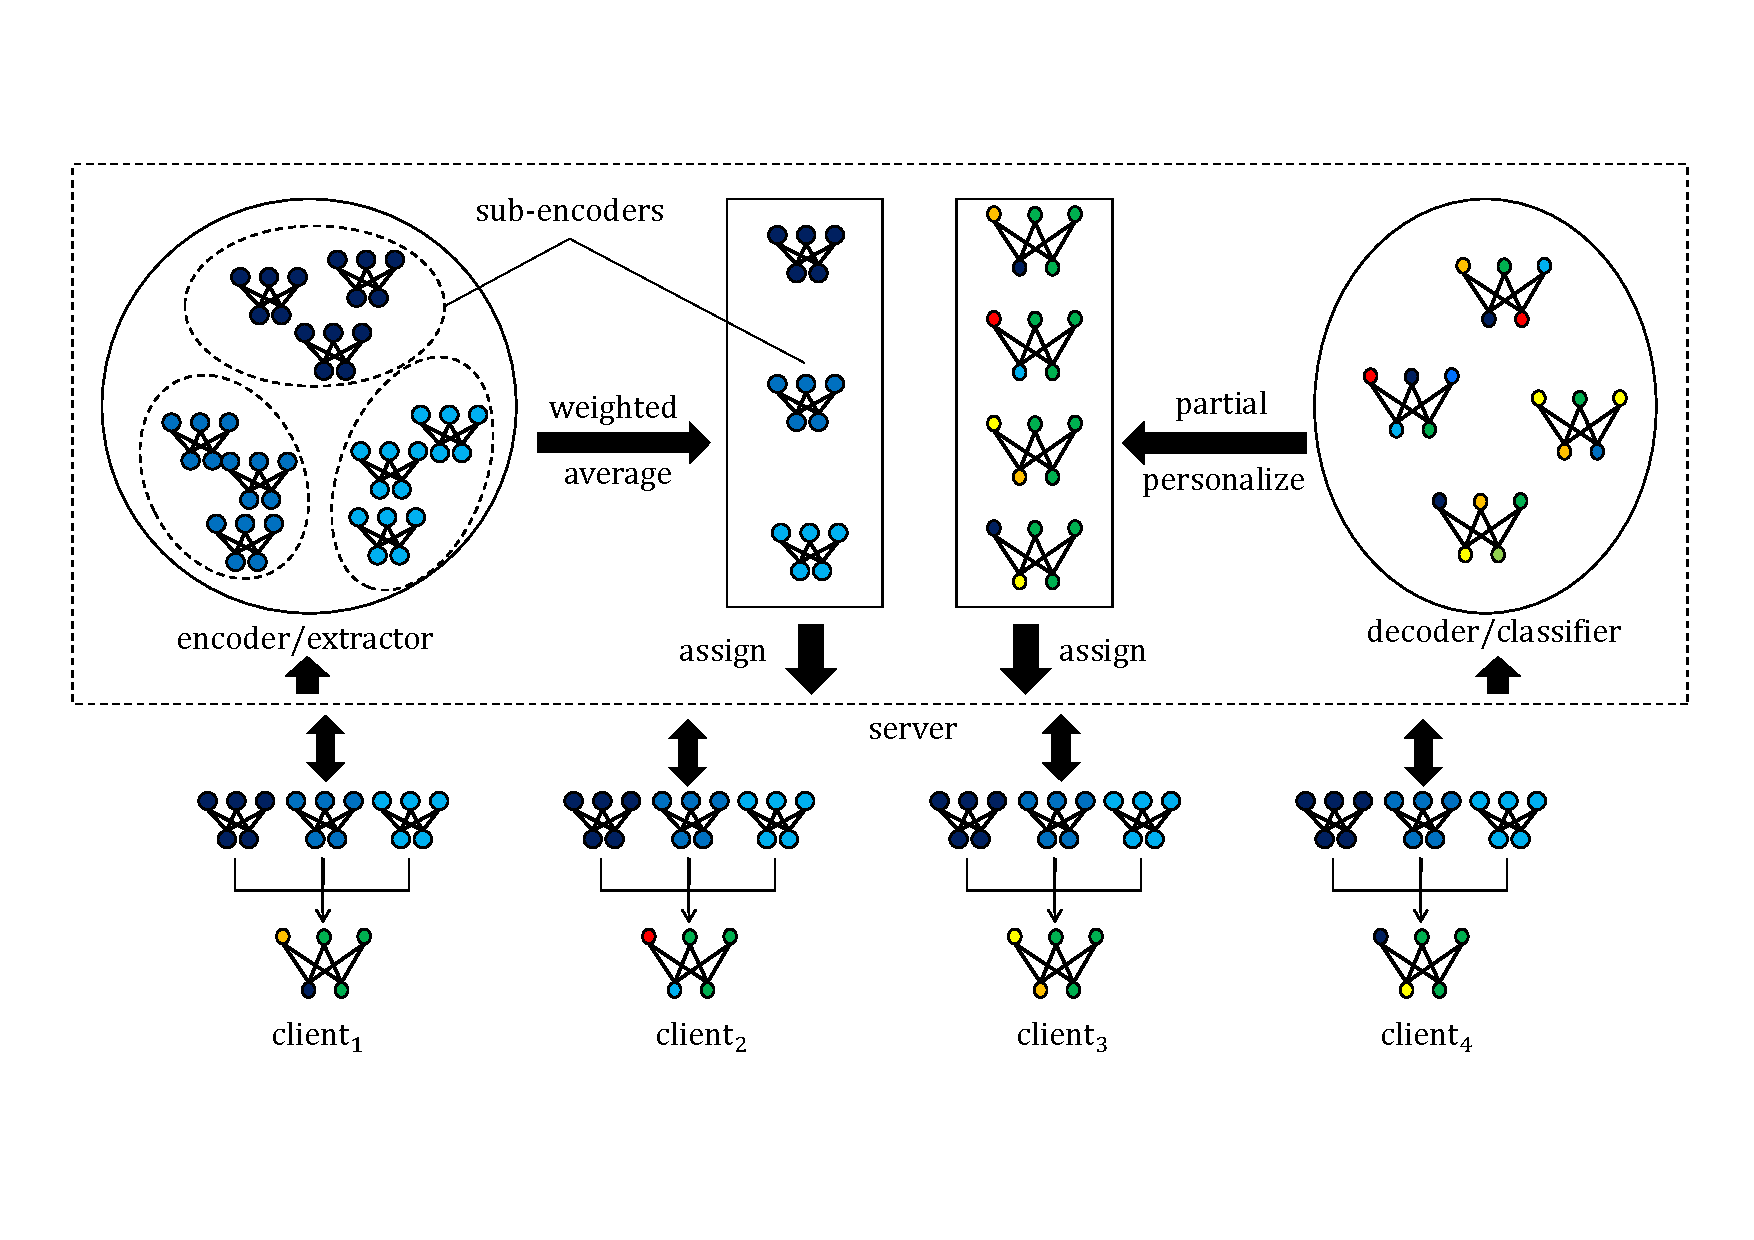
\includegraphics[scale=0.25,trim=0 100 0 0]{./picture/whole_model.pdf}}
	\subfigure[structure of network]{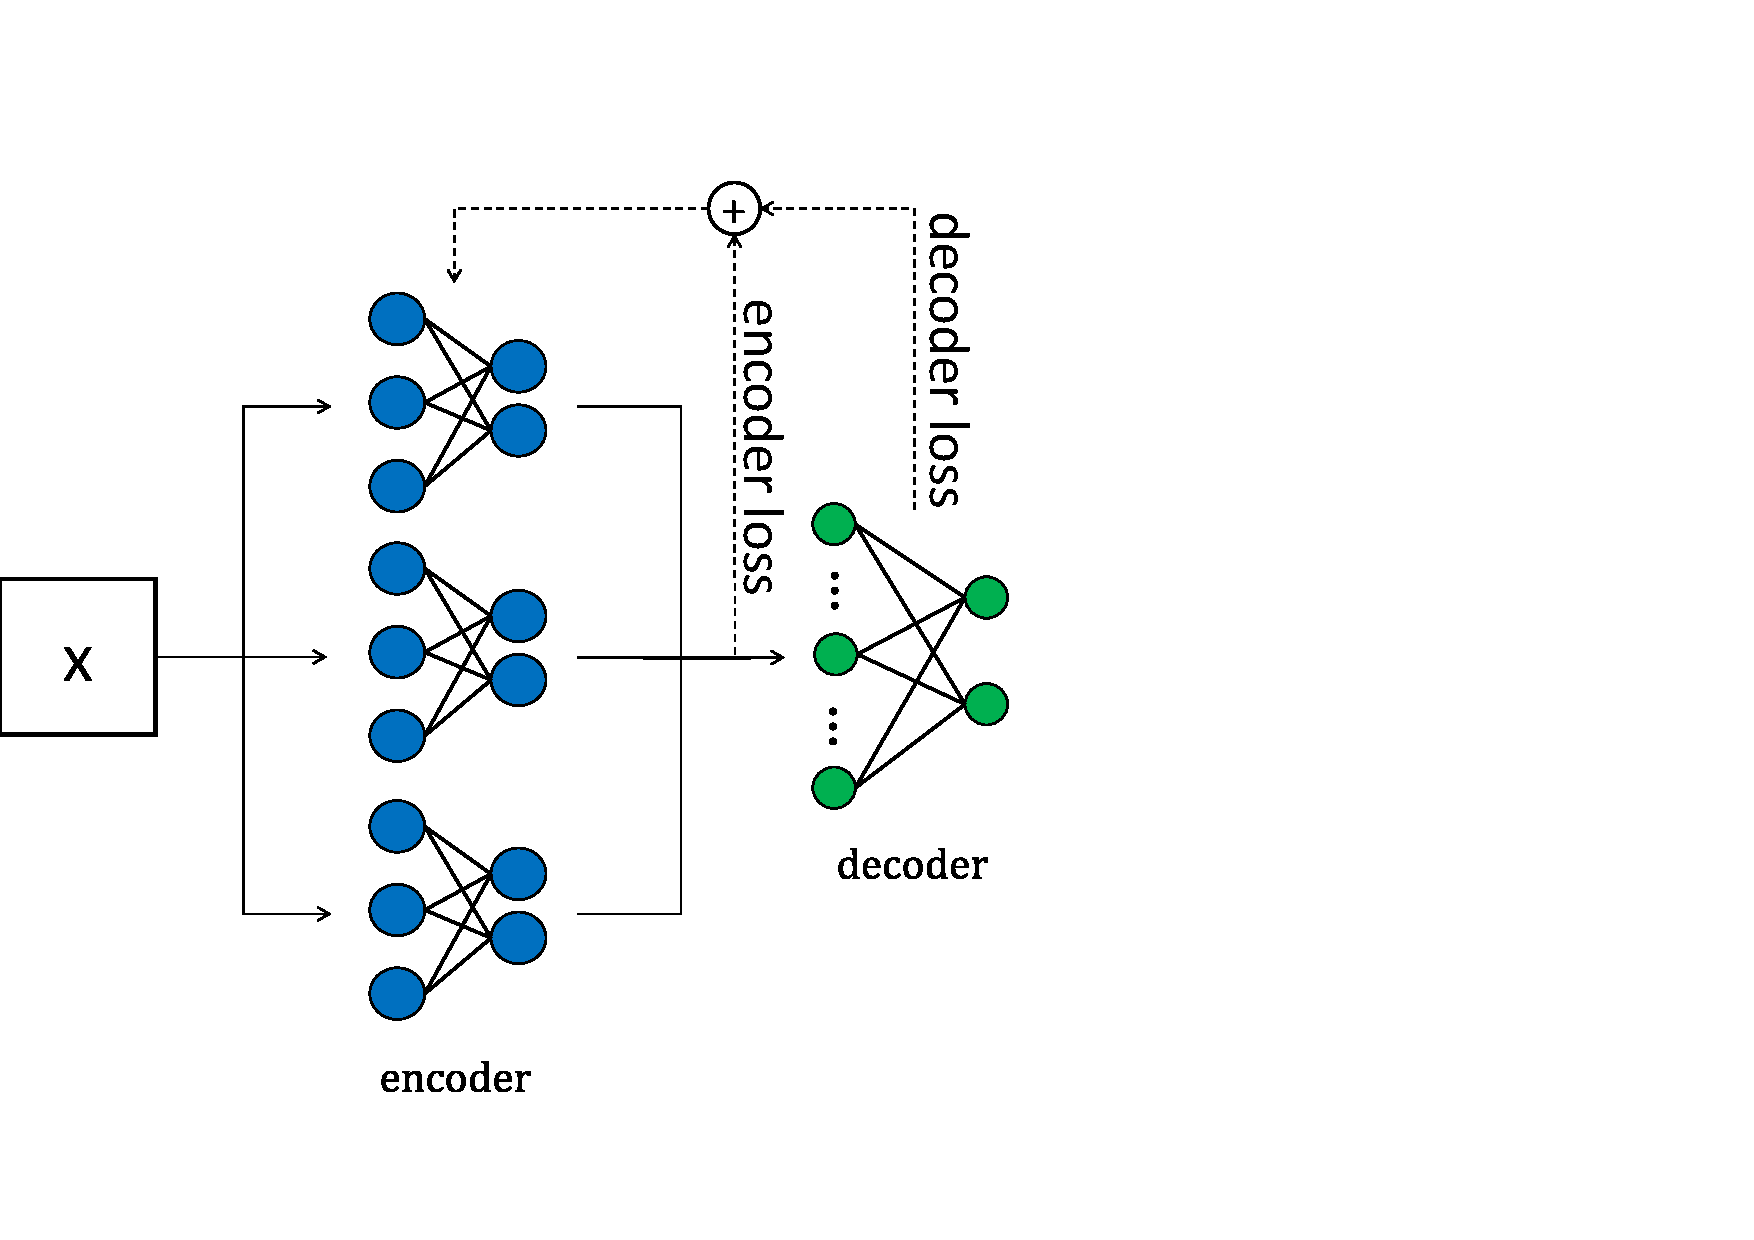
\includegraphics[scale=0.16,trim=0 100 300 100]{./picture/model1.pdf}}
	\subfigure[decoders' components]{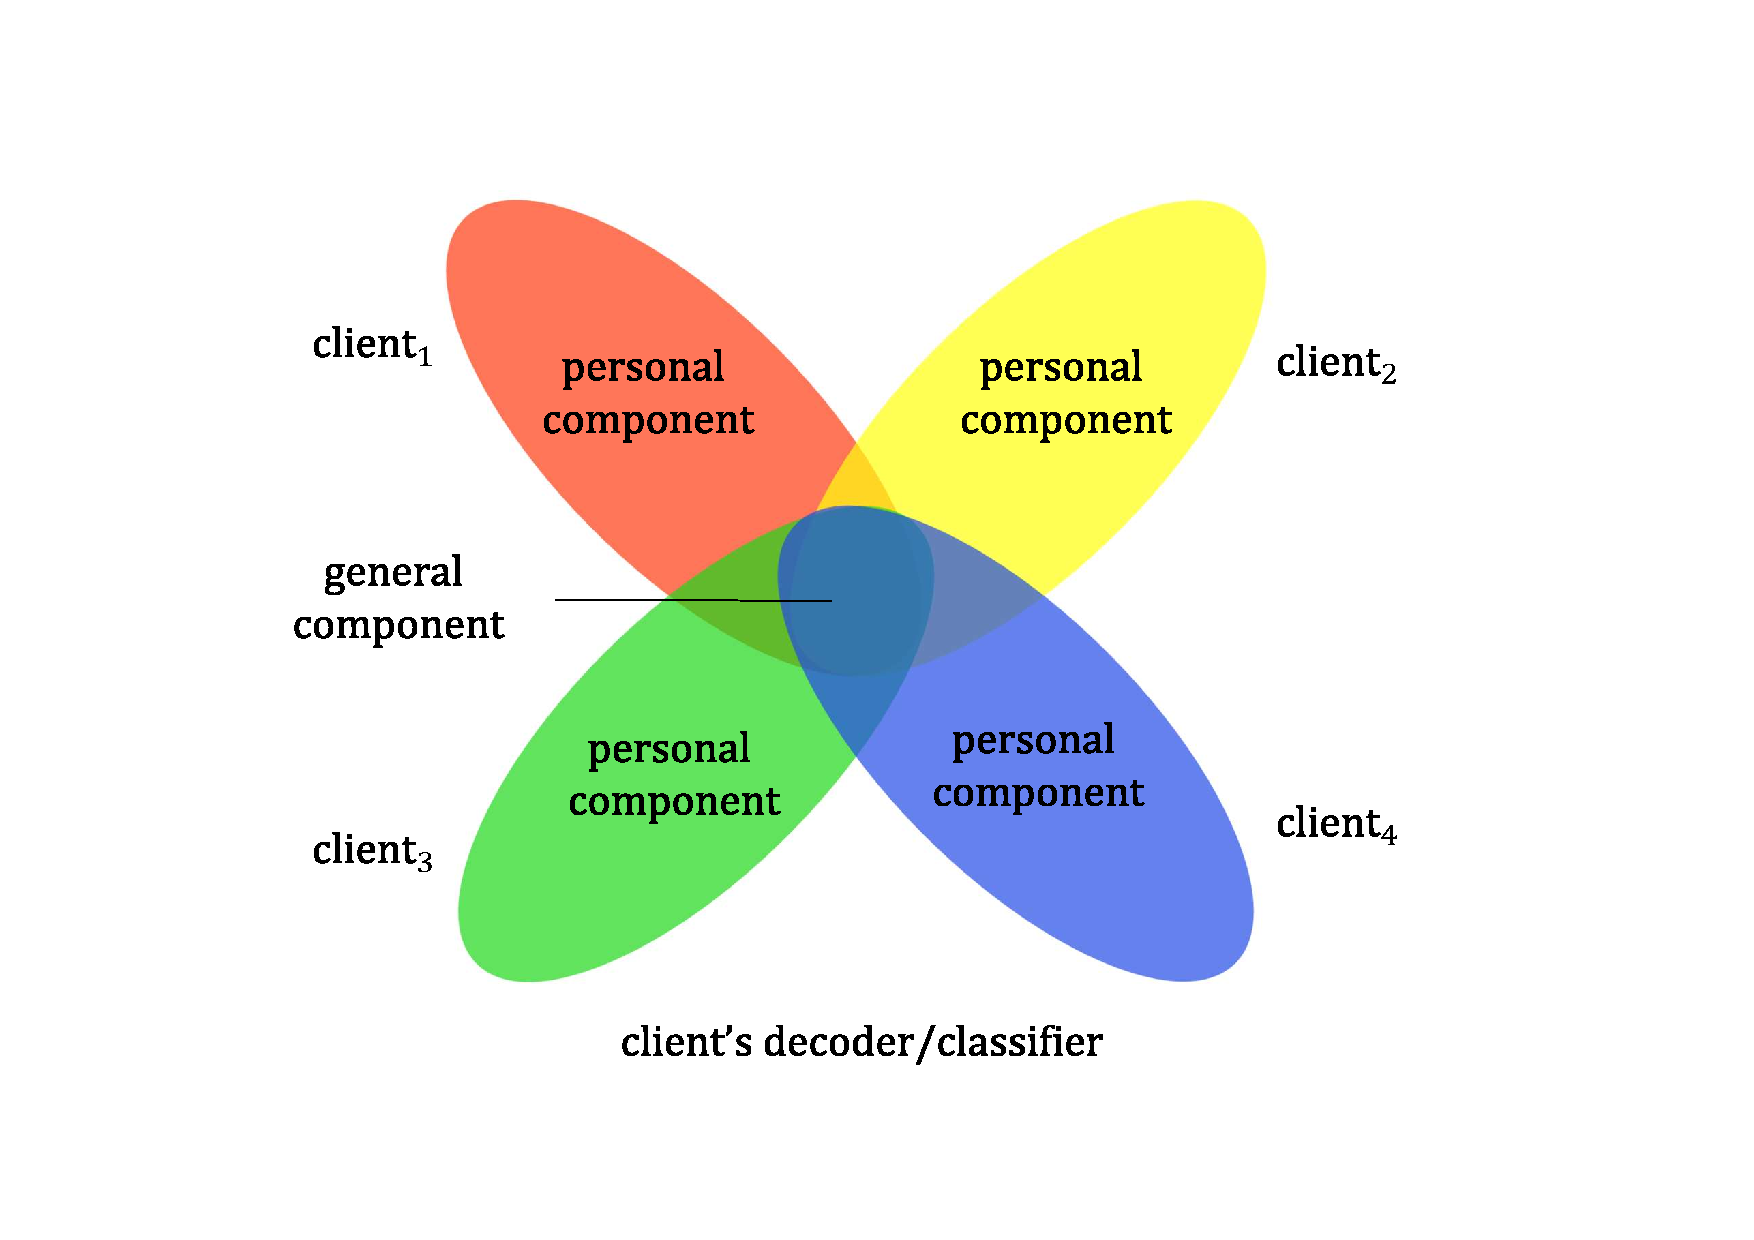
\includegraphics[scale=0.16,trim=0 100 100 100]{./picture/classifier_part.pdf}}
	\caption{Each client shares one network structure which is consist of several sub-encoders and one decoder. The server aggregates sub-encoders' and partial decoders' parameters which are considered as general component from clients through weighted averaging. Personal component which are great different among client in decoders are maintained its' parameters doing not take part in aggregation. Sub-encoders align features through encoder loss prompting models' specificity. Decoder keep its' personal parameters to ensure models' accuracy in different distribution data.}
	\label{fig_model}
\end{figure}

Our contributions are as follow:
\begin{itemize}
	\item We propose sub-encoder which major in extracting one category data feature. This structure aligns identical category features in different clients.
	\item We design an aggregating strategy suiting for sub-encoders' parameters. Each sub-encoder is assigned maximum weight in its' major field.
	\item Different from other personalized strategy which applied regularization to aggregate, FedDiv reserves part raw weight through divergence among clients. This way is efficiently and effectively that suits large-scale federated learning.
	\item We improve models' performance in sensitiveness and specificity by aligning sub-encoders and prompt their accuracy by personalizing decoder. 
\end{itemize}

\section{Related work}

\subsection{personalized federated learning}
Traditionally, the global model is updated by using distributed private data in federated learning, and lots of optimization methods have been proposed.  FedAvg\cite{McMahan2016CommunicationEfficientLO} and FedProx\cite{Sahu2018FederatedOI} are representative strategies in generic federated learning. With the advanced study on federated learning, researchers encounter severe problem of non-IID data \cite{xxx}. Nowadays,  personalized federated learning has drawn much attention due to its' higher accuracy \cite{Zhu2021FederatedLO}. There are many personalized methods to aggregate models including regularization \cite{xx}, clustering \cite{xx}, feature aligning \cite{xx} and so on. Specifically, the regularization strategy's basic idea is to guide the local model aggregating direction by global information. Among them, FedAMP\cite{Huang2020PersonalizedCF} and L2GD\cite{Hanzely2020FederatedLO} learn personalized models {\textbf{being lead by each other local models}}. Similar to FedAMP, FPFC\cite{Yu2022ClusteredFL} combines clustering and regularization. In many strategies, the cost of computational resources will increase high with the participants mounting up, when introducing regularization to federated learning. That may limit these methods applied into federated learning. However, strategies based on clustering methods like IFCA \cite{Ghosh2020AnEF} and FedBayes \cite{Zhang2022PersonalizedFL} would raise the communication cost. We think that the process of federated learning is dynamic and the extent of personalizing is decided by the guiding ability of global information. Thus, we assume that adjusting the models' extent of personalizing through divergence would reach similar effect at a low cost way.

Comparing with those existing methods, the proposed method gains following advantages. First, xxx. Second, xxxx.



\subsection{personalized federated learning based on feature aligning}
It is not enough that purely personalized aggregate models and most people merge model calibration into model personalization. Someone had chosen realistic or virtually balanced data to align models \cite{Luo2021NoFO,Shang2022FEDICFL,Zhao2018FederatedLW}. However, this data may not obey actual distribute or even violate the principle of federated learning. Others had used divergence calibrate the models but they didn't consider whole category consistency \cite{Li2022RobustAF,Zhang2021FederatedLF}. Normalization in data is one way to align features being extracted by encoders but it still could not avoid distribution of data in various clients affect to model training \cite{Li2021FedBNFL}.  FedRoD\cite{Chen2022OnBG} suggested that the features can be aligned by balanced softmax loss and this strategy had performed excellently in metric of accuracy. But it ignores the minority while pay attention to majority which would make it in disadvantage when we compare sensitiveness and specificity. To ease this problem meanwhile calibrate models, we design sub-encoders which pay attention to one class data.  The superiority includes xxxx.

Contrastive learning is another way to calibrate models. Among unsupervised or semi-supervised learning, it plays an important role. Weiming Zhuang et al.  choose siamese network to execute that task \cite{Zhuang2022DivergenceawareFS}. And this network aims to find out the difference between different category meanwhile search for identical features among same group. However, without the guidance of label, the learning efficiency will be low and the model will perform below expectations. Felix X. Yu et al\cite{Yu2020FederatedLW} propose similar ideas to train networks with only positive labels though they used distance instead of divergence to align features. FedIIC\cite{Wu2022FedIICTR} considered the difference and similarities among classes, but it took so much hyper-parameters that the complexity was increased. Although FedABC\cite{Wang2023FedABCTF} transformed multi-classify task to double-classify task, disproportion between positive and negative samples would hinder classifiers discriminate them. Different from these strategies, we calibrate extractors or encodes by limiting divergence for each category features to extract more generic features.  



\section{Preliminaries}
In this section, we briefly introduce the generalizing or personalizing methods of federated learning. Generally, generic models are easily be transplanted to new clients but it's accuracy are normally lower than personal models. Personalizing federated learning usually get higher quality models but there are some problems like sensitiveness and specificity maintained to be solved \cite{Kulkarni2020SurveyOP}.

\subsection{Federated learning}
The global loss function learned from several clients is defined as

\begin{align}\nonumber
	\min\limits_{W} L(W):=\sum_{k=1}^{K}\frac{L_{k}(W)}{K}.
\end{align}
Here, $W$ denotes model's parameters; $K$ represents the total number of clients. As the representative aggregation strategy,  FedAvg iteratively update model between server and clients \cite{McMahan2016CommunicationEfficientLO}. At server, it performs
\begin{align}
\nonumber
W=\sum_{k=1}^{K}\frac{n_{k}}{n}W^{k},
\end{align} where $W^{k}$ is obtained by performing 
\begin{align}
\nonumber
W^{k} = \argmin_{U} L^{k}(U).
\end{align}
Intuitively, federated learning aggregates every clients' knowledge by using distributed data. But it will be mislead by unbalance of data. Especially when some clients' data is non-IID,  the generic federated learning strategy will be impeded \cite{Li2021FederatedLO}.

\subsection{Personalized federated learning}



\subsection{Tradeoff between personalized and generic federate learning}
Someone argues that the data distribution varies in clients for their different attribute. Learning a global model may ignore clients' unique characteristic. Personalized federated learning suggests that we should train local model for each client from a global model. There are many methods to deal with it such as regularization, fine tuning and so on. These methods produce many excellent results. There are some shortages waiting for being overcomed in applications such as multi-center medical analysis.
\begin{itemize}
	\item Some methods are trying to trade off non-IID data against IID data. When it executes well in non-IID data, it may perform poorly during dealing with IID data. While the medical industry cases includes both non-IID data and IID data.
	\item Many strategies pay attention to accuracy while overlook others metrics such as sensitiveness and specificity. Hospitals need different indexes in different scenes for example it requires high sensitiveness for screening experiment while making a definite diagnosis must be high specificity.
	\item Lots of algorithms could not solve the problem that disadvantage cases are covered by advantage cases. If the number of one category instances far more than another, the advantage category data are possibly covering whole networks causing the disadvantage category data learning insufficiently.
\end{itemize}

To overcome the problems mentioned above, we propose FedDiv. The strategy aggregates encoder and decoder in different way. We divide encoder into many small parts and aggregate decoder according to the data divergence.

\section{FedDiv}
In deep learning, the network usually is consist of encoder/extractor and decoder/classifier. And in this section we call it encoder and decoder. While, single encoder may be mislead by unbalanced data easier than multi-encoder. We can train personal encoder for each local data but it is unnecessary. Because each category data should has identical feature. And it should not be noised by distribution of data when the encoder extracts features. Because of depending on the possibility output by encoder, the decoder should be changed to adapt various data with different distribute.

\subsection{Multiple Encoder}
We hold the idea that encoder should abstract same features from identical category data, but single encoder will be mislead by non-IID data. We designed a loss function for encoders each of that focus on one category data. We assumed that if there are category-special feature, the more convergent the feature is, the more general it will be. And the loss function can be formula as follow:
\begin{align}\label{encoder_std}
	%\min\limits_{\theta} L_{e}(\theta;x)=\sum_{i=1}^{C}D(encoder_{i}(\theta^{i};x))
	L_{e}(\boldsymbol{\theta}_{1},...,\boldsymbol{\theta}_{C};\boldsymbol{x})=\sum_{i=1}^{C}D(\beta_{i}(\boldsymbol{l})\phi_{i}(\boldsymbol{\theta}_{i};\boldsymbol{x})) .
\end{align}
Here, $D(\cdot )$ represents divergence and we we choose \textbf{standard deviation} (STD) to measure the features' divergence output by encoder in this article. $\phi_{i}(\cdot)$ is $i$th encoder or extractor in the net. It outputs features with the form as:
\begin{align}\nonumber
	\phi_{i}(\boldsymbol{\theta}_{i};\boldsymbol{x})=F.
\end{align}
$\boldsymbol{\theta}_{i}$ is the parameter of $i$th encoder $\phi_{i}$. $C$ is the number of category. And $F \in R^{B\times N}$ represent features which are extracted by $\phi_{i}$ from inputs $\boldsymbol{x}\in R^{B\times 1}$. $\beta_{i}(\boldsymbol{l})$ is focus coefficient lead by label $\boldsymbol{l}\in R^{B\times 1}$. $B$ is the number of encoders. $N$ is the number of features output by one encoder from $i$th input $\boldsymbol{x_{i}}$. Finally, the $D(\cdot)$ is formulated as:
\begin{align}\label{classification_eloss}
	D(\beta_{i}(\boldsymbol{l})\phi_{i}(\boldsymbol{\theta}_{i};\boldsymbol{x}))=\sum_{j=1}^{N}\frac{std(\beta_{i}(\boldsymbol{l})\odot F_{:,j})}{N}.
\end{align}
Here, $F_{:,j}$ represents $j$th feature which is extracted by encoders. $N$ represents that the input can be extracted to $N$ features. We called Equation \ref{encoder_std} as divergence loss.

There are some different between classification task and segmentation task. Because in classification task the encoder extracts features belong to one category data only. While all category features exist in identical outputs when encoders take segmentation task.

\subsubsection{Classification task}
In classification task, each category input can be extracted as $N$ unique features. If their divergences are small, we consider that the feature's variation should be small in new data. So, we hold some opinion:
\begin{itemize}
	\item Identical category data share same features.
	\item If features extracted by encoder from identical category data in training datasets are highly concentrating, it is quite possible that these features also exist in test training datasets and their variation is small.
\end{itemize}

According to above mentioned, the focus coefficient $\beta_{i}(\boldsymbol{l})$ is formulated as:
\begin{align}\label{classification_belta}
	\beta_{i}(\boldsymbol{l})=e^{\lambda(2\delta(\boldsymbol{l}-i)-1)}.
\end{align}
Here, $\delta(\cdot)$ is unit pulse sequence. $\beta_{i}\in R^{B\times1}$ is focus coefficient. Figure \ref{fig_classification_encoder_backward} shows this procession.


\begin{figure}
	\centering
	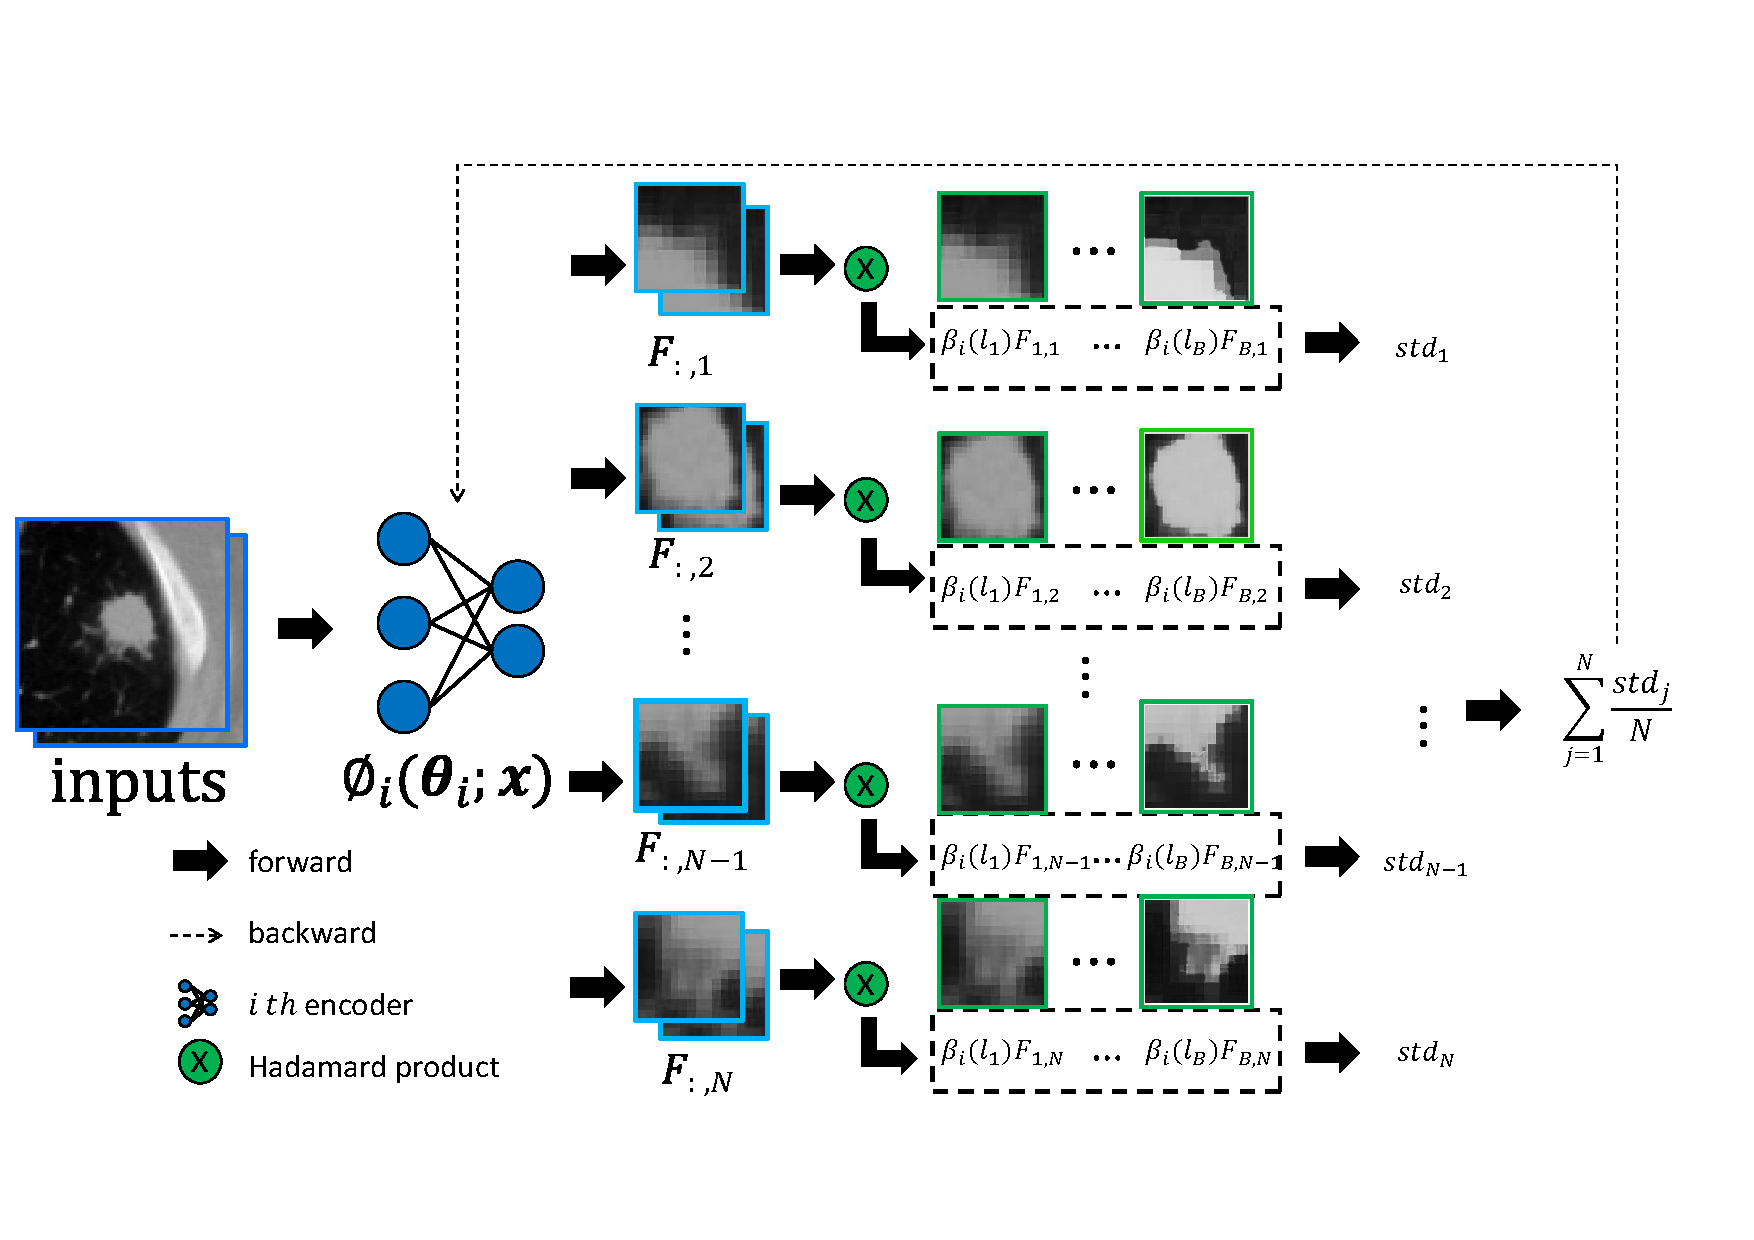
\includegraphics[scale=0.25]{./picture/encoder_loss_backward.pdf}
	\caption{\textbf{Divergence loss in classification task}. Each category data can be extracted as $n$ unique features. Focus coefficient $\beta_{i}(\boldsymbol{l})$ in Equation \ref{classification_belta} varies to different category data.}
	\label{fig_classification_encoder_backward}
\end{figure}

\subsubsection{Segmentation task}
Segmentation task is different from classification task, because all the category features exist in identical outputs. There are several assumption in the segmentation task:
\begin{itemize}
	\item Most time, targets' edge are blurry and dimmed. We need enhance the edge's features.
	\item The features from background are small than from target in medical data. To balance this difference, features from background should have larger coefficient.
	\item The target's relative position is unchanging in encoder's output with encoder becoming deeper. And the encoders' outputs are tensor with different scale.
\end{itemize}

From above assumption, we think that the extent of divergence should be negative correlation with the distance of the target's center and we use average pooling to replace it. So we design $\beta_{i}(\boldsymbol{l})$ as:
\begin{align}\nonumber
	\beta_{i}(\boldsymbol{l})=\lambda e^{-p_{i,:}(\boldsymbol{l}^{\gamma })} .
\end{align}
Here, $p_{i,j}(\cdot)$ represents average pooling which output consequence with same size as $F_{i,j}$. Labels $\boldsymbol{l}_{i}$ are tensors and feature $F_{i,j}\in R^{d_{j,1}\times d_{j,2}} $ means $j$ th feature from $i$th input. The feature's size is related with the depth of encoder. $p_{i,j}(\boldsymbol{l}^{\gamma}) \in R^{d_{j,1}\times d_{j,2}}$ means $i$th input label that is averaged pooling matching with identical size of  $F_{i,j}$. $\gamma$ is hyper-parameters which determines the average pooling edge sharpness of $i$th input. $\lambda$ controls the average pooling strength of input. We can refer the Figure \ref{fig:segmentation_encoder_backward}.
\begin{figure}
	\centering
	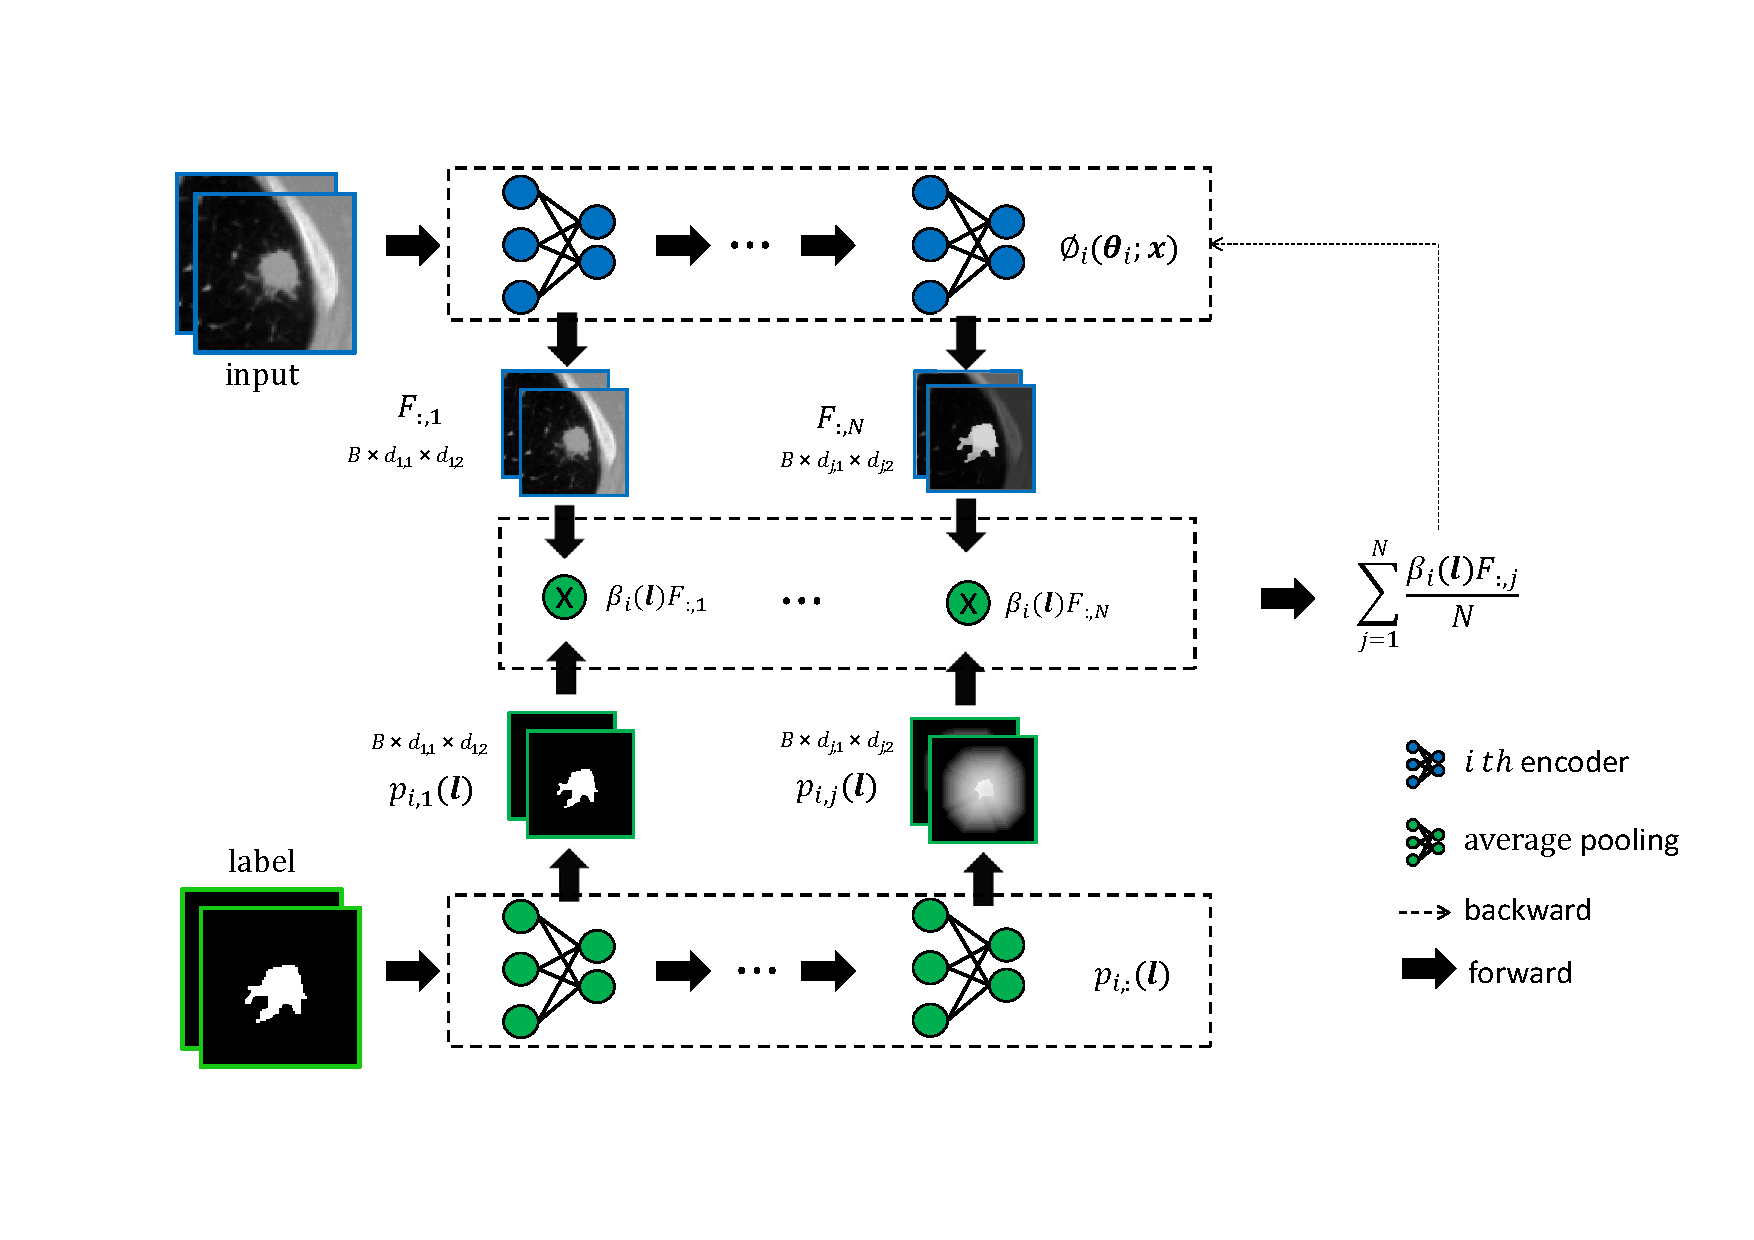
\includegraphics[scale=0.25]{./picture/seg_encoder_back.pdf}
	\caption{\textbf{Divergence loss in segmentation task}. The target's relative position is unchanging in encoder's output though size of output is unequal to that of input. The extent of divergence should be negative correlation with the distance of the target's center.}
	\label{fig:segmentation_encoder_backward}
\end{figure}


We connect the encoders with a decoder and make a decision. On the whole, this network is composed of several encoders and one decoder. Its loss function is formula as two parts:
\begin{align}\label{whole_loss}
	\min\limits_{\Theta} L(\Theta)=L^{\star}(\Theta;X)+\alpha L_{e}(\Theta;X) .
\end{align}
Here, $K$ is the number of client. $L^{\star}$ is risk loss function. $L_{e}$ is the divergence loss. Normally, we choose entropy-cross loss function as $L^{\star}$ that is mainly extracting the dividable features. But the features caught by entropy-cross loss function may not be general because it focuses on features' divisibility in training data. So, we add divergence loss to re-catch the encoder's attention on the generalization of features.

\subsection{Personal Decoder}
Thinking about the scene that the divergences of some encoders' output are tiny in same class data while decoders' parameters which correspond with the outputs vary widely in different client, we guess that these features encoded by encoders is client-only. Generally speaking, if the symptom in chinese pneumonia patients is cough while that in America more likely is dyspnea, we should aware that this symptom maybe regional or ethnically diverse. The symptom represents the output of encoders and different symptom make different decision meaning that decoders' parameters vary among countries. In discussion, they will have reservation if they disagree others' opinions. Thus, referring to similar scene, we personalized decoder according to its divergence. This procession can be indicated by Algorithm \ref{personalize_algorithm}. And we can transform the mentions above to equation:

\begin{align}\label{divergence_aggregate}
	\varphi^{k}_{t}=\varphi^{k,*}_{t}-(\varphi^{k,*}_{t}-\bar{\varphi}^{k}_{t})g(std(\Phi^{k}_{t})) 
\end{align}
 Here, $\varphi^{k}_{t}$ is the parameters which should be sent to $k$th client after aggregating in $t$th iterations. $\varphi^{k,*}_{t}$ is the decoder's parameters returned by $k$th client in $t$th iterations. $\bar{\varphi}^{k}_{t}$ is  mean value of $n$ clients nearing $k$th client. $\Phi^{k}_{t}$ is a matrix being consisted of parameters from $n$ clients nearing $k$th client. $g(\cdot)$ is the selection function according to the divergence of clients' parameters. In this paper, we formulate the selection function as:
\begin{align}\label{personal_select}
	g(x)=e^{-(\lambda x)^{\gamma}} 
\end{align}
If $\gamma>1$, the function includes three part:
\begin{itemize}
	\item $g=1$, means that local parameters are mean value when the divergence is small.
	\item $g\approx kx+b$, means that local parameters are linearly leaded by mean value.
	\item $g=0$, means that local parameters are personalized value when the divergence is big.
\end{itemize}

We set $\gamma=10$ that will transform it to be hard selection function. When $\lambda x>1$, we think  $x$ is personal parameter while $x$ is global parameter if $\lambda x<1$. And we should notice that parameters' divergence will be larger with aggregation turns increasing. It can be regard as there are more local parameters in the end of aggregation. We consider that this phenomenon is benefit to aggregation because in the beginning of aggregation the models are insufficient training and they need more global parameters to guide the local learning. Figure \ref{fig_personalize_aggregation} shows the procession of aggregation.

\begin{figure}
	\centering
	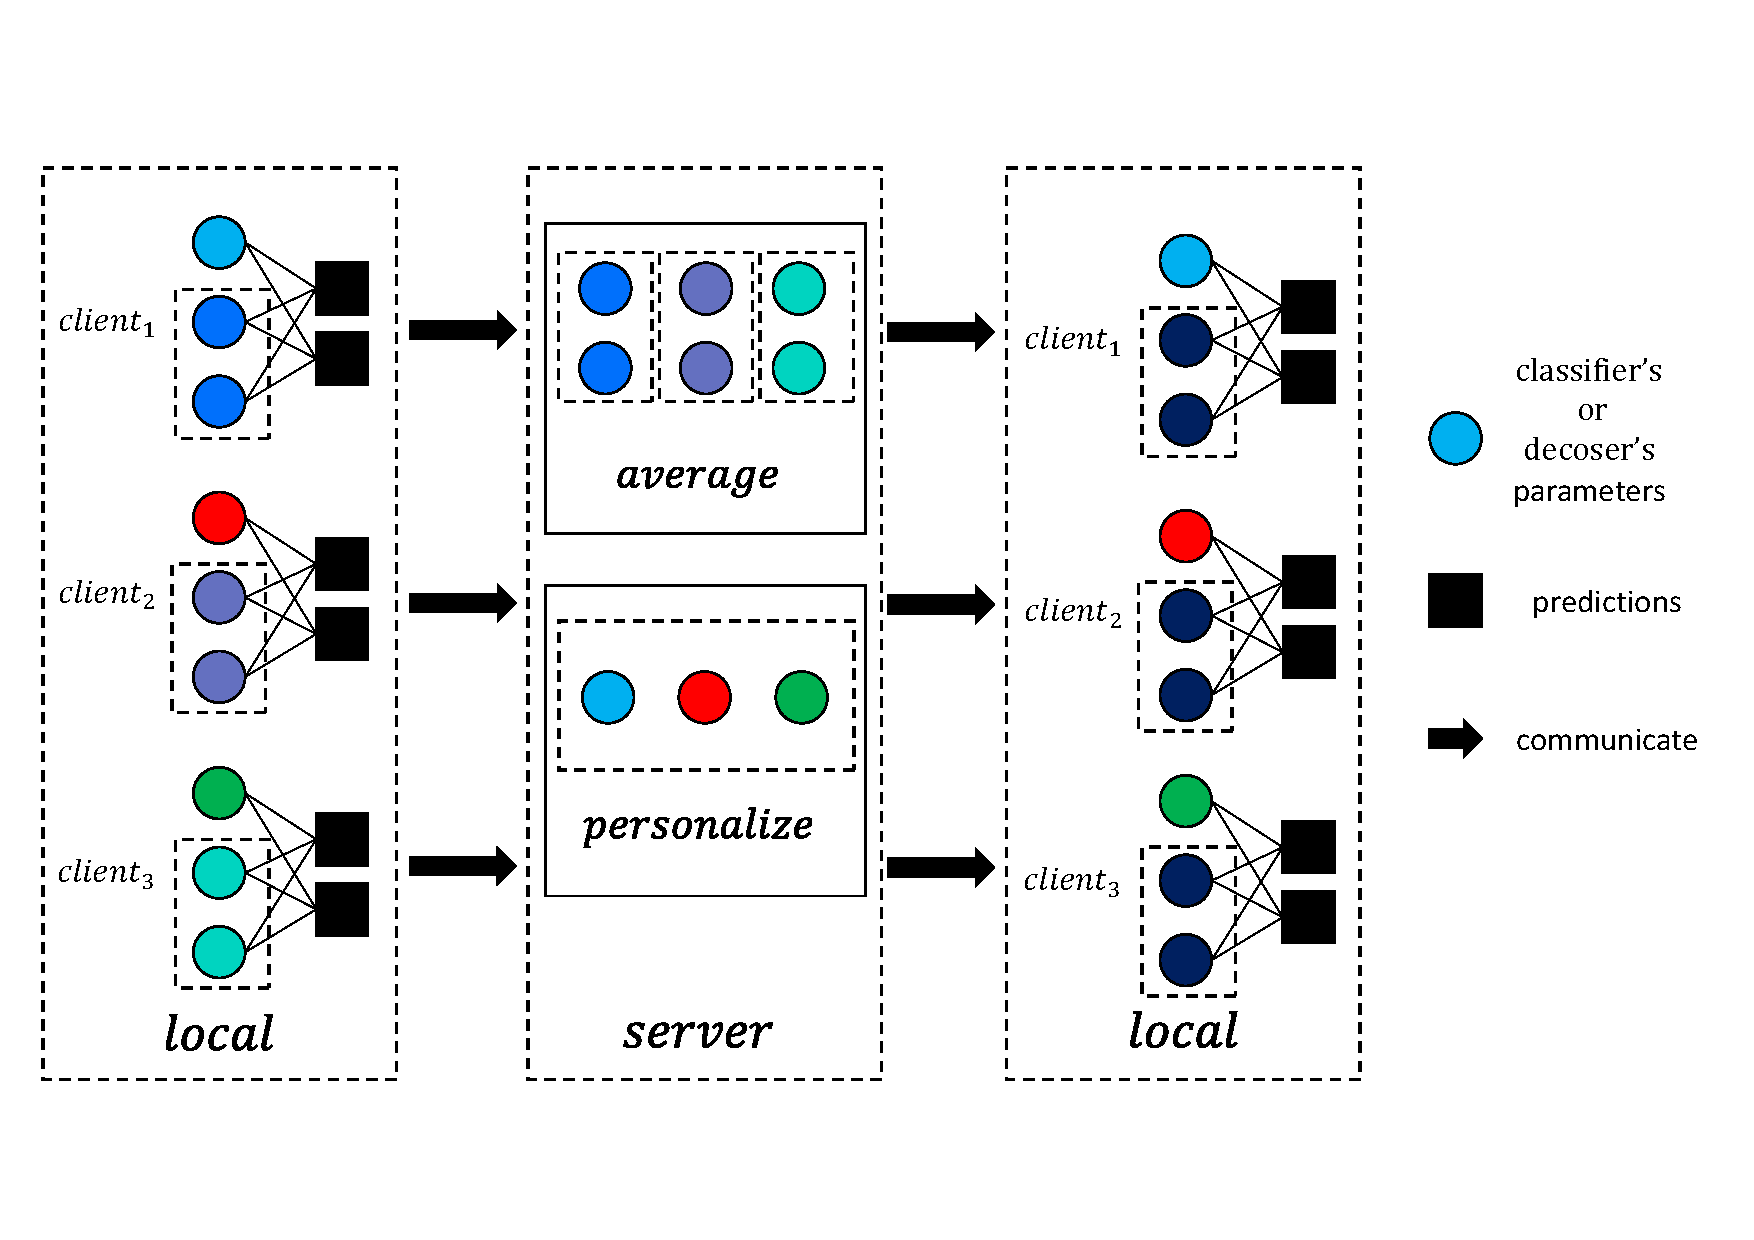
\includegraphics[scale=0.25]{./picture/personalize_aggregation.pdf}
	\caption{\textbf{Aggregation of classifier's or decoder's parameters}. Parameters will be aggregated in average when the local parameters' divergence is small. If their divergence is large, the local parameters will be reserved and dose not take part in aggregating. What the parameter should be, is decided by Equation \ref{personal_select}.}
	\label{fig_personalize_aggregation}
\end{figure}

\begin{algorithm}
	\caption{personalized aggregation}\label{personalize_algorithm}
	\textbf{Server : ($t=1,2,...,T $)} 
	\begin{algorithmic}[1]
		\While{$t<T+1$}
		\State get decoders' parameters $\varphi^{k,*}_{t}$ from clients
		\State  aggregate $\varphi^{k,*}_{t}$ by eq \ref{divergence_aggregate} and outcome $\varphi^{k}_{t}$
		\State Send  $\varphi^{k}_{t}$ to client.
		\EndWhile
	\end{algorithmic}
	\textbf{Client $k$ : ($t=1,2,...,T $)} 
	\begin{algorithmic}[1]
	\While{$t<T+1$}
	\State get decoder's parameters $\varphi^{k}_{t}$ from server
	\State $\theta^{i,k,*}_{t} \gets \min\limits_{\theta} [f(\bar{\theta}^{i}_{t-1},\varphi^{k}_{t};x)+\alpha L_{e}(\bar{\theta}^{i}_{t-1},\varphi^{k}_{t};x)] $
	\State Send encoder's parameters $\theta^{i,k,*}_{t}$ to server.
	\EndWhile
\end{algorithmic}

\end{algorithm}


\subsection{Algorithm}
We argue that identical data shares same feature in different clients. Thus, the encoders' parameters in each client should be same. We aggregate each class-special encoder through class weighted average in Algorithm \ref{gloabal_algorithm}. And we formulate the aggregation function:

\begin{align}\label{encoder_aggregate}
	\bar{\theta}^{i}_{t}=\sum_{k=1}^{K}\frac{N^{i}_{k}\theta^{i,k,*}_{t}}{N^{i}}
\end{align}
The Equation \ref{encoder_aggregate} outcomes same parameters in identical category-favor encoders which handle certain kind of category data in preference to others. Where, $\bar{\theta}^{i}_{t}$ is aggregation weight in class-favor encoder. $N^{i}_{k}$ is the number of $i$th class in $k$th client while $N^{i}=\sum_{k=1}^{K}N^{i}_{k}$ is total number of $i$th class data. $\theta^{i,k,*}_{t}$ is $k$th client returned $i$th class-favor encoder's parameters. 

\begin{algorithm}
	\caption{Class weighted aggregation}\label{gloabal_algorithm}
	
	\textbf{Server : ($t=1,2,...,T $)} 
	\begin{algorithmic}[1]
		\While{$t<T+1$}
		\State get encoders' parameters $\theta^{i,k,*}_{t}$ from clients
		\State aggregate $\theta^{i,k,*}_{t}$ by eq \ref{encoder_aggregate} and outcome $\bar{\theta}^{i}_{t}$
		\State Send  $\bar{\theta}^{i}_{t}$ to client.
		\EndWhile
	\end{algorithmic}
	
	\textbf{Client $k$ : ($t=1,2,...,T $)}
	
	\begin{algorithmic}[1]
		\While{$t<T+1$}
		\State get encoder's parameters $\bar{\theta}^{i}_{t}$ from server
		\State $\varphi^{k,*}_{t} \gets \min\limits_{\varphi}f(\bar{\theta}^{i}_{t},\varphi^{k}_{t-1};x) $
		\State Send decoder's parameters $\varphi^{k,*}_{t}$ to server.
		\EndWhile
	\end{algorithmic}
\end{algorithm}

\begin{algorithm}
	\caption{FedDiv}\label{FedDiv_algorithm}
	
	\begin{algorithmic}[1]
		 
		\item \textbf{Server :}
		\item \enspace\textbf{Initialize:} send $\bar{\theta}^{i}_{0},\varphi^{k}_{0} $ to clients
		
		\item \enspace Aggregate $\boldsymbol{\theta}$ according Algorithm \ref{gloabal_algorithm}
		
		\item\enspace Aggregate $\boldsymbol{\varphi}$ according Algorithm \ref{personalize_algorithm}
		
		\item\textbf{Client :} 
		
		\item\enspace Update $\boldsymbol{\theta}$ and send $\boldsymbol{\varphi}$ according Algorithm \ref{gloabal_algorithm}
		
		\item\enspace Update $\boldsymbol{\varphi}$ and send $\boldsymbol{\theta}$ according Algorithm \ref{personalize_algorithm}

	\end{algorithmic}
	
\end{algorithm}
Here, $\boldsymbol{\theta}$ and $\boldsymbol{\varphi}$ represents sub-encoders' parameters and decoder's parameters respectively. It describes the whole process of FedDiv. We use the method of alternatively optimizing between encoder and decoder. It transmits whole parameters in each two communications, therefor the strategy doesn't increase the cost of communication. In a word, we firstly find general feature through class-favor encoders and get personal model through personalized decoder.

\section{Experiments}
In this section, we will display the performance of FedDiv and compare it with others strategies including two generic federated leaning algorithms and twelve personalized federated learning algorithms. We chose FedAvg\cite{McMahan2016CommunicationEfficientLO} and FedProx\cite{Sahu2018FederatedOI} as comparable algorithm. While the personalized algorithms include FedAMP\cite{Huang2020PersonalizedCF}, FedRoD\cite{Chen2022OnBG}, L2GD\cite{Hanzely2020FederatedLO} and so on.

\subsection{Setting and material}

\subsubsection{\textbf{Metric}}
In classification task, we used \textbf{best mean accuracy} (BMACC)\cite{Huang2020PersonalizedCF} to evaluate total performance of strategy and \textbf{best mean balance accuracy} (BMBACC), \textbf{best mean class-average F1 score} (BMCAF1) and \textbf{best mean specificity} (BMSpec) to estimate their performance in each class. BMACC is the highest averaging accuracy of all clients in whole communicating period. BMBACC is the official metric of the ISIC 2019 Challenge \cite{Wu2022FederatedLW}. They can be formula as:
\begin{multline}\label{BMBACC_func}
	BMBACC= 
	\frac{1}{N_{client}N_{class}} \sum_{k=1}^{N_{client}}\sum_{i=1}^{N_{class}}\frac{TP_{i,k}}{TP_{i,k}+FN_{i,k}}.
\end{multline}
\begin{multline}\nonumber
	BMACC= \frac{1}{N_{client}} \sum_{k=1}^{N_{client}}\frac{\sum_{i=1}^{N_{class}}TP_{i,k}}{N_{k}}.
\end{multline}
In fact, BMBACC is mean sensitive in each category data and we adhere the reference \cite{Wu2022FederatedLW} calling it BMBACC. 
Corresponding to it, \textbf{best mean specificity} (BMSpec) can be formulated as:
\begin{multline}\nonumber
	BMSpec= 
	\frac{1}{N_{client}N_{class}} \sum_{k=1}^{N_{client}}\sum_{i=1}^{N_{class}}\frac{TN_{i,k}}{FP_{i,k}+TN_{i,k}}.
\end{multline}
To more effective estimate the strategy's ability of distinguish different category data, we refer to BMBACC and defined F1 score in different category as BMCAF1 which can be formula as follow:
\begin{multline}\nonumber
	BMCAF1= \\
	\frac{1}{N_{client}N_{class}} \sum_{k=1}^{N_{client}}\sum_{i=1}^{N_{class}}\frac{2TP_{i,k}}{FP_{i,k}+FN_{i,k}+2TP_{i,k}}.
\end{multline}
Here, $N_{client}$ is the number of clients. $N_{class}$ is the number of class. $TP_{i,k}, TN_{i,k}, FP_{i,k}$ and $FN_{i,k}$ represent true positive, true negative, false positive and false negative of class $i$ in $k$th client respectively. And $N_{k}$ is number of total sample in $k$ th client.

In segmentation task, we choose \textbf{best mean intersection over union} (BMIoU) and \textbf{beast mean dice} (BMDice) as metric which are general used in segmentation task to measure strategies' performance \cite{Cai2019CascadeRH}. They can be formula as follow respectively:
\begin{multline}\nonumber
	BMIoU= \\
	\frac{1}{N_{client}N_{class}} \sum_{k=1}^{N_{client}}\sum_{i=1}^{N_{class}}\frac{TP_{i,k}}{FP_{i,k}+FN_{i,k}+TP_{i,k}}.
\end{multline}
\begin{multline}\nonumber
	BMDice= \\
	\frac{1}{N_{client}N_{class}} \sum_{k=1}^{N_{client}}\sum_{i=1}^{N_{class}}\frac{2TP_{i,k}}{FP_{i,k}+FN_{i,k}+2TP_{i,k}}.
\end{multline}
The meaning of above two equations is same as Equation \ref{BMBACC_func}. In addition, we add \textbf{best mean sensitivity} (BMSens) as metric in segmentation task:
\begin{multline}\nonumber
	BMSens= 
	\frac{1}{N_{client}N_{class}} \sum_{k=1}^{N_{client}}\sum_{i=1}^{N_{class}}\frac{TP_{i,k}}{TP_{i,k}+FN_{i,k}}.
\end{multline}

For the reason of sensitivity and specificity possessing identical value in two target segmentation task or two category classification task, we display \textbf{best mean specificity} (BMSpec) in four target segmentation task and three category classification task only.


\subsubsection{\textbf{Datasets and model}}
We used \textbf{lung nodule analysis 2016} (LUNA16) datasets\cite{Yan2020UniversalLD} in binary label classification task and DFUC2021\cite{Yap2021AnalysisTC} datasets in three  label classification task. We divided LUNA16 datasets into four proportion including 1:1, 1:2, 1:4 and 1:7 which are ratio about the number of two class samples. These ratios are denoted by $\mathbf{\delta=1}, \mathbf{\delta=2}, \mathbf{\delta=4}$ and $\mathbf{\delta=7}$ respectively. And we set the \textbf{diabetic foot ulcers datasets 2021} (DFUC2021) datasets as 1:1:1, 1:1:2, 1:1:3 and 1:1:4 in same way. Similar to LUNA16 datasets, they are  denoted by $\mathbf{\delta=1}, \mathbf{\delta=2}, \mathbf{\delta=3}$ and $\mathbf{\delta=4}$ respectively. In this way, we built label unbalanced datasets in different extent.

In segmentation task, we handled \textbf{multimodal brain tumor segmentation challenge 2017} (BraTS 2017) datasets\cite{6975210} as single target and three target data that was rebuilt as four model. To build non-IID data, we hid one, two, three modal data to clients respectively. For comparison, we added balance data which includes all modal data. Finally, there are four different distribute data include no-lack and lack one, two, and three modal data and we used $l=0$, $l=1$, $l=2$ and $l=3$ to denote them. Finally, we got modal unbalanced datasets in different extent.

There are five clients taking part in federated learning. And all of the clients' network base on densenet in classification task and unet in segmentation task. Each client own itself advantage class, for example client 1's number of positive samples is two time than negative samples while client 2 is contrary to client 1.
We choose FedAvg\cite{McMahan2016CommunicationEfficientLO},  FedProx\cite{Sahu2018FederatedOI}, FedAMP\cite{Huang2020PersonalizedCF}, FedRoD\cite{Chen2022OnBG}, L2GD\cite{Hanzely2020FederatedLO}, FPFC\cite{Yu2022ClusteredFL}, IFCA\cite{Ghosh2020AnEF}, SuPerFed\cite{Bi2019ComparisonOC}, Ditto\cite{Li2020DittoFA}, pFedME\cite{Dinh2020PersonalizedFL}, FedPer\cite{Arivazhagan2019FederatedLW}, FedRep\cite{Collins2021ExploitingSR}, pFedNet\cite{Zhao2023MedicalFM} and FedABC\cite{Wang2023FedABCTF} as comparable algorithm. But because of different network being adopted by different strategy, we control the number of network's parameters in same. All the clients and strategies are completed in PyTorch 2.0 running on ASUS with Intel(R) Core(TM) i7-12700k CPU, NVIDIA GeForce RTX 3090 and Ubuntu 20.04. 

\subsection{Result on features calibrating}
We designed loss function which was formula as Equation \ref{whole_loss}. And different $\alpha$ selected by us would made different consequence. We use LUNA16 in classification task and BraTS 2017 in segmentation task showing this results with $\lambda=0$ in Equation \ref{divergence_aggregate}. The results of classification task and segmentation task were displayed in Figure \ref{fig_alpha_result}.

These results suggest that calibrating the multi-encoder is benefit to improve the model's accuracy after aggregating especially in balance data. With the data distribution's extent of unbalance increasing, the effect of classification task will be weakened especially when the data is extremely unbalanced such as $\delta=7$ in LUNA16. It is because outputs of sub-encoder are not match with decoder. The effect of calibration is covered by averaged classifier or decoder when the data distribution is unbalanced. So, we add another experiment shown in Figure \ref{fig_delta7_alpha_add}. In this experiment, we set $\lambda=100$ which weaken the effect of decoder on encoders. And it indicates that the optimal value nears 0.2 that is similar to others experiment's result.

We can find that despite the different distribute of data, optimal value is close in themselves' datasets either in LUNA16 which represents label unbalanced or BraTS 2017 which represents modal unbalance. This phenomenon further shows that we extract dividable features which are more general before decoder or classifier by divergence loss function in Equation \ref{whole_loss}. Many people focus on features' dividable but they ignore its' generalization. In this paper, we use entropy-cross loss function to get dividable features and use divergence loss function to lead it being more general.

\begin{figure}
	\centering
	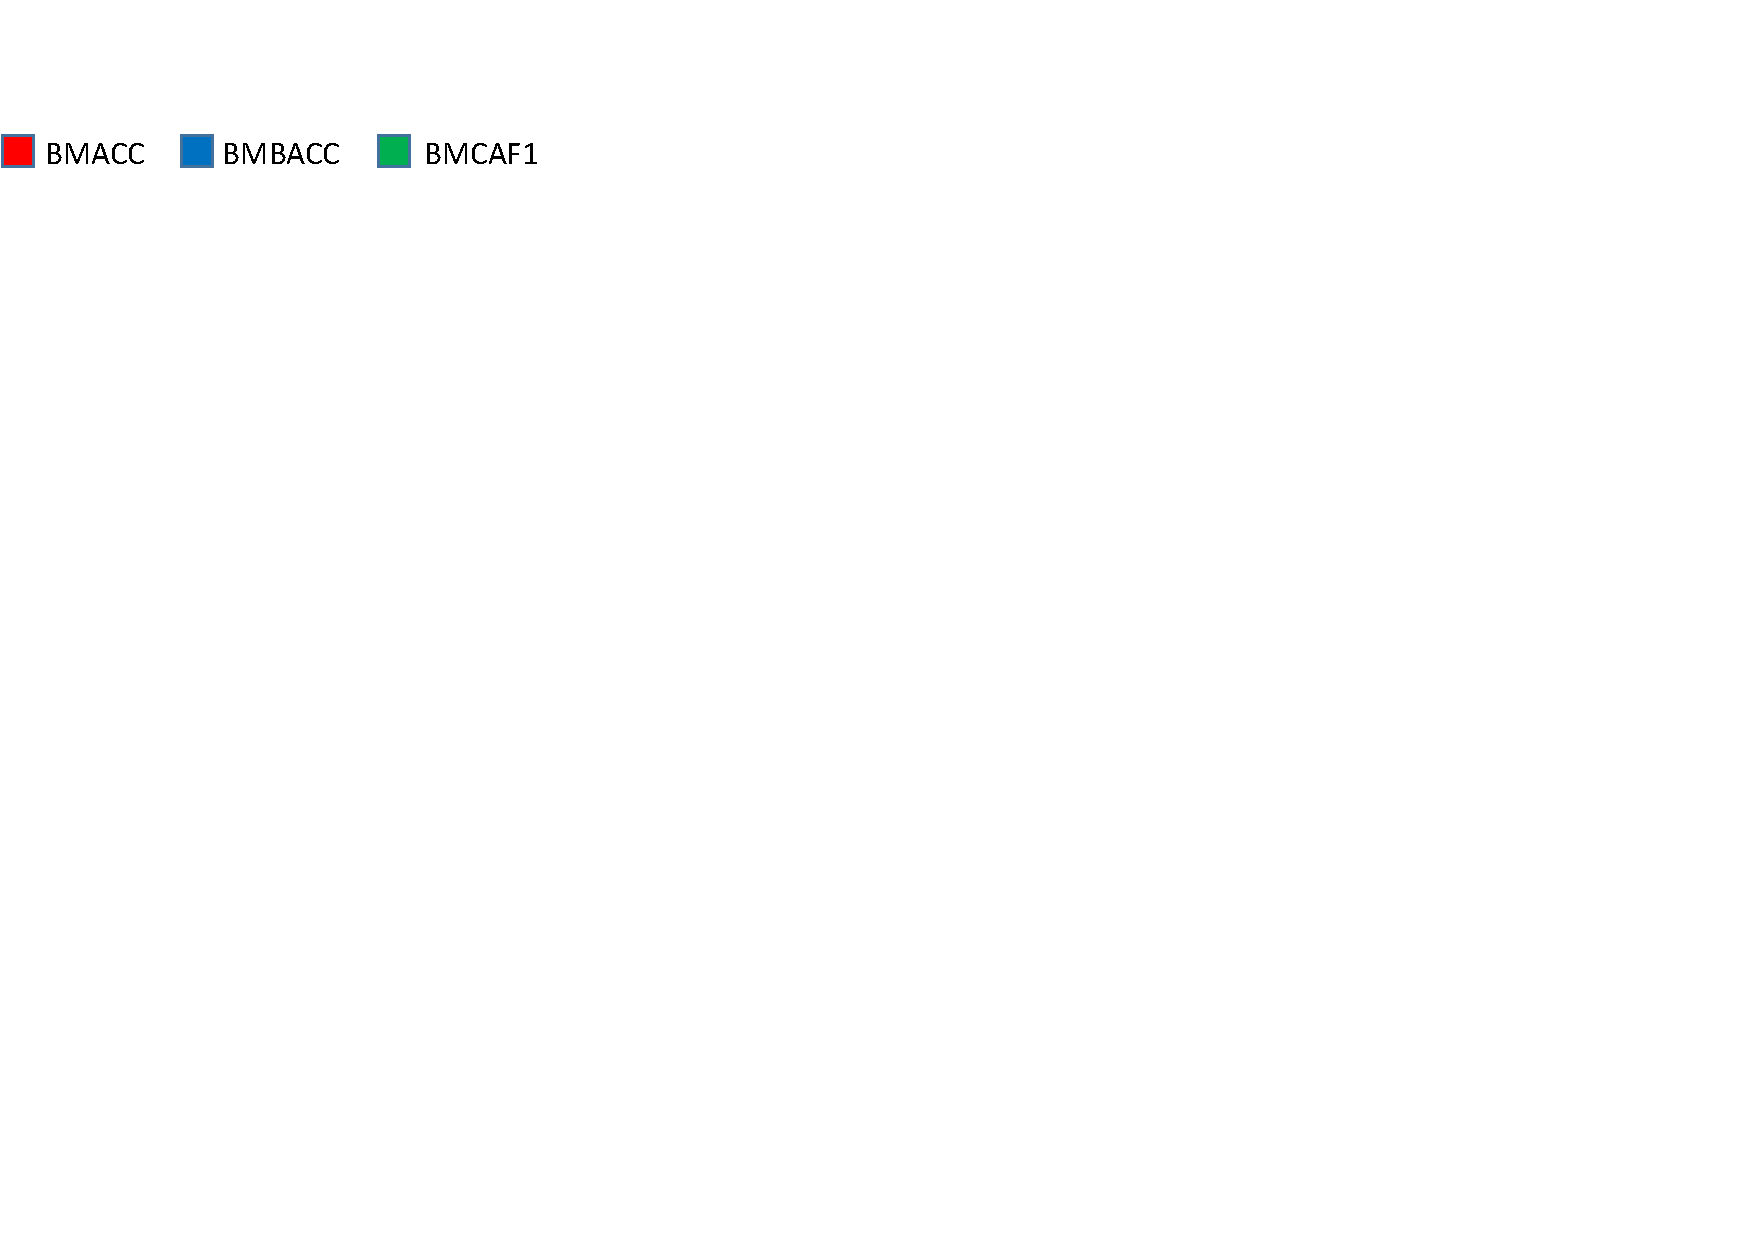
\includegraphics[scale=0.25,trim=0 550 0 0]{./picture/alpha_fig_ledgend.pdf}
	\subfigure[$\delta=1$]{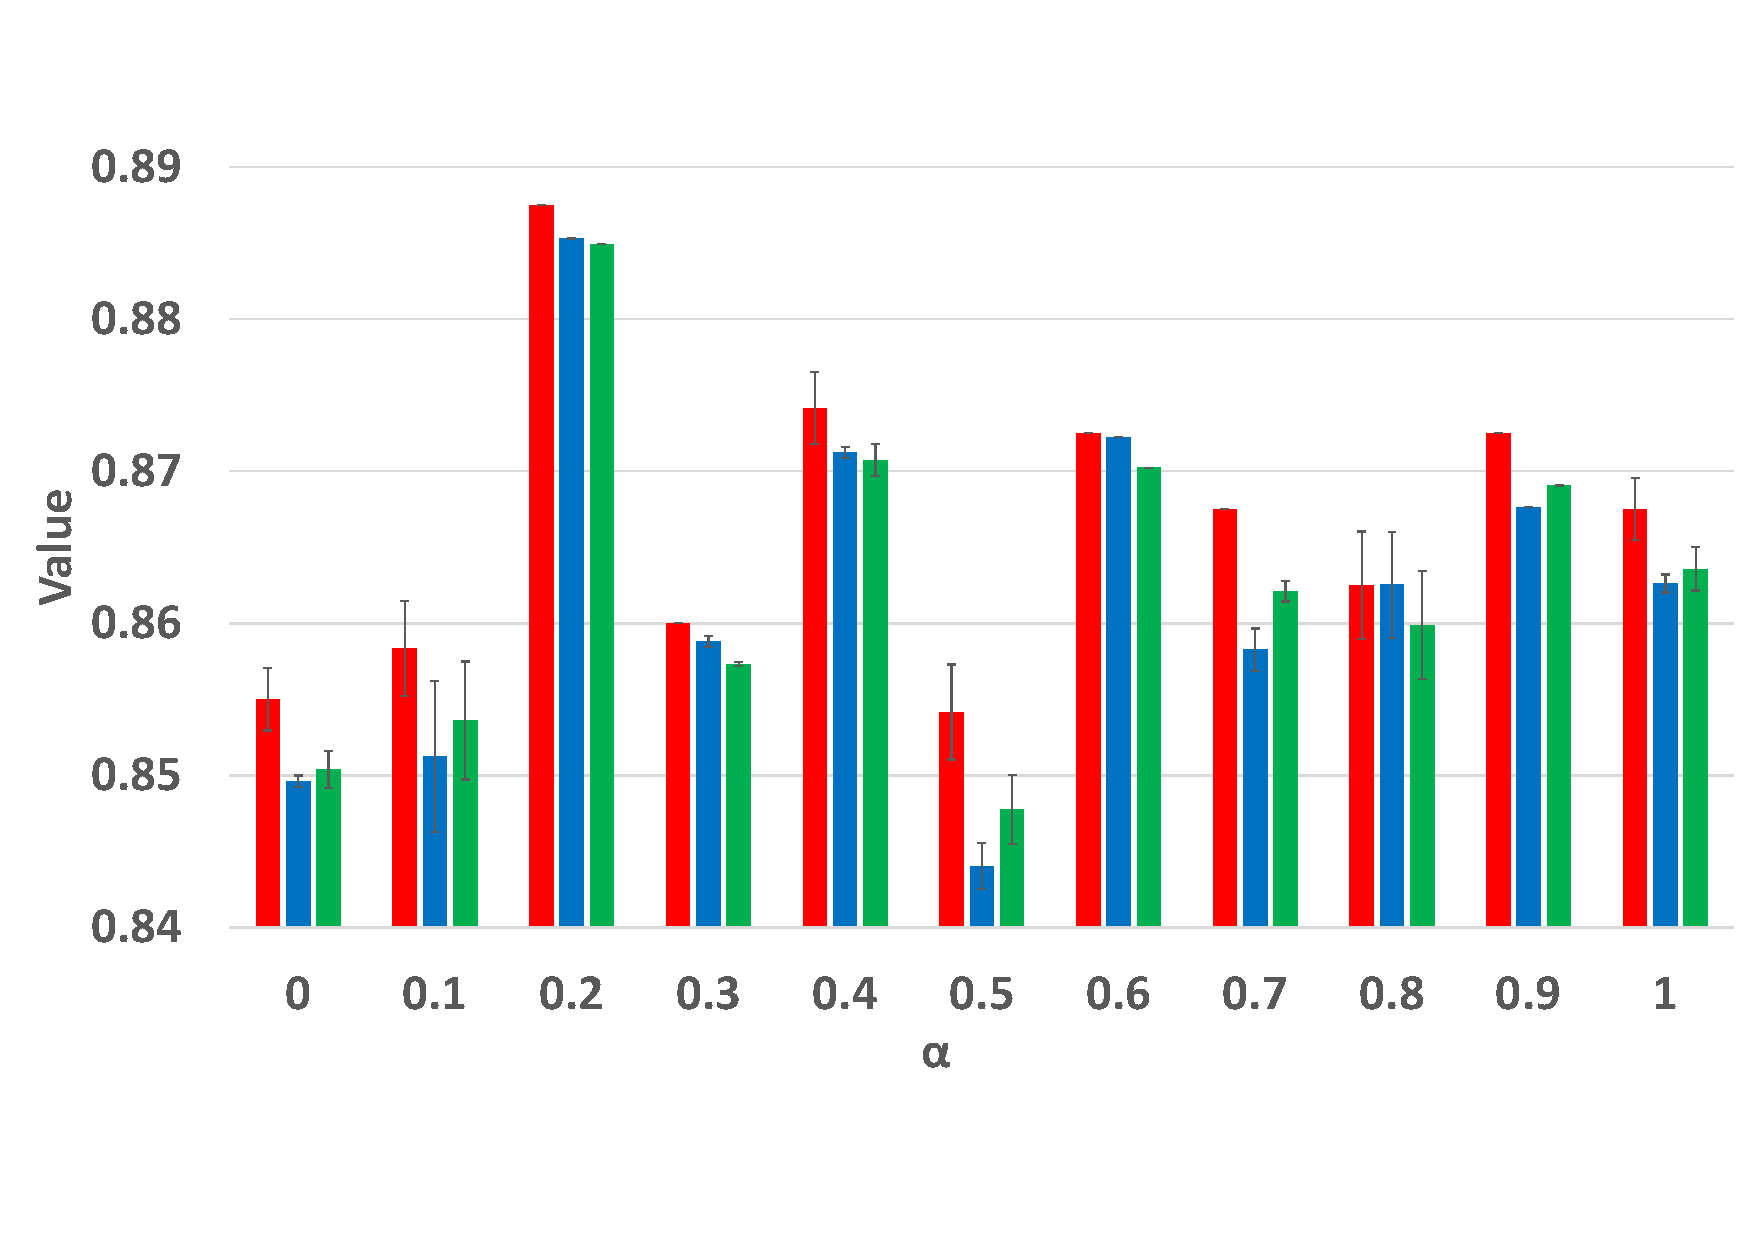
\includegraphics[scale=0.14]{./picture/delta1_alpha.pdf}}
	\subfigure[$\delta=2$]{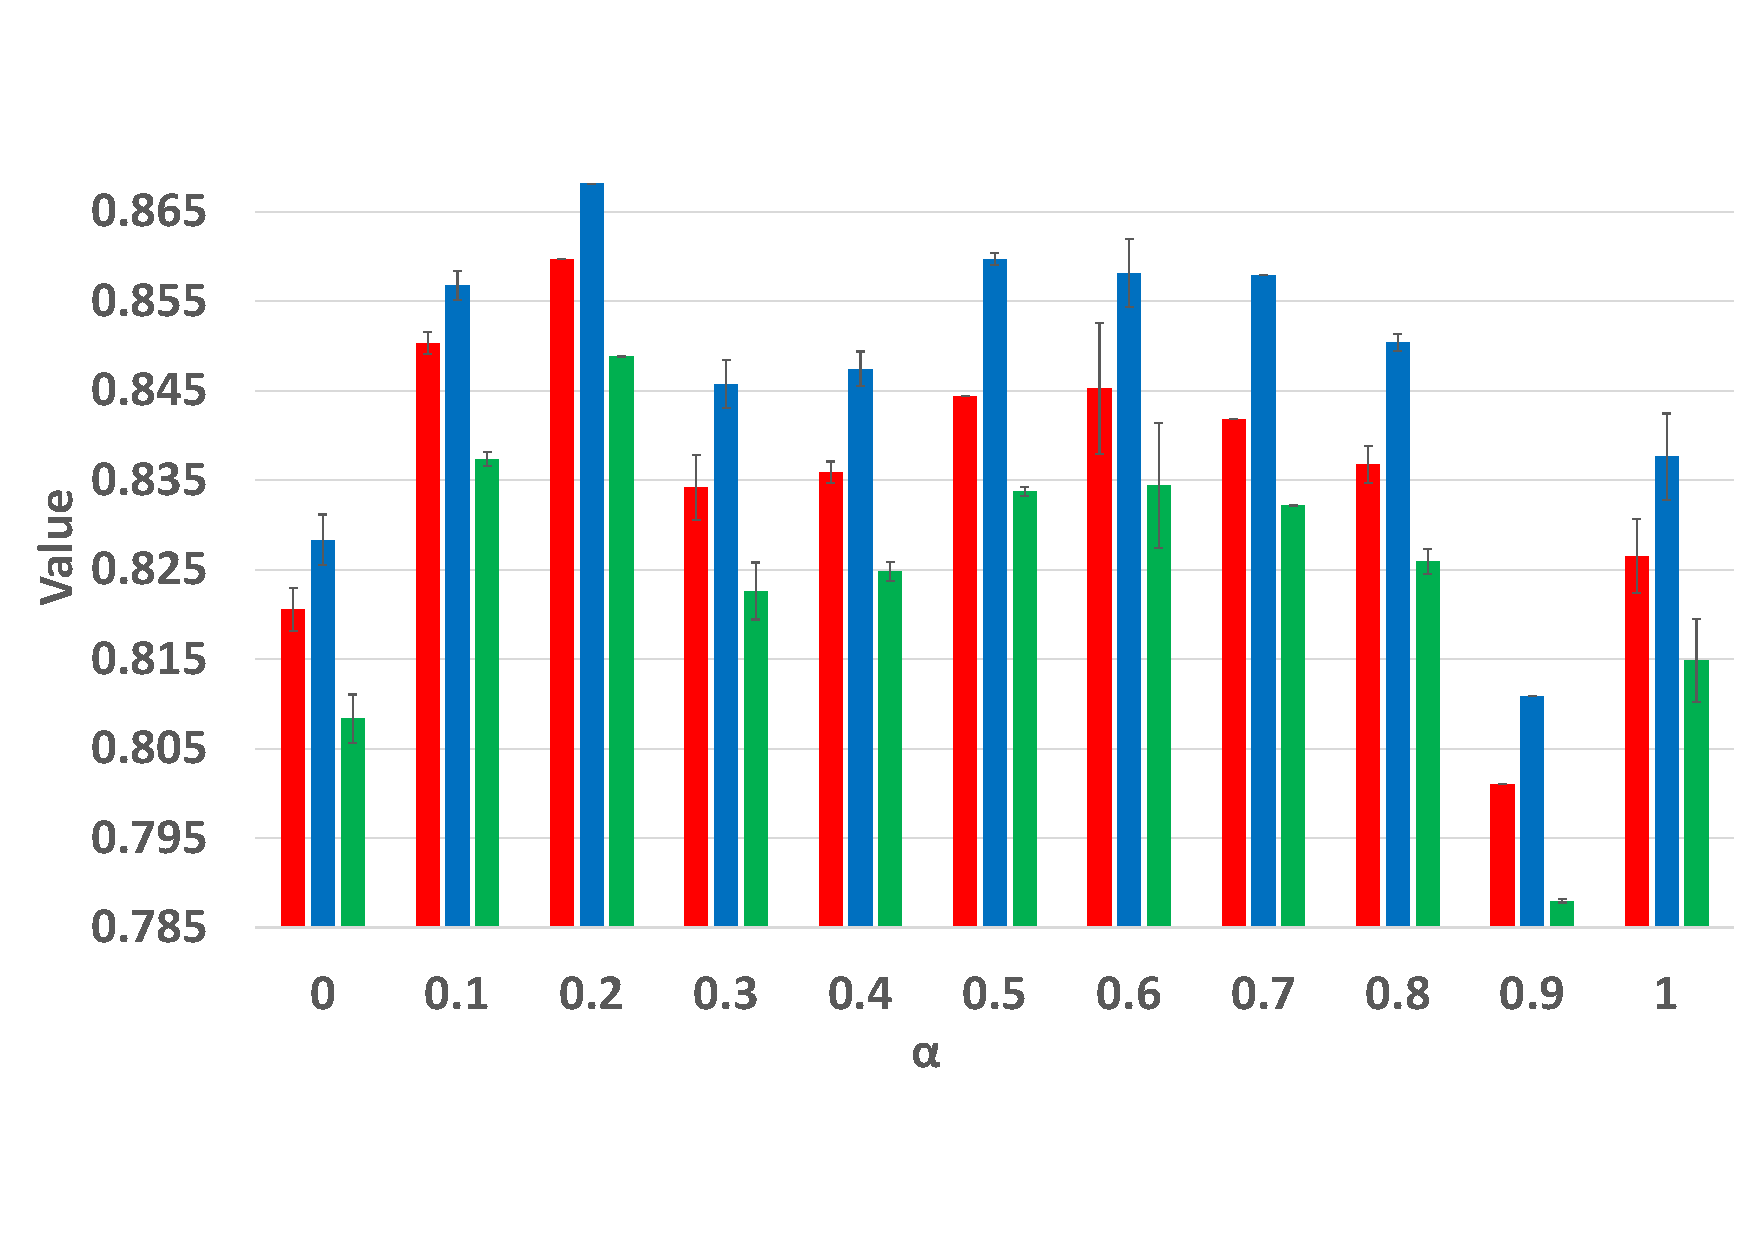
\includegraphics[scale=0.14]{./picture/delta2_alpha.pdf}}
	\subfigure[$\delta=4$]{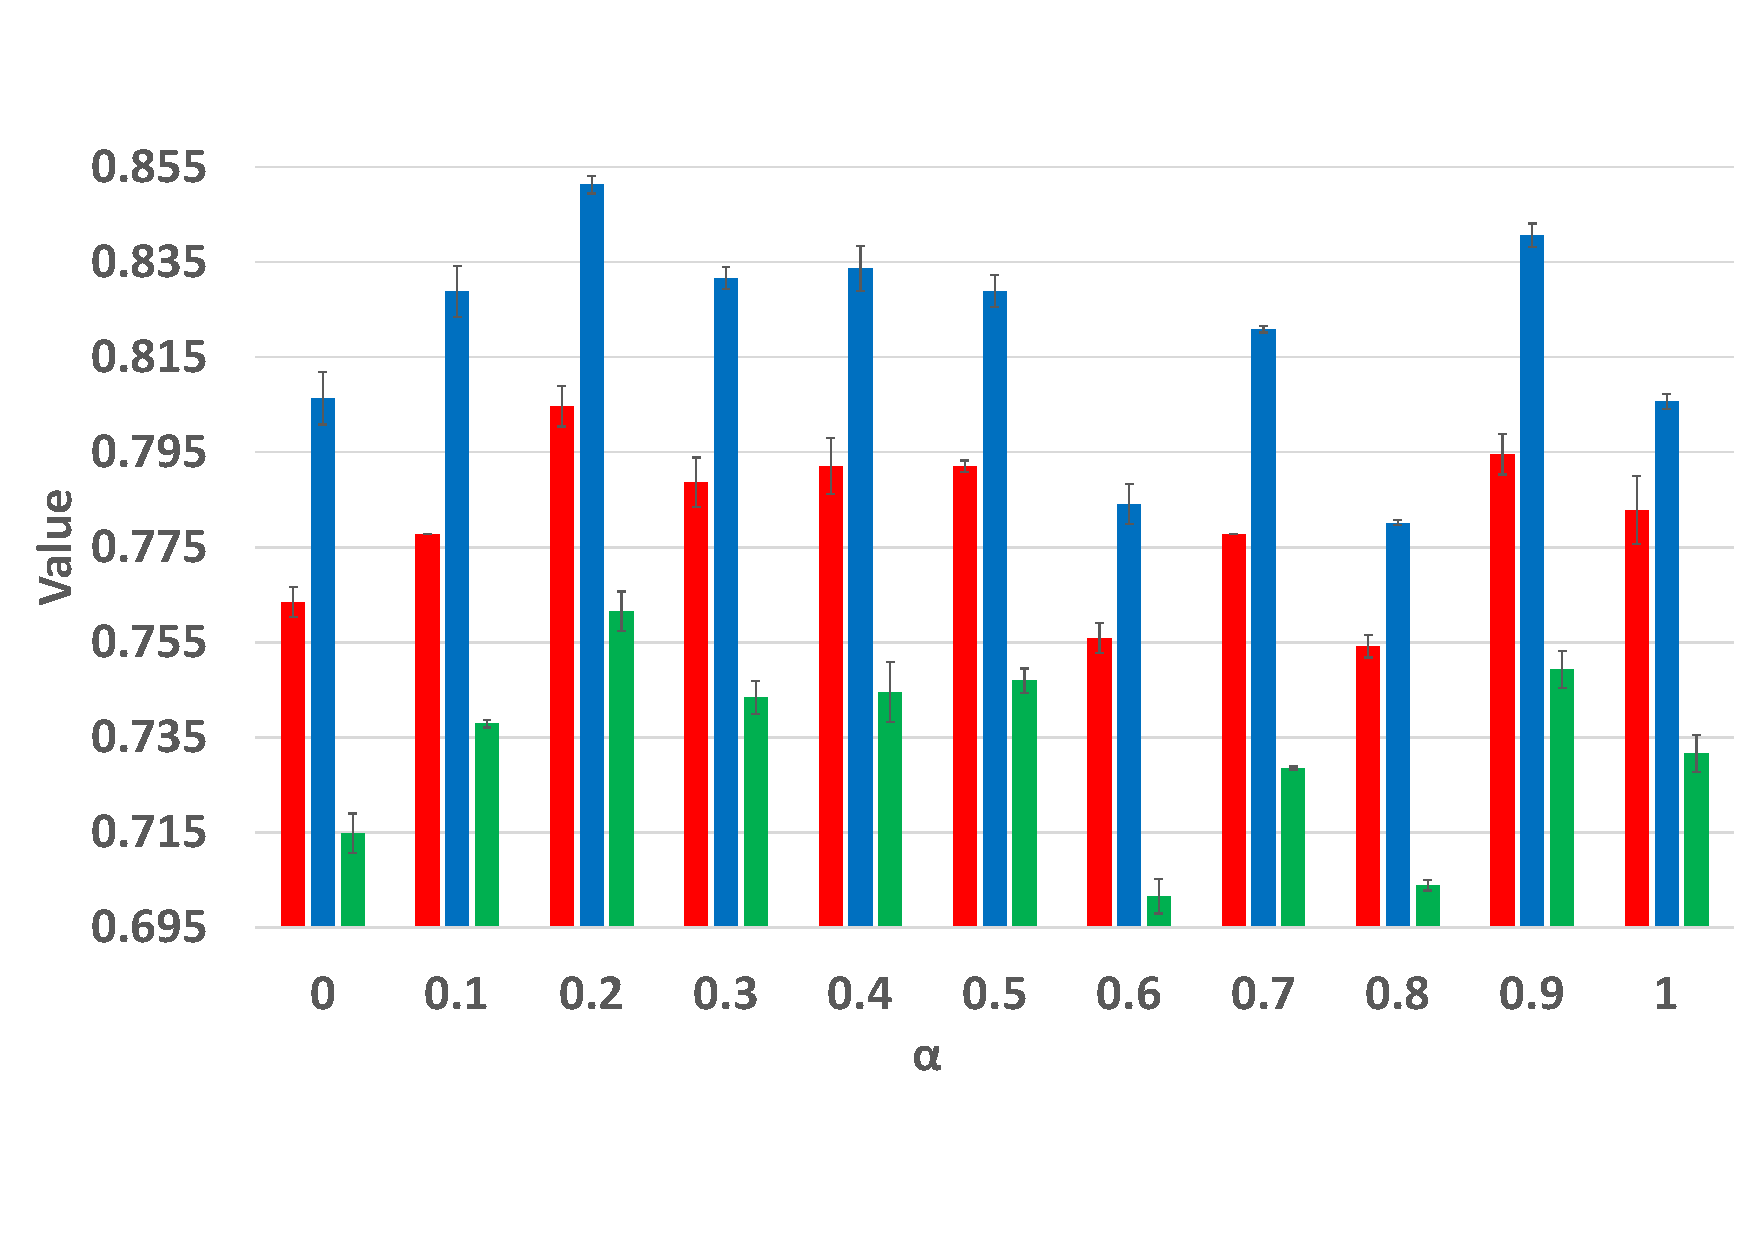
\includegraphics[scale=0.14]{./picture/delta4_alpha.pdf}}
	\subfigure[$\delta=7$]{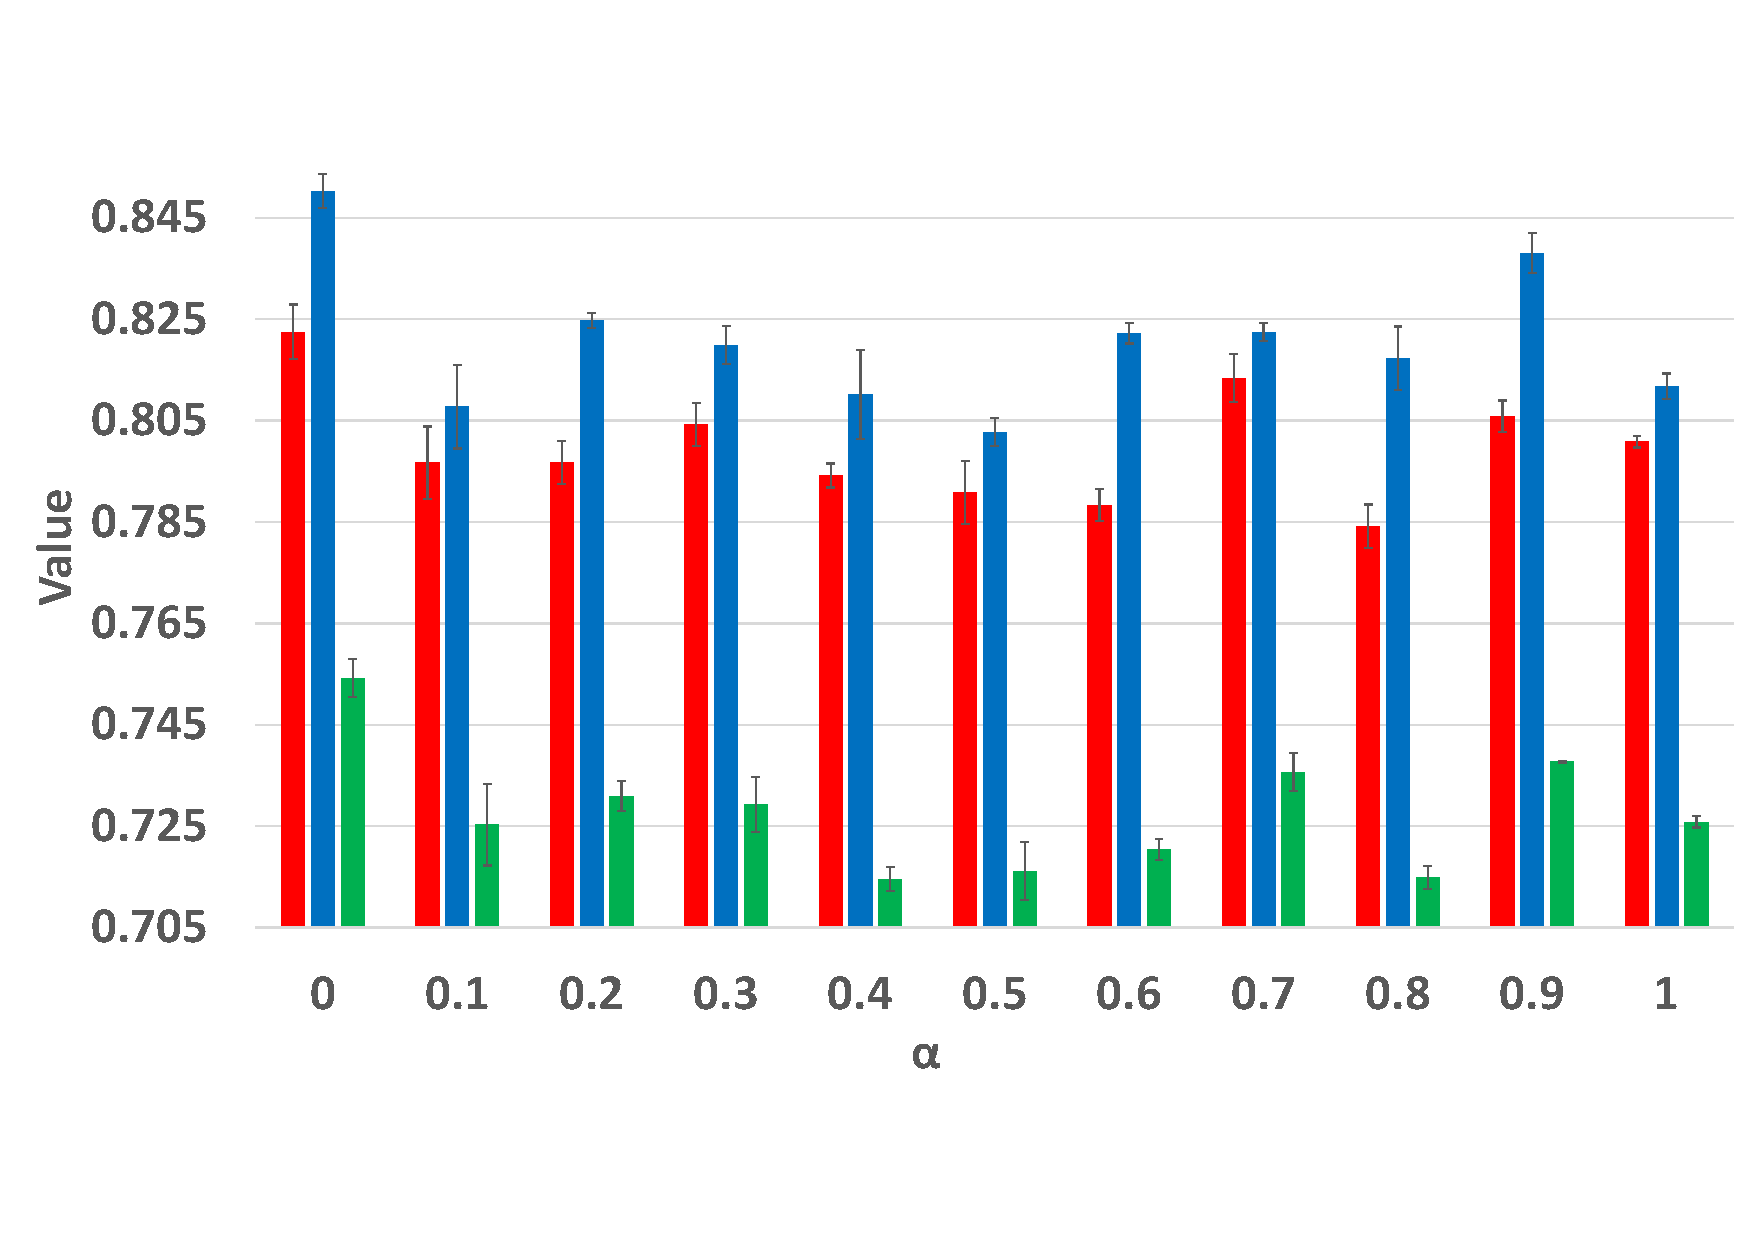
\includegraphics[scale=0.14]{./picture/delta7_alpha.pdf}}
	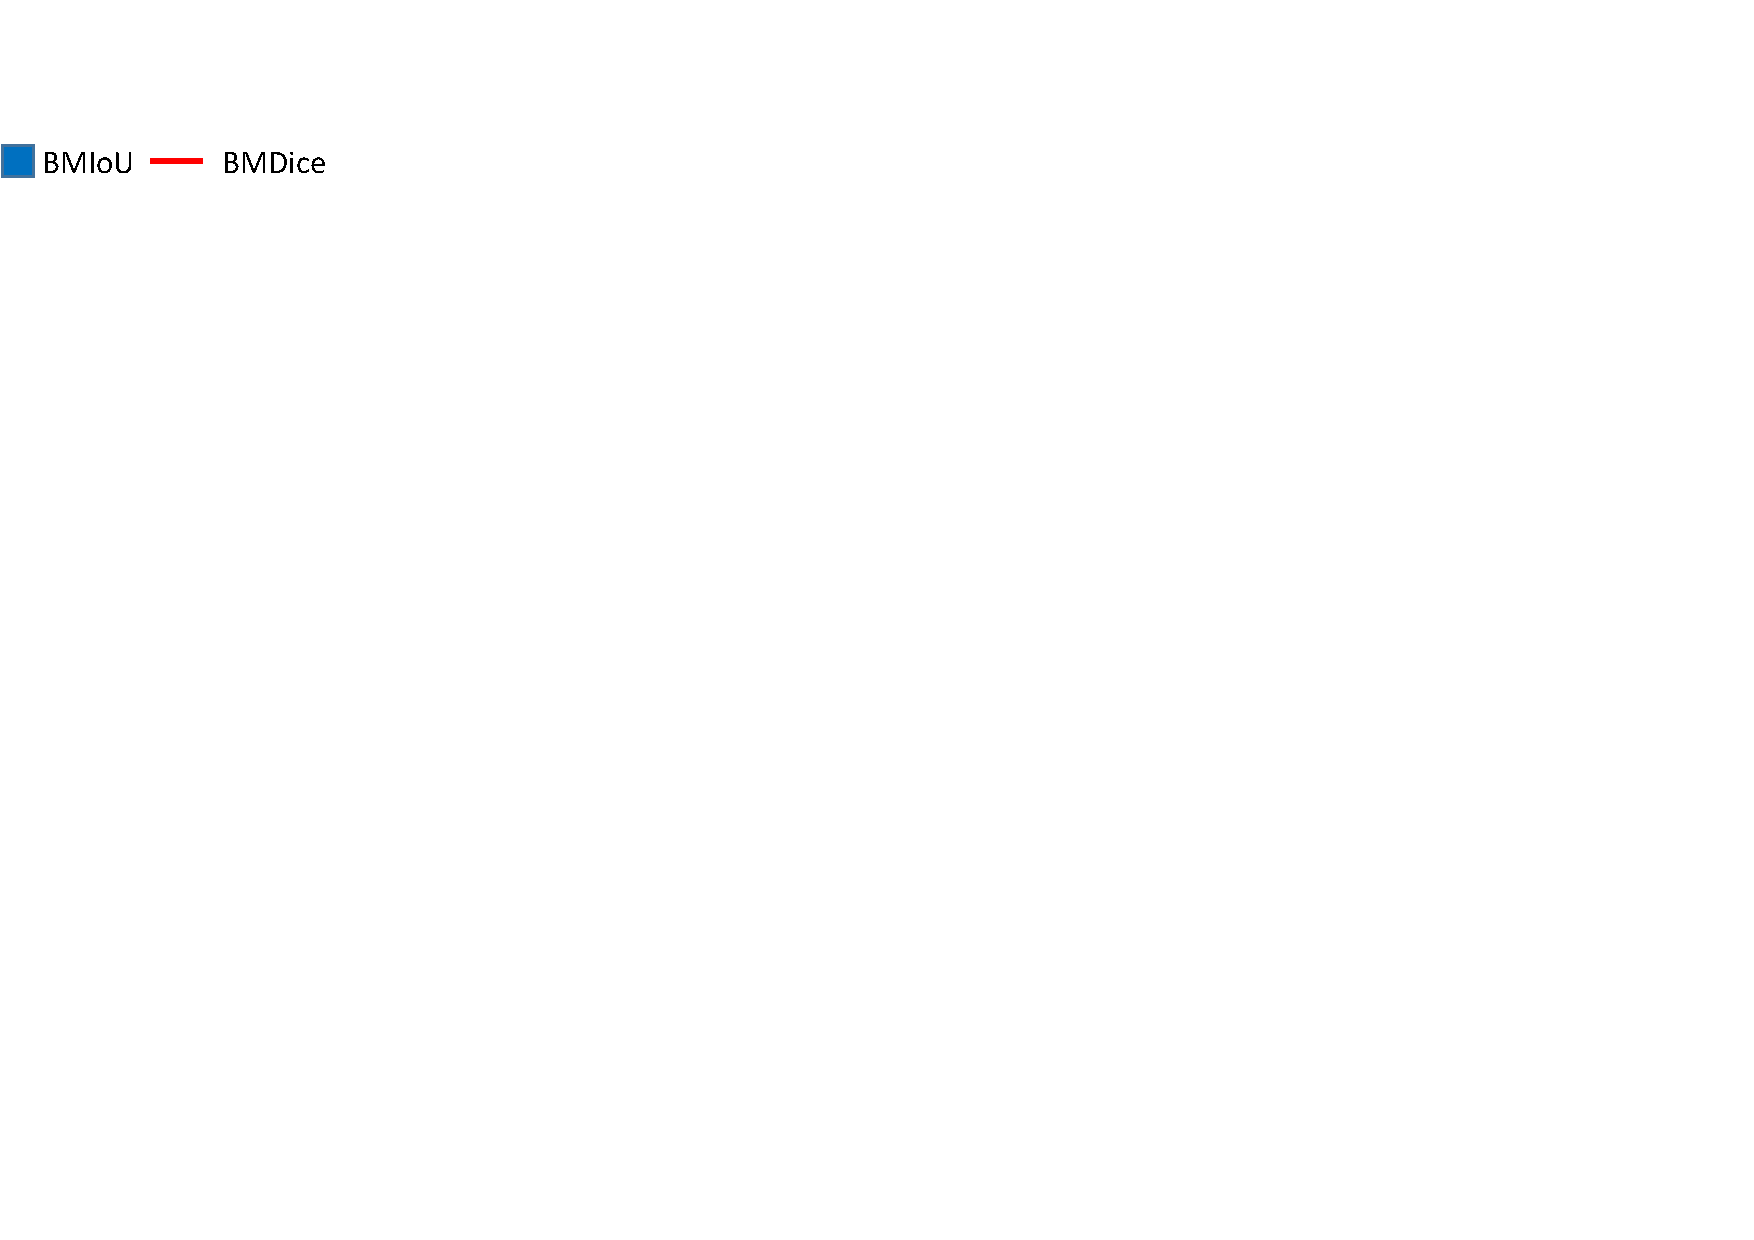
\includegraphics[scale=0.25,trim=0 550 0 0]{./picture/alpha_fig_unet_ledgend.pdf}
	\subfigure[$l=0$]{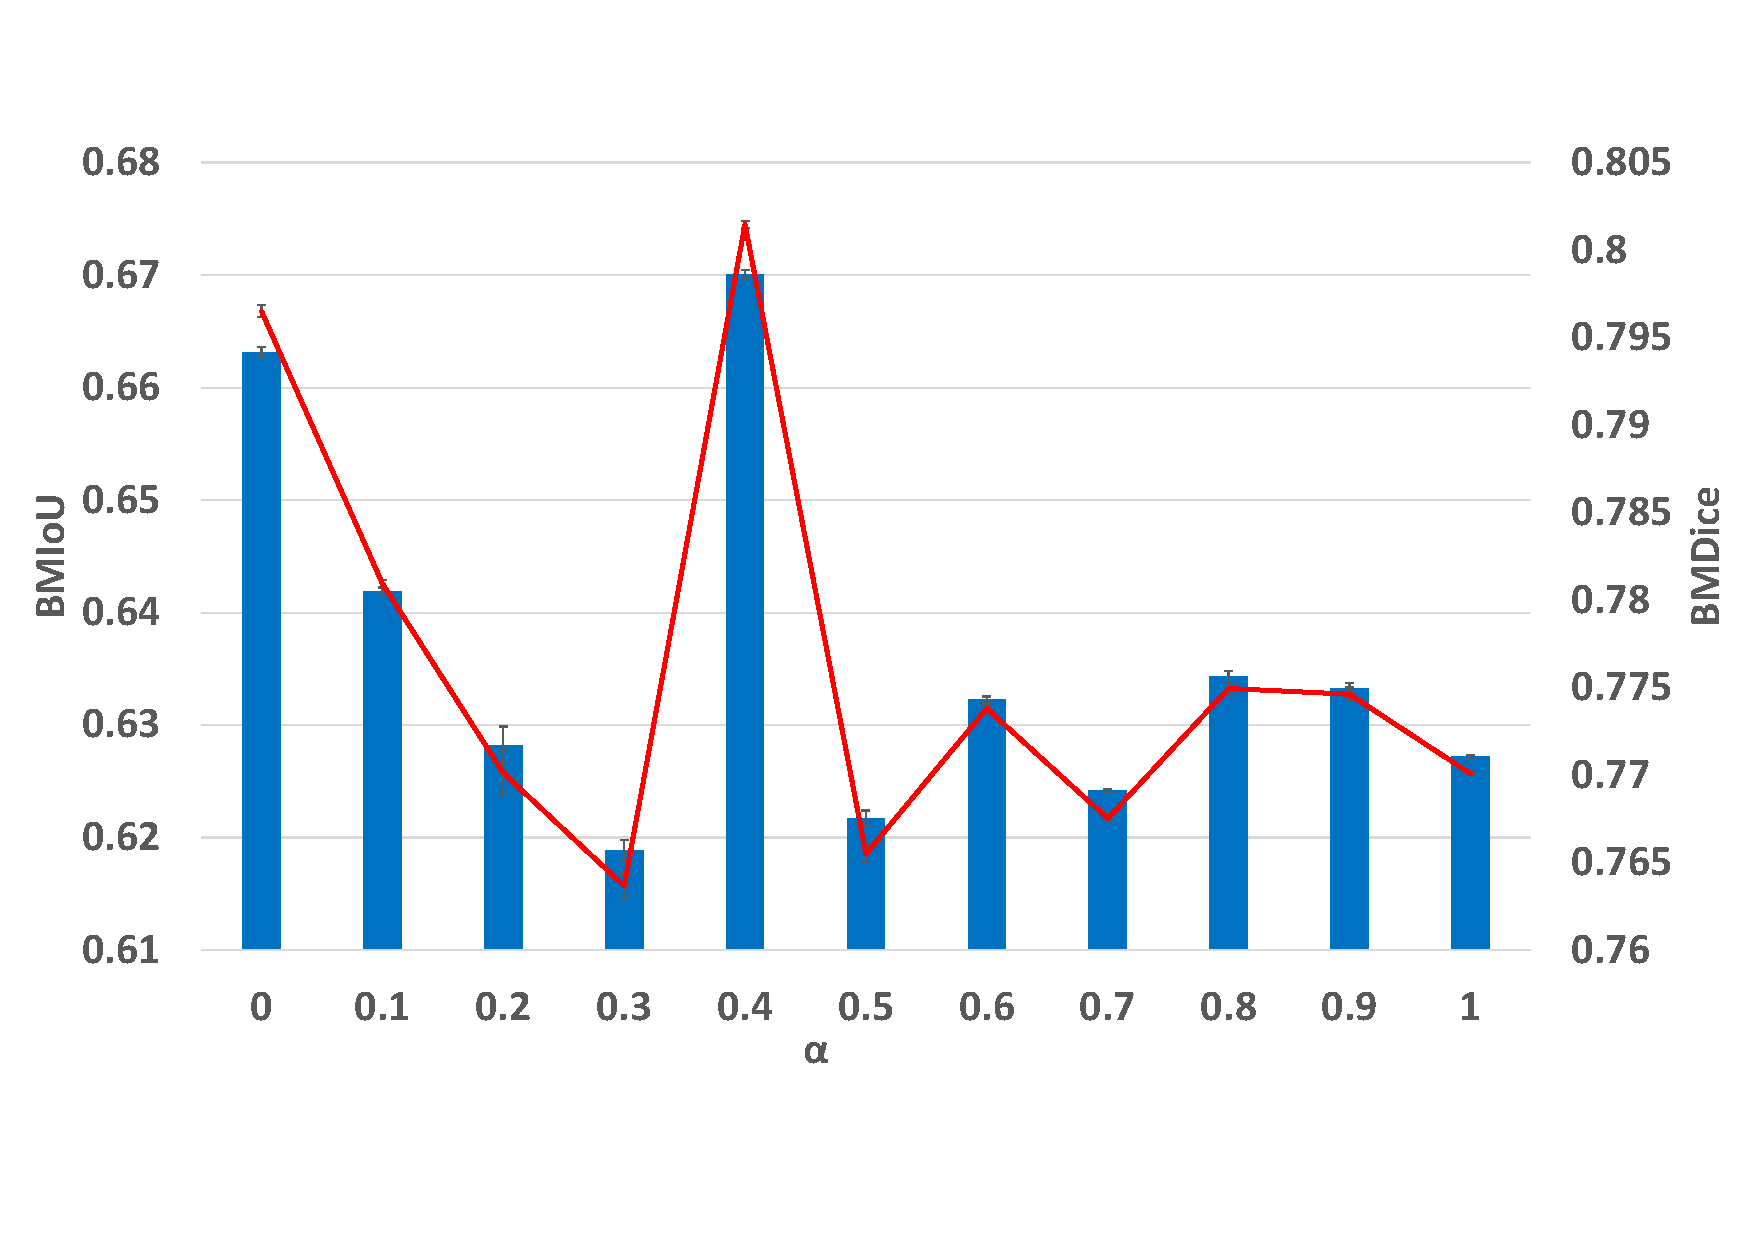
\includegraphics[scale=0.14]{./picture/lack0_alpha.pdf}}
	\subfigure[$l=1$]{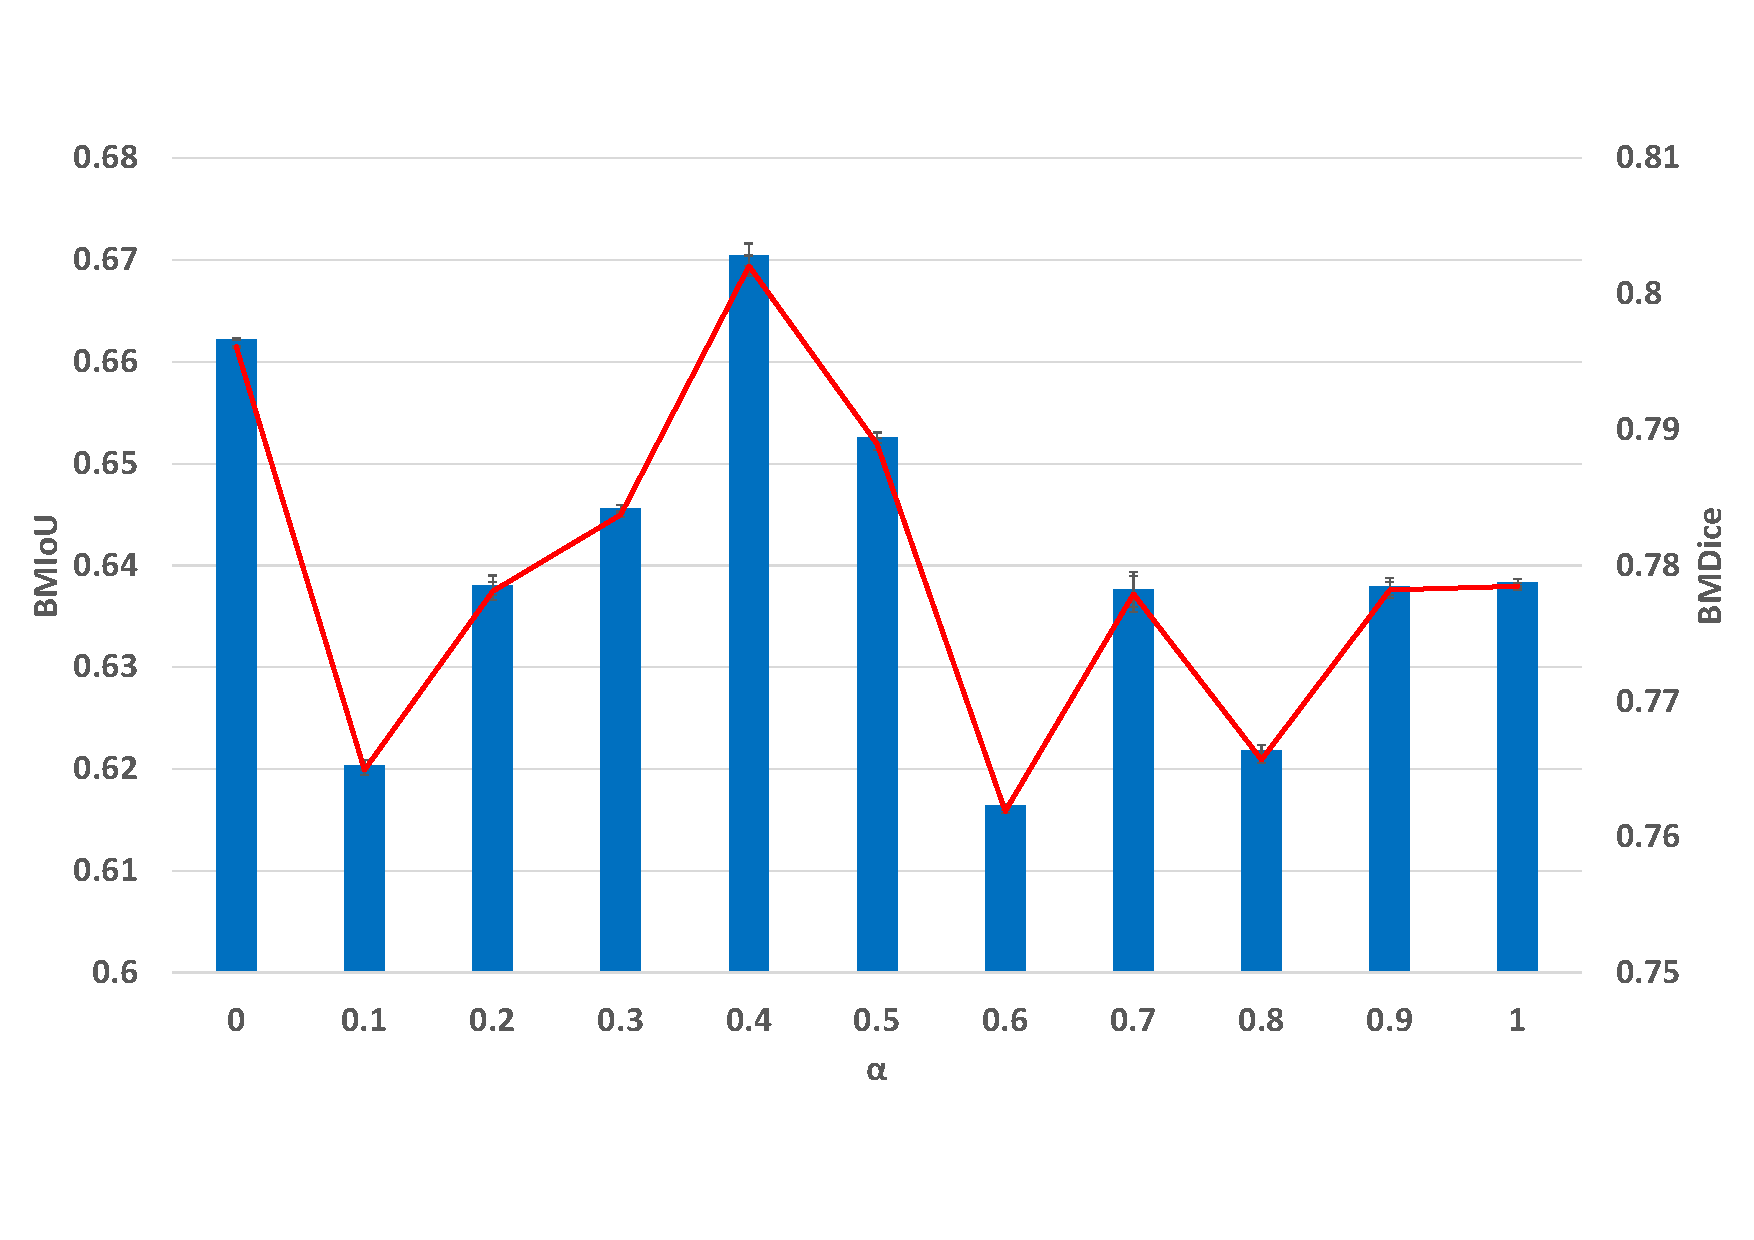
\includegraphics[scale=0.14]{./picture/lack1_alpha.pdf}}
	\subfigure[$l=2$]{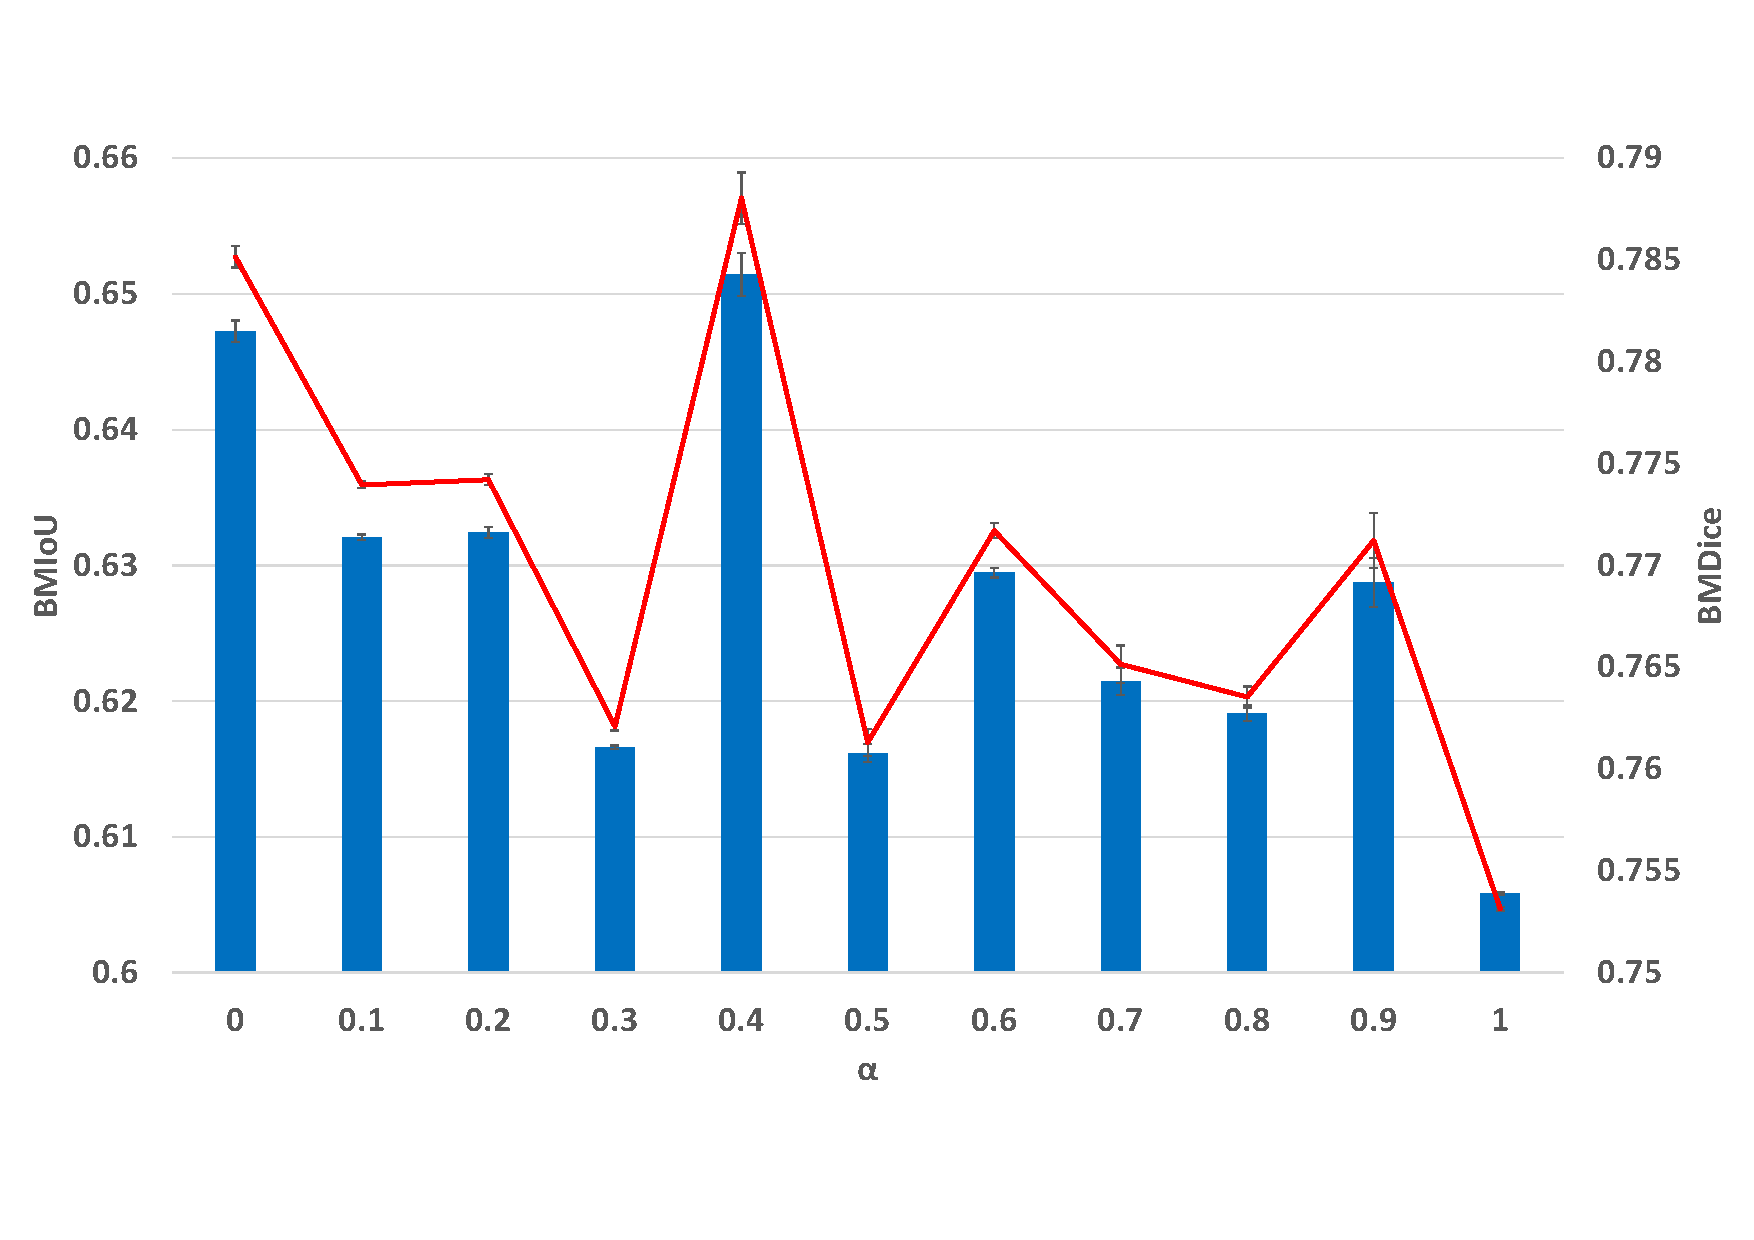
\includegraphics[scale=0.14]{./picture/lack2_alpha.pdf}}
	\subfigure[$l=3$]{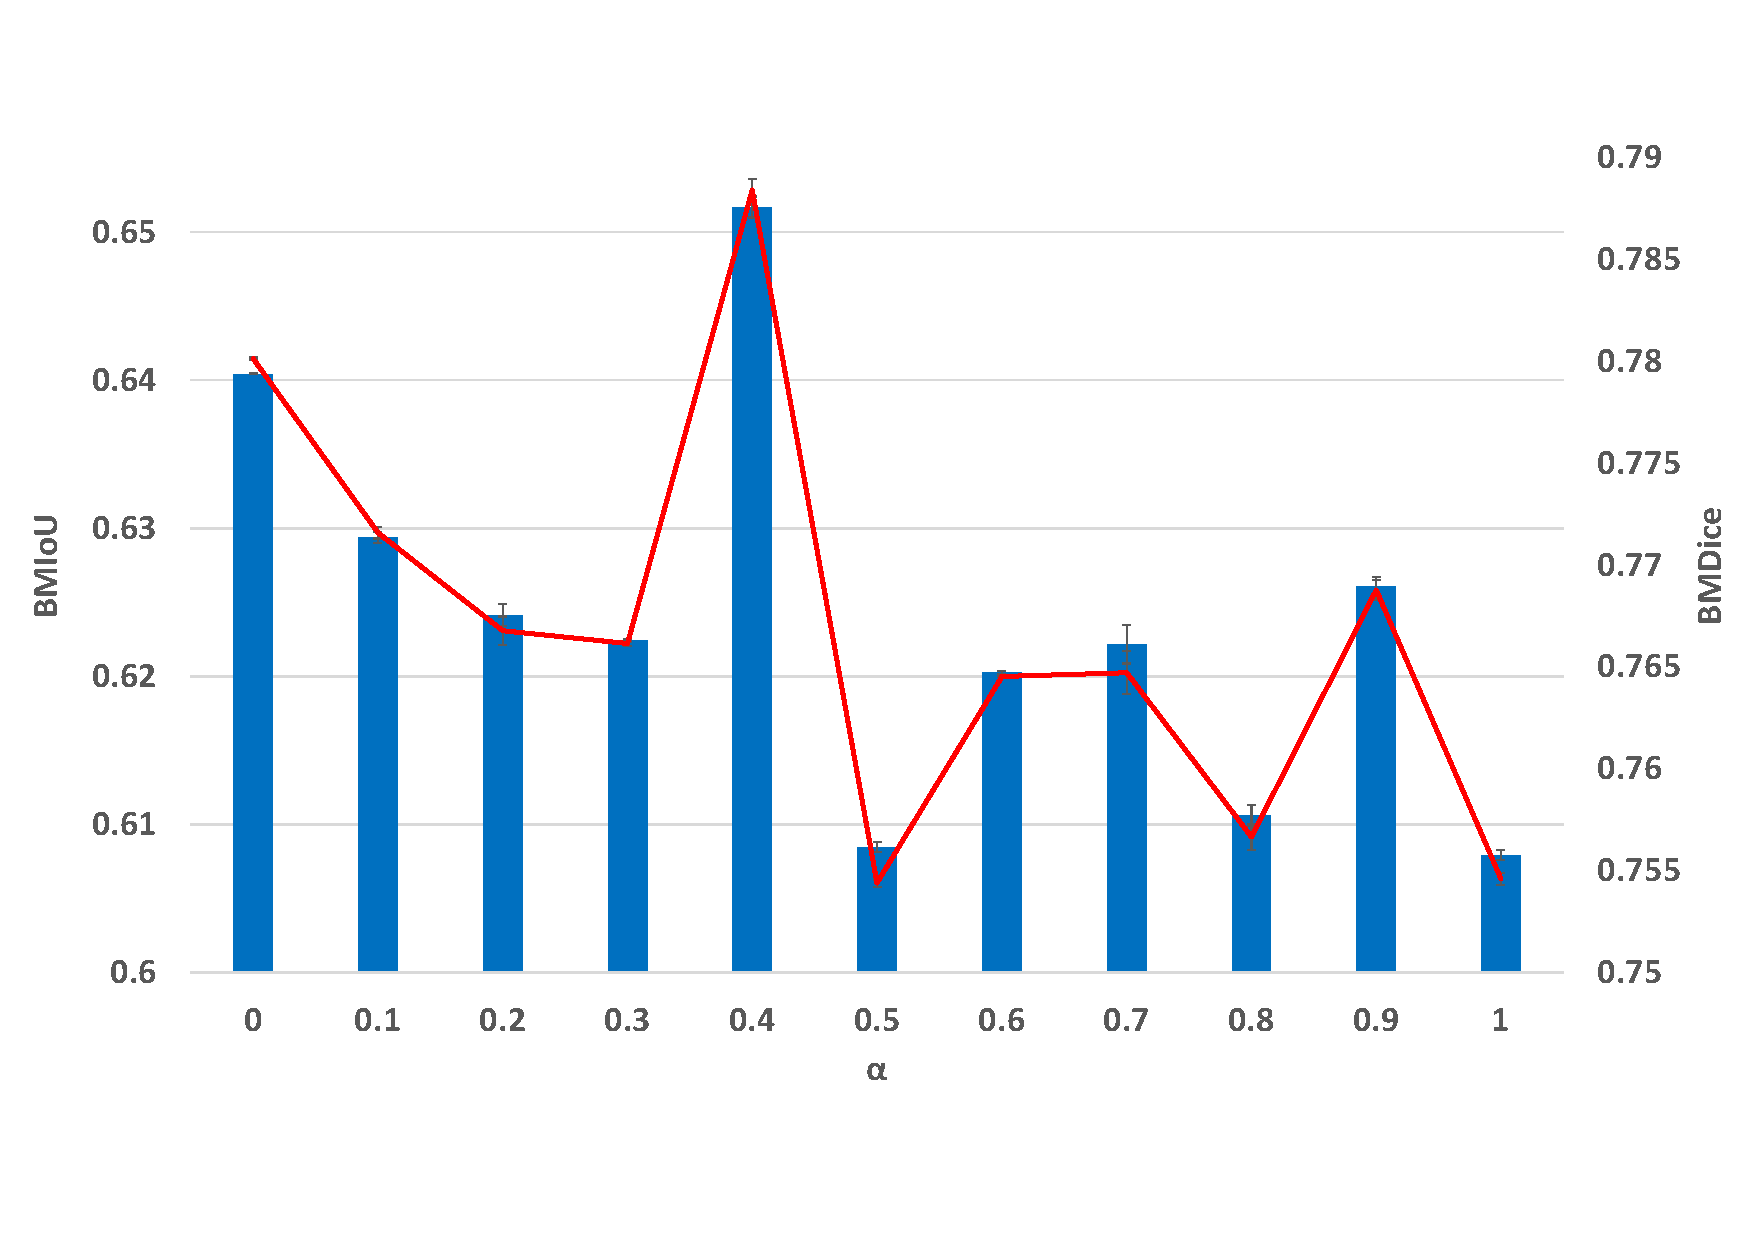
\includegraphics[scale=0.14]{./picture/lack3_alpha.pdf}}
	\caption{\textbf{Result on features calibrating}. Calibrating the multi-encoder's outputs is benefit to improve the model's accuracy after aggregating. Sub-fig (a) to (d) are classification task training by LUNA16 and (e) to (h) are segmentation task training by BraTS 2017. Despite the different distribute of data, optimal value is near to $\alpha=0.2$ in LUNA16 and $\alpha=0.4$ in BraTS 2017.}
	\label{fig_alpha_result}
\end{figure}


\begin{figure}
	\centering
	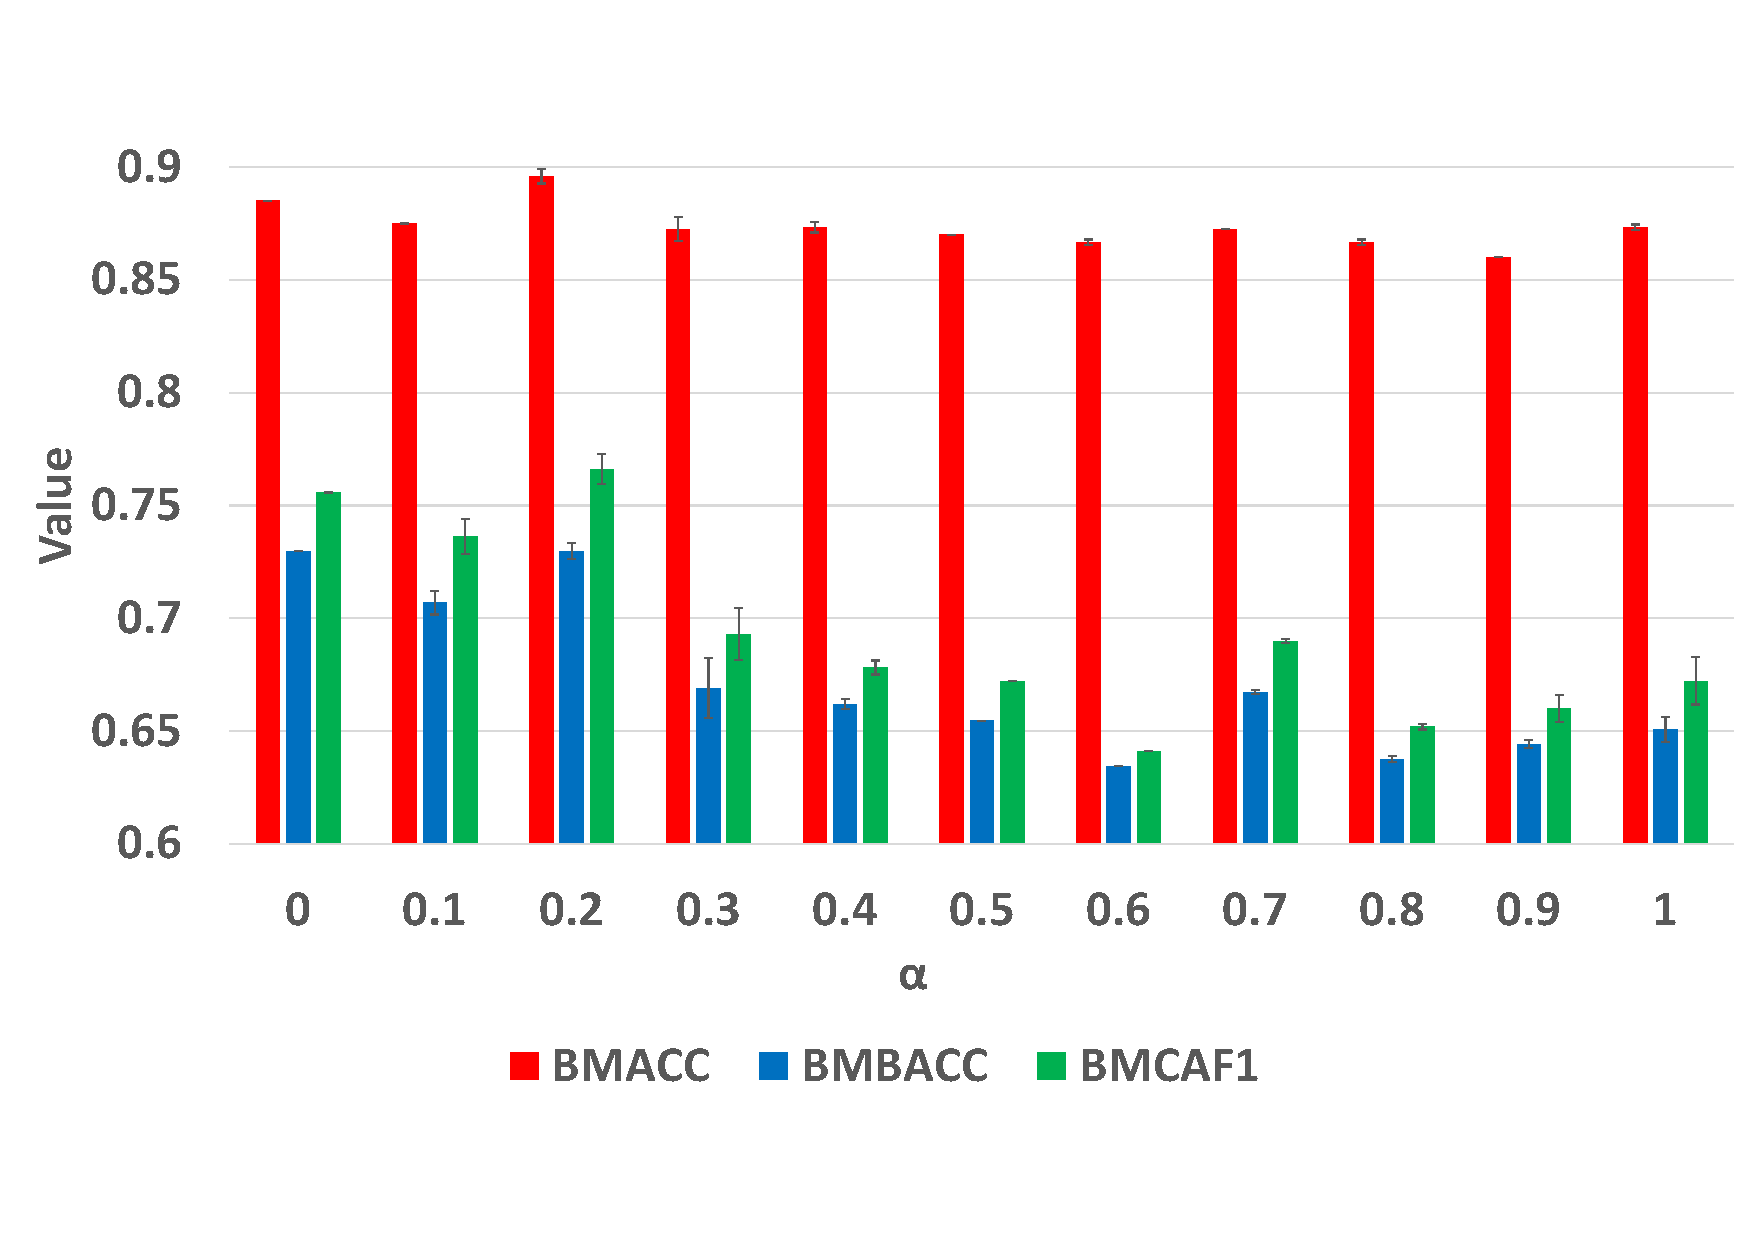
\includegraphics[scale=0.25]{./picture/delta7_alpha_add.pdf}
	\caption{\textbf{Complement experiment when $\delta=7$}. We add another experiment on LUNA16 when $\delta=7$ and $\lambda=100$. The result shows that the optimal coefficient value is $\aleph=0.2$.}
	\label{fig_delta7_alpha_add}
\end{figure}


\subsection{Result on personalized aggregating}
From the Equation \ref{divergence_aggregate}, we can analyze that if $\lambda x>1$, $x$ should be considered as personalizing parameter when the select function $g=e^{-(\lambda x)^{\gamma}}$ and $\gamma=+\infty$. Thus, the number of personalizing parameters and $\lambda$ should be in direct ratio. In this paper we fixed $\gamma$ as 10. And we defined that personalizing ratio is the number of parameters' STD which multiplied by $\lambda$ is larger than 1 being divided by the number of total parameters. We used LUNA16 datasets with $\delta=7$ and BraTS 2017 datasets with $l=3$ to validate this assumption.

We got results on Figure \ref{fig_lambda_select_result} which are divided into four sub-figures. Sub-figure (a) and (b) shown personalizing ratio and classifier's parameters' mean STD between different clients in classification task and sub-figure (c) and (d) shown identical metric in segmentation task. The personalizing ratio in classification task presents stepped increase while it increase at first and then decrease in segmentation task. The reason we guessing is that the number of classifier's parameters in classification task is far lower than decoder's in segmentation task. But in total, personalizing ratio increases with $\lambda$ becoming bigger. And we find that there are threshold in $\lambda$ and  personalizing ratio is not zero if $\lambda$ is bigger than it.

\begin{figure}
	\centering
	\subfigure[Classification personalizing rate]{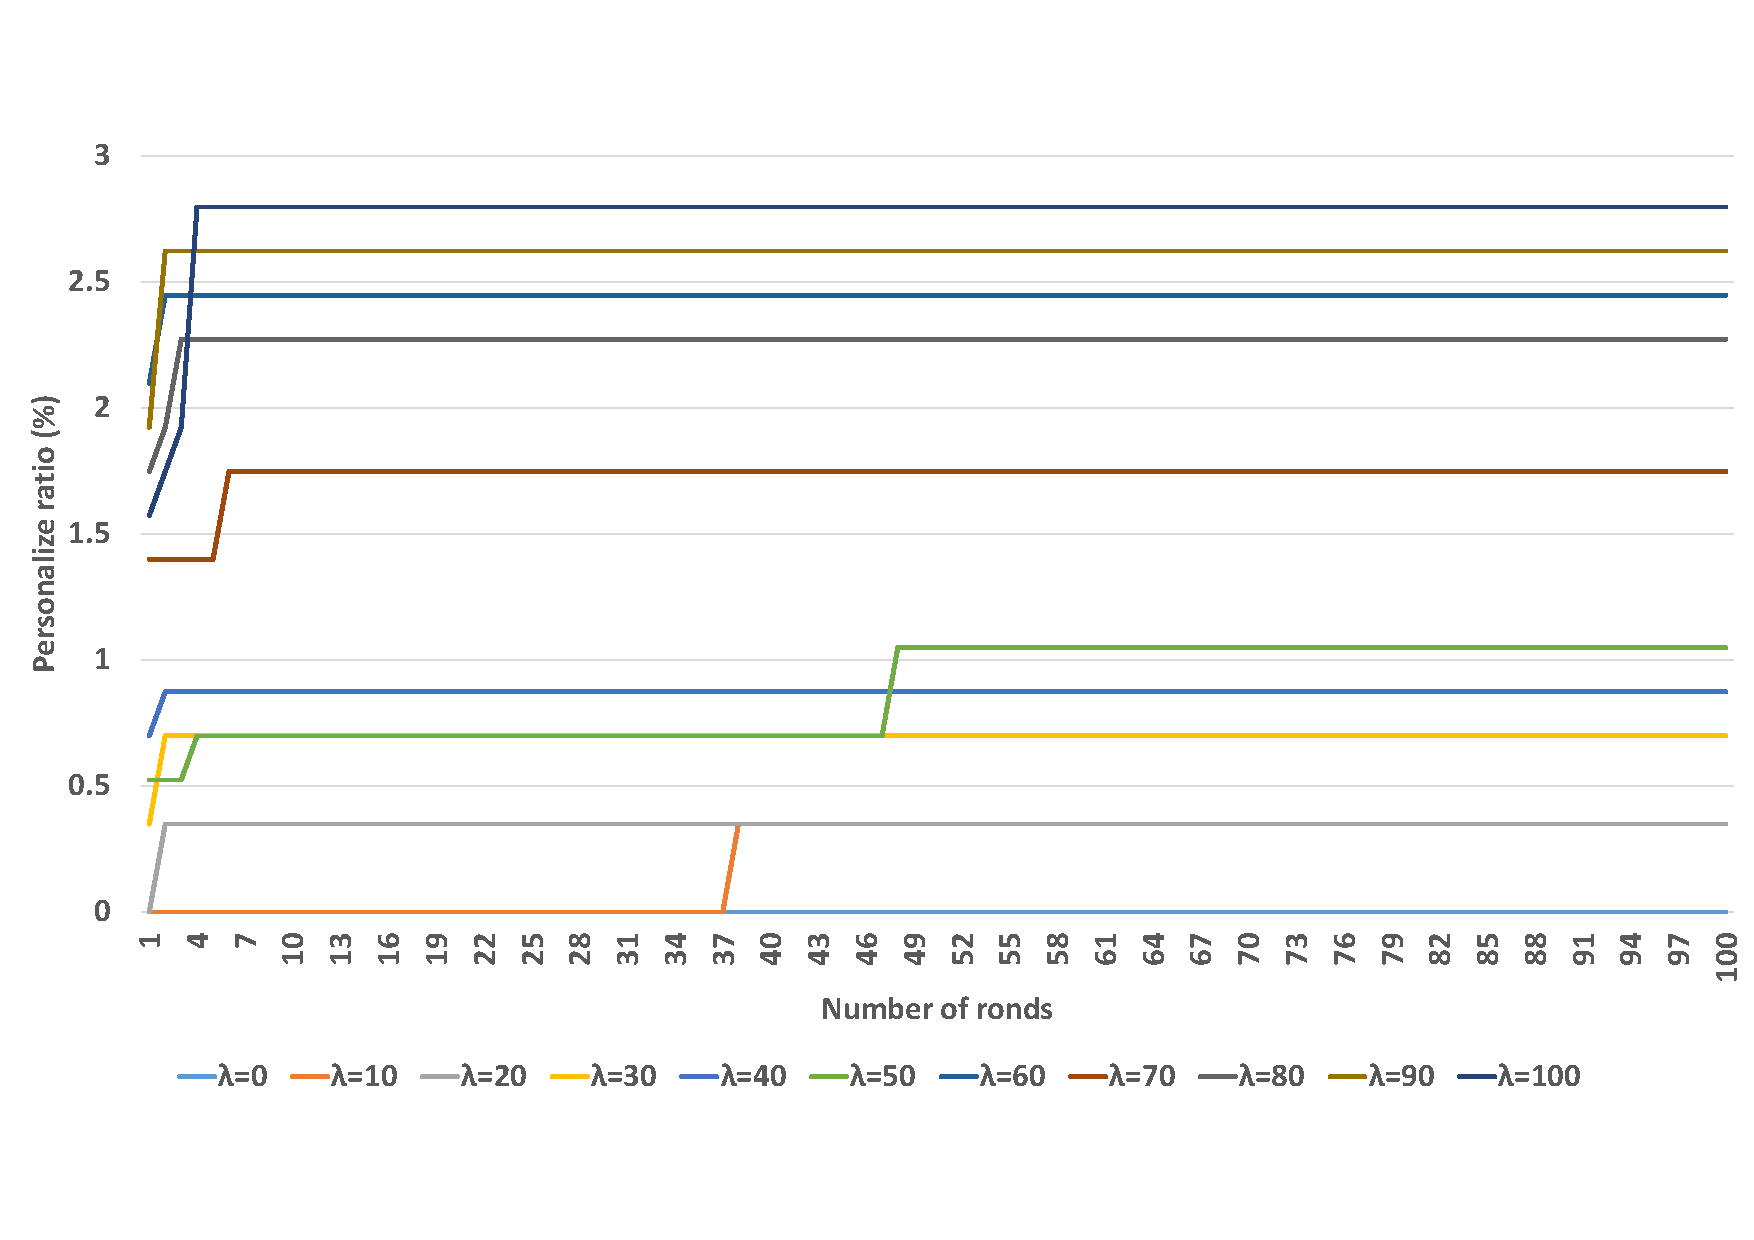
\includegraphics[scale=0.14]{./picture/select_function_luna.pdf}}
	\subfigure[Classification mean std ]{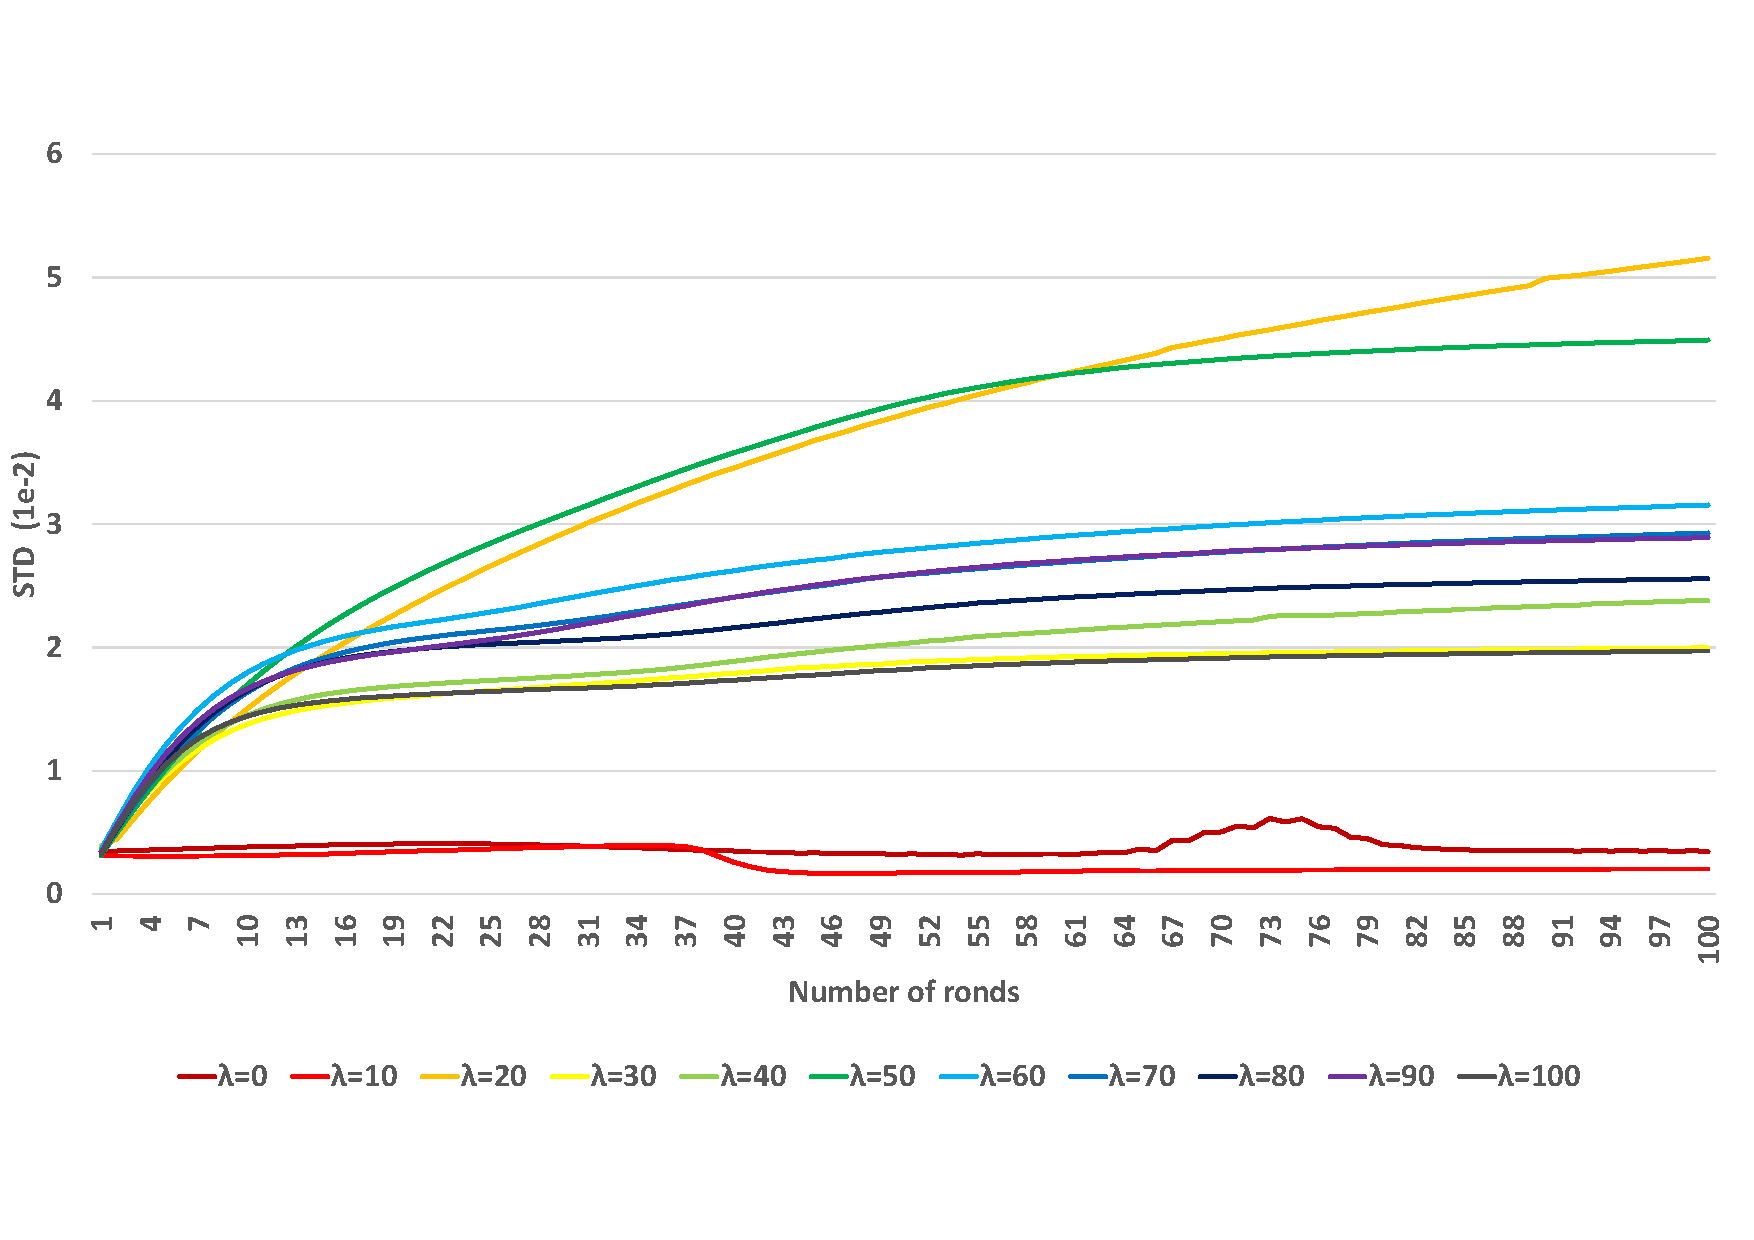
\includegraphics[scale=0.14]{./picture/select_function_luna_std_mean.pdf}}
	\subfigure[Segmentation personalizing rate]{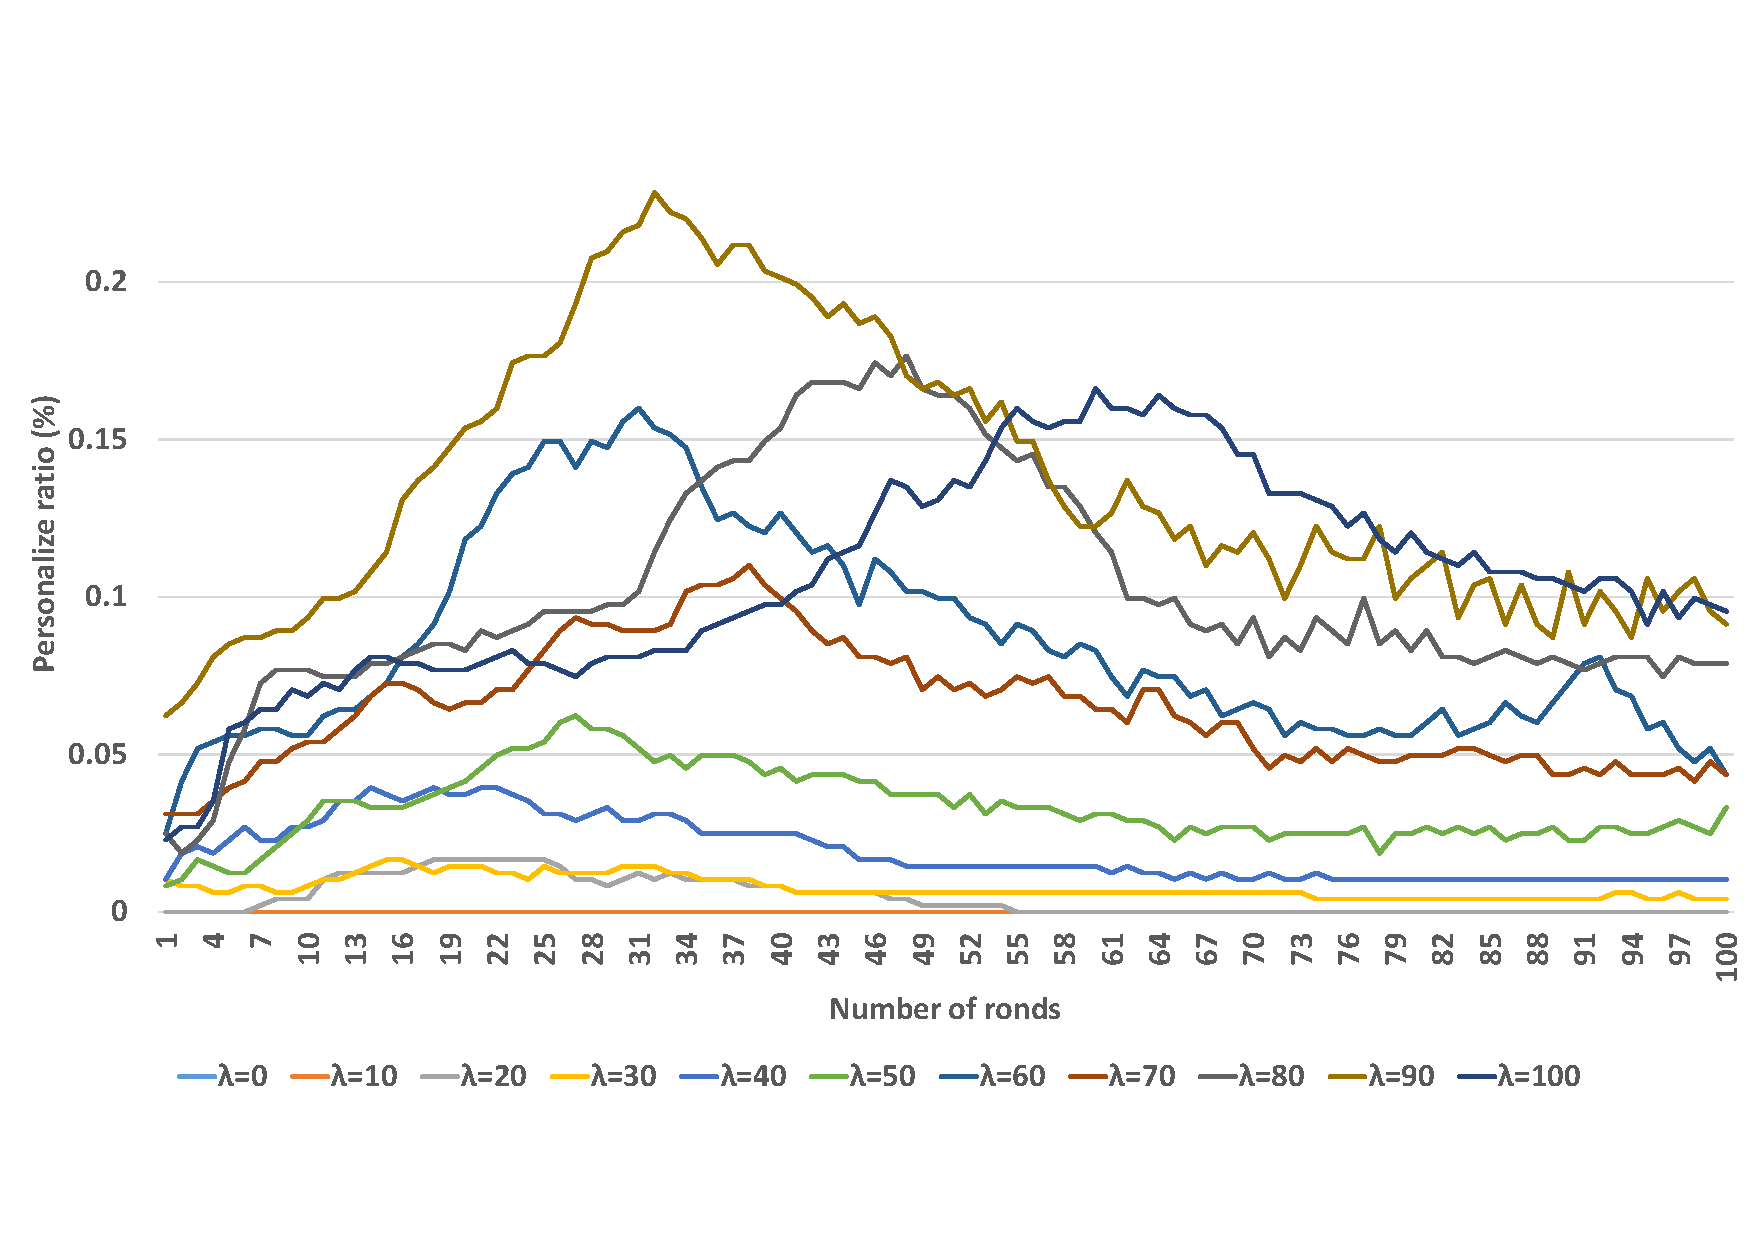
\includegraphics[scale=0.14]{./picture/select_function_unet.pdf}}
	\subfigure[Segmentation mean std]{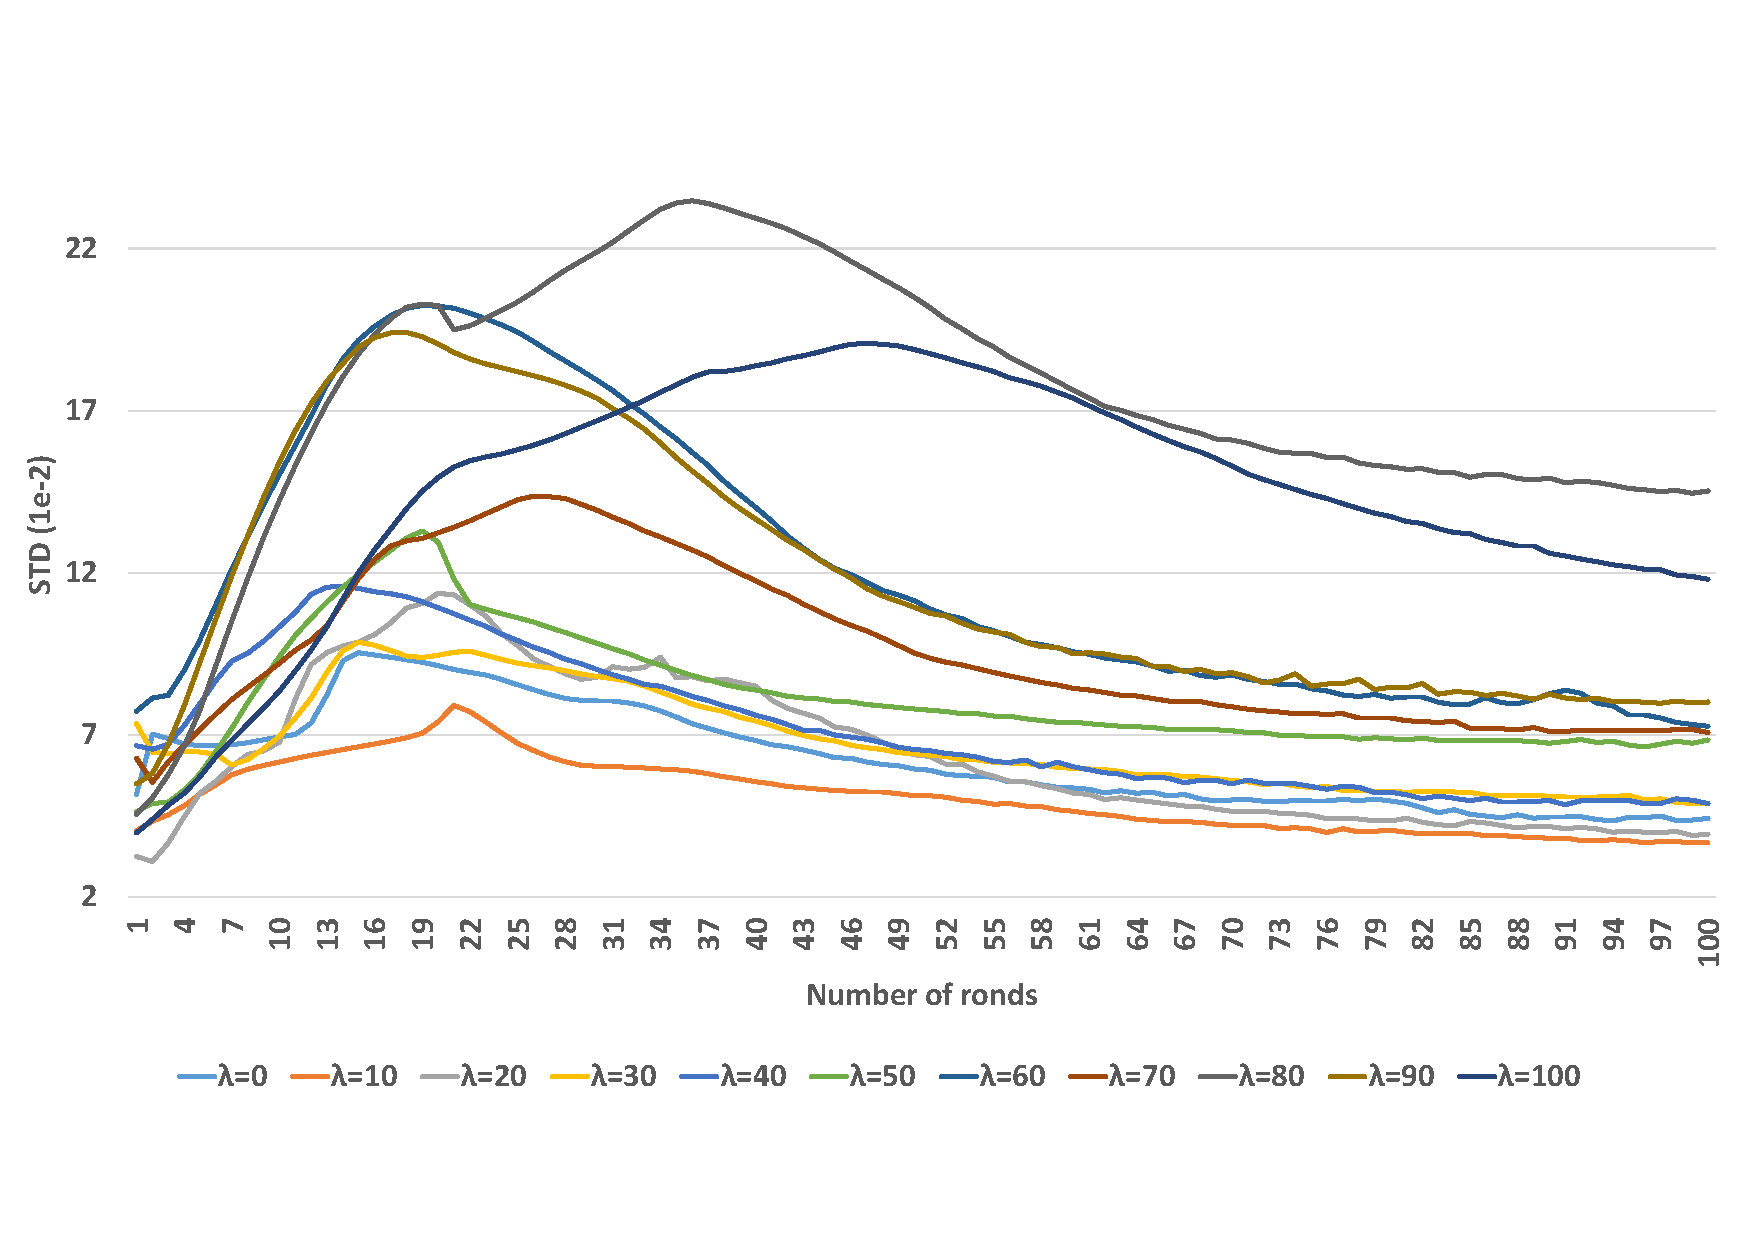
\includegraphics[scale=0.14]{./picture/select_function_unet_std_mean.pdf}}
	\caption{\textbf{Personalizing ratio and STD}. Sub-figure (a) and (b) shown personalizing ratio and classifier's parameters' mean STD between different clients in classification task and sub-figure (c) and (d) shown identical metric in segmentation task. In total, personalizing ratio increases with $\lambda$ becoming larger.}
	\label{fig_lambda_select_result}
\end{figure}

To study personalizing of classifier or decoder, we select $\lambda$ varying from 0 to 100 in Equation \ref{divergence_aggregate} with $\alpha=0$ in Equation \ref{whole_loss}. The results of classification task which are shown from sub-figure (a) to (d) and segmentation task which are shown from sub-figure (e) to (h) in Figure \ref{fig_luna_lambda_result}. 

In classification task, as label becoming unbalanced, higher BMACC requires larger $\lambda$ while BMBACC and BMCAF1 require relatively smaller $\lambda$. However in segmentation task, BMIoU and BMDice are almost no change when modal becomes unbalanced. From the result of these task in different data distribution, we concluded that personalizing should be related with proportion of category  instead of proportion of modals' composition. And slightly personalizing will get high BMACC in label unbalanced data.

\begin{figure}
	\centering
	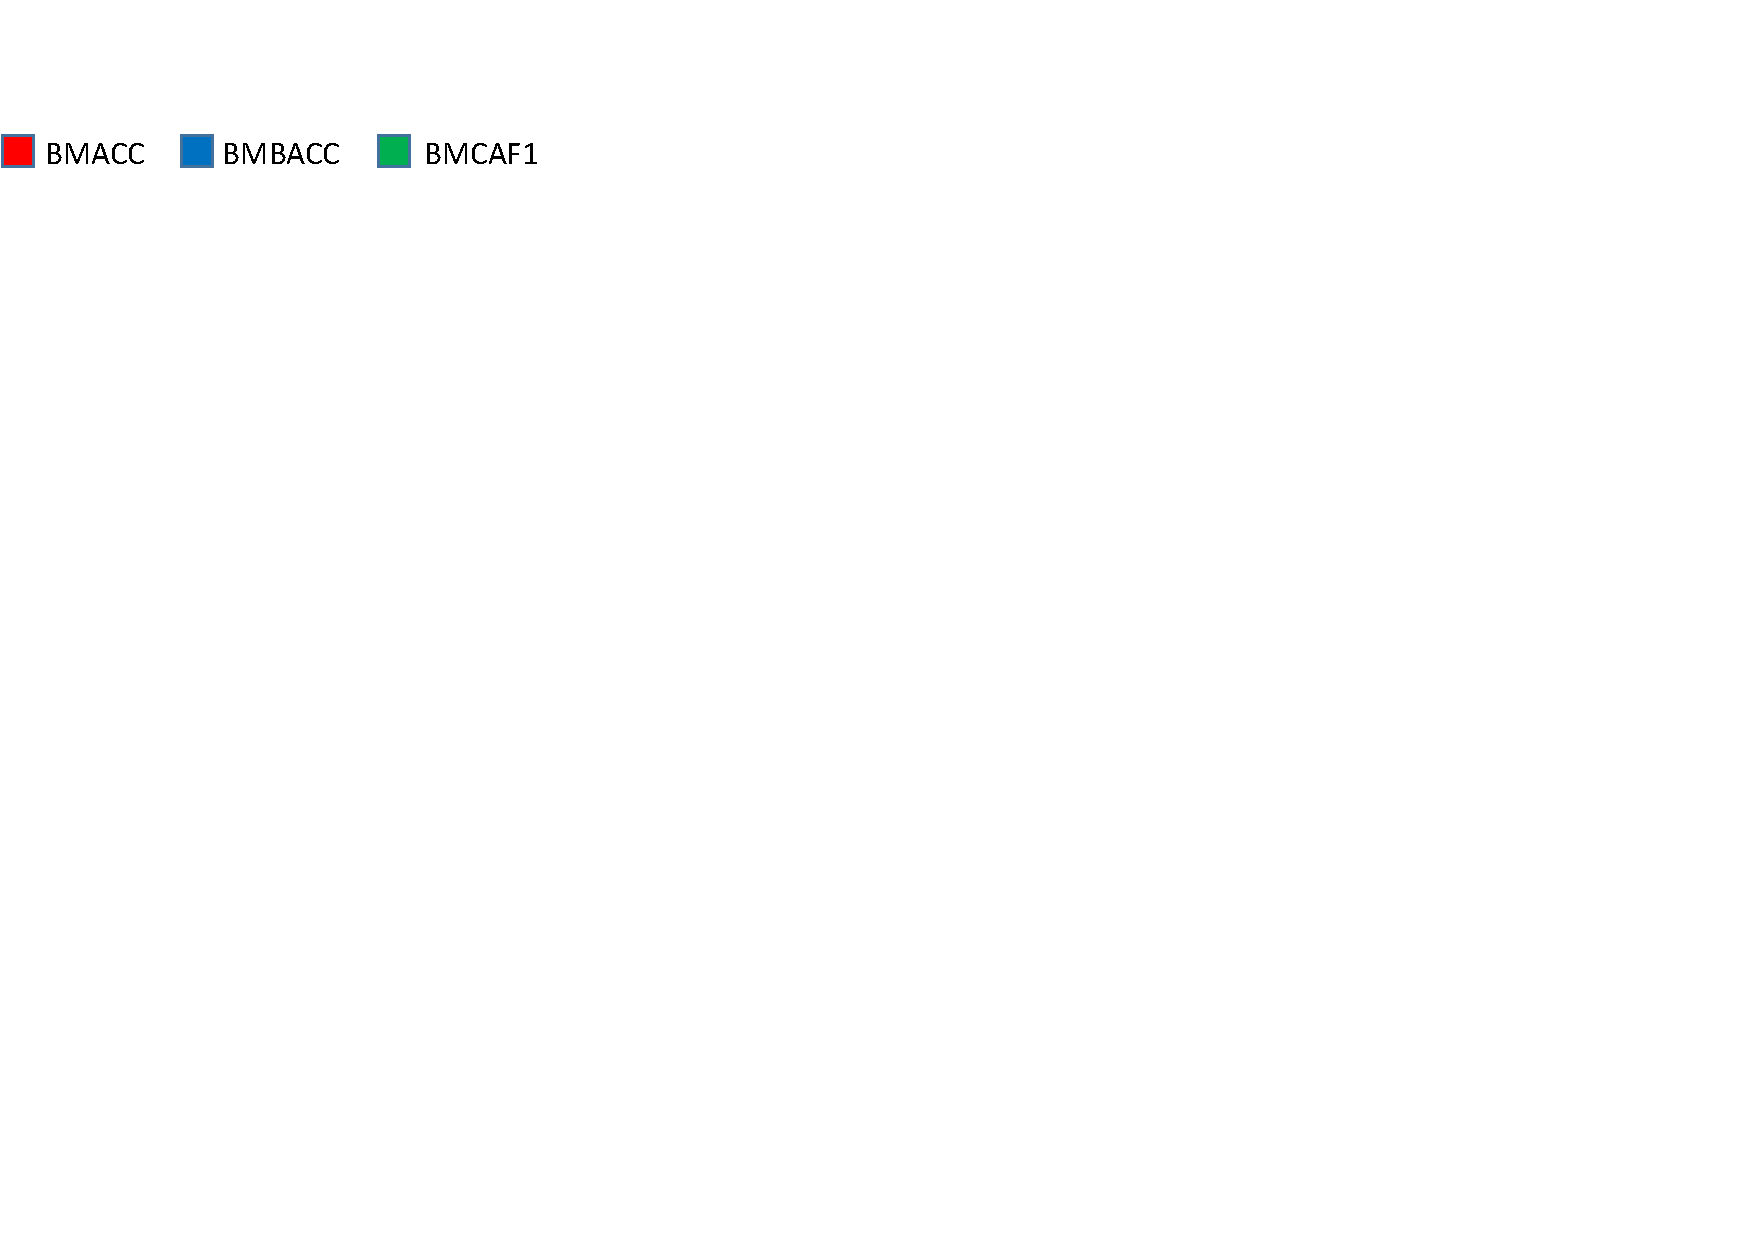
\includegraphics[scale=0.25,trim=0 550 0 0]{./picture/alpha_fig_ledgend.pdf}
	\subfigure[$\delta=1$]{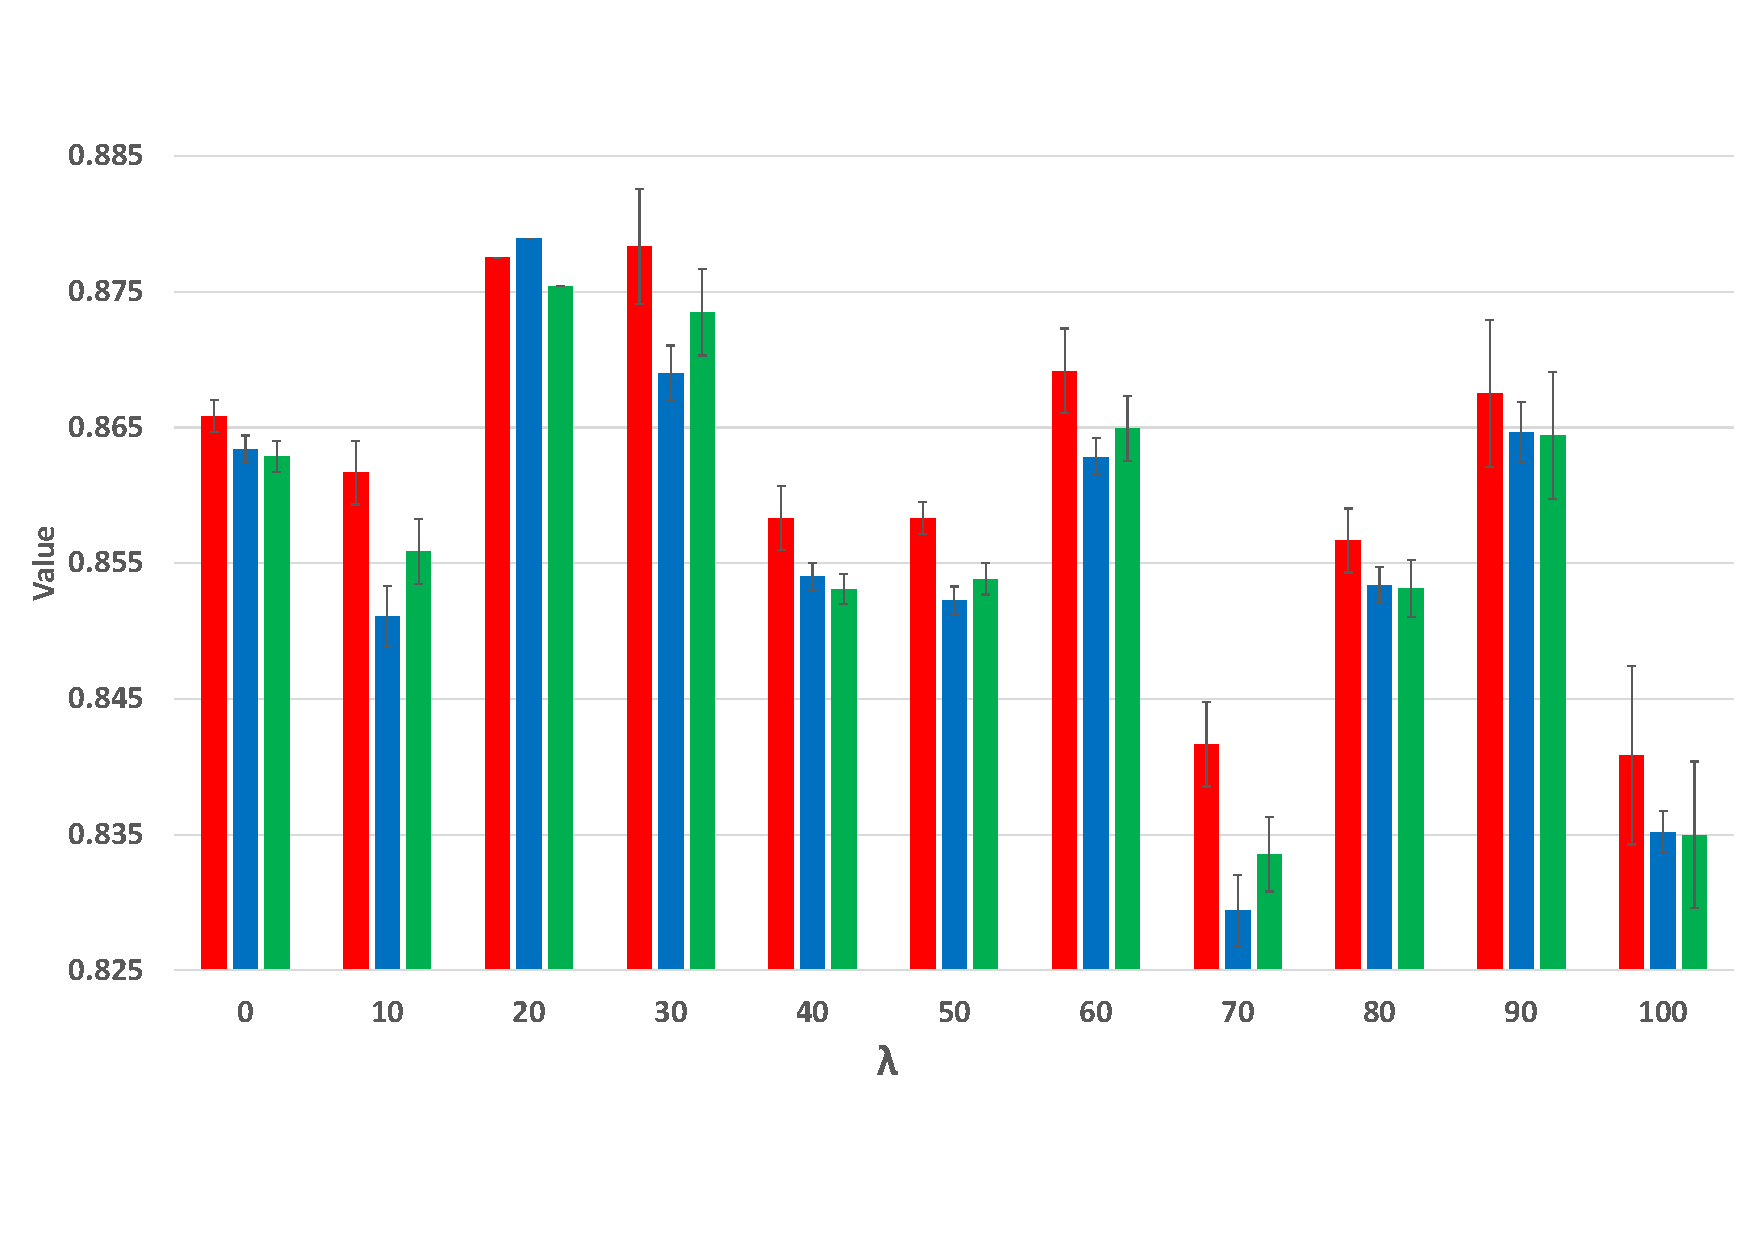
\includegraphics[scale=0.14]{./picture/delta1_lambda.pdf}}
	\subfigure[$\delta=2$]{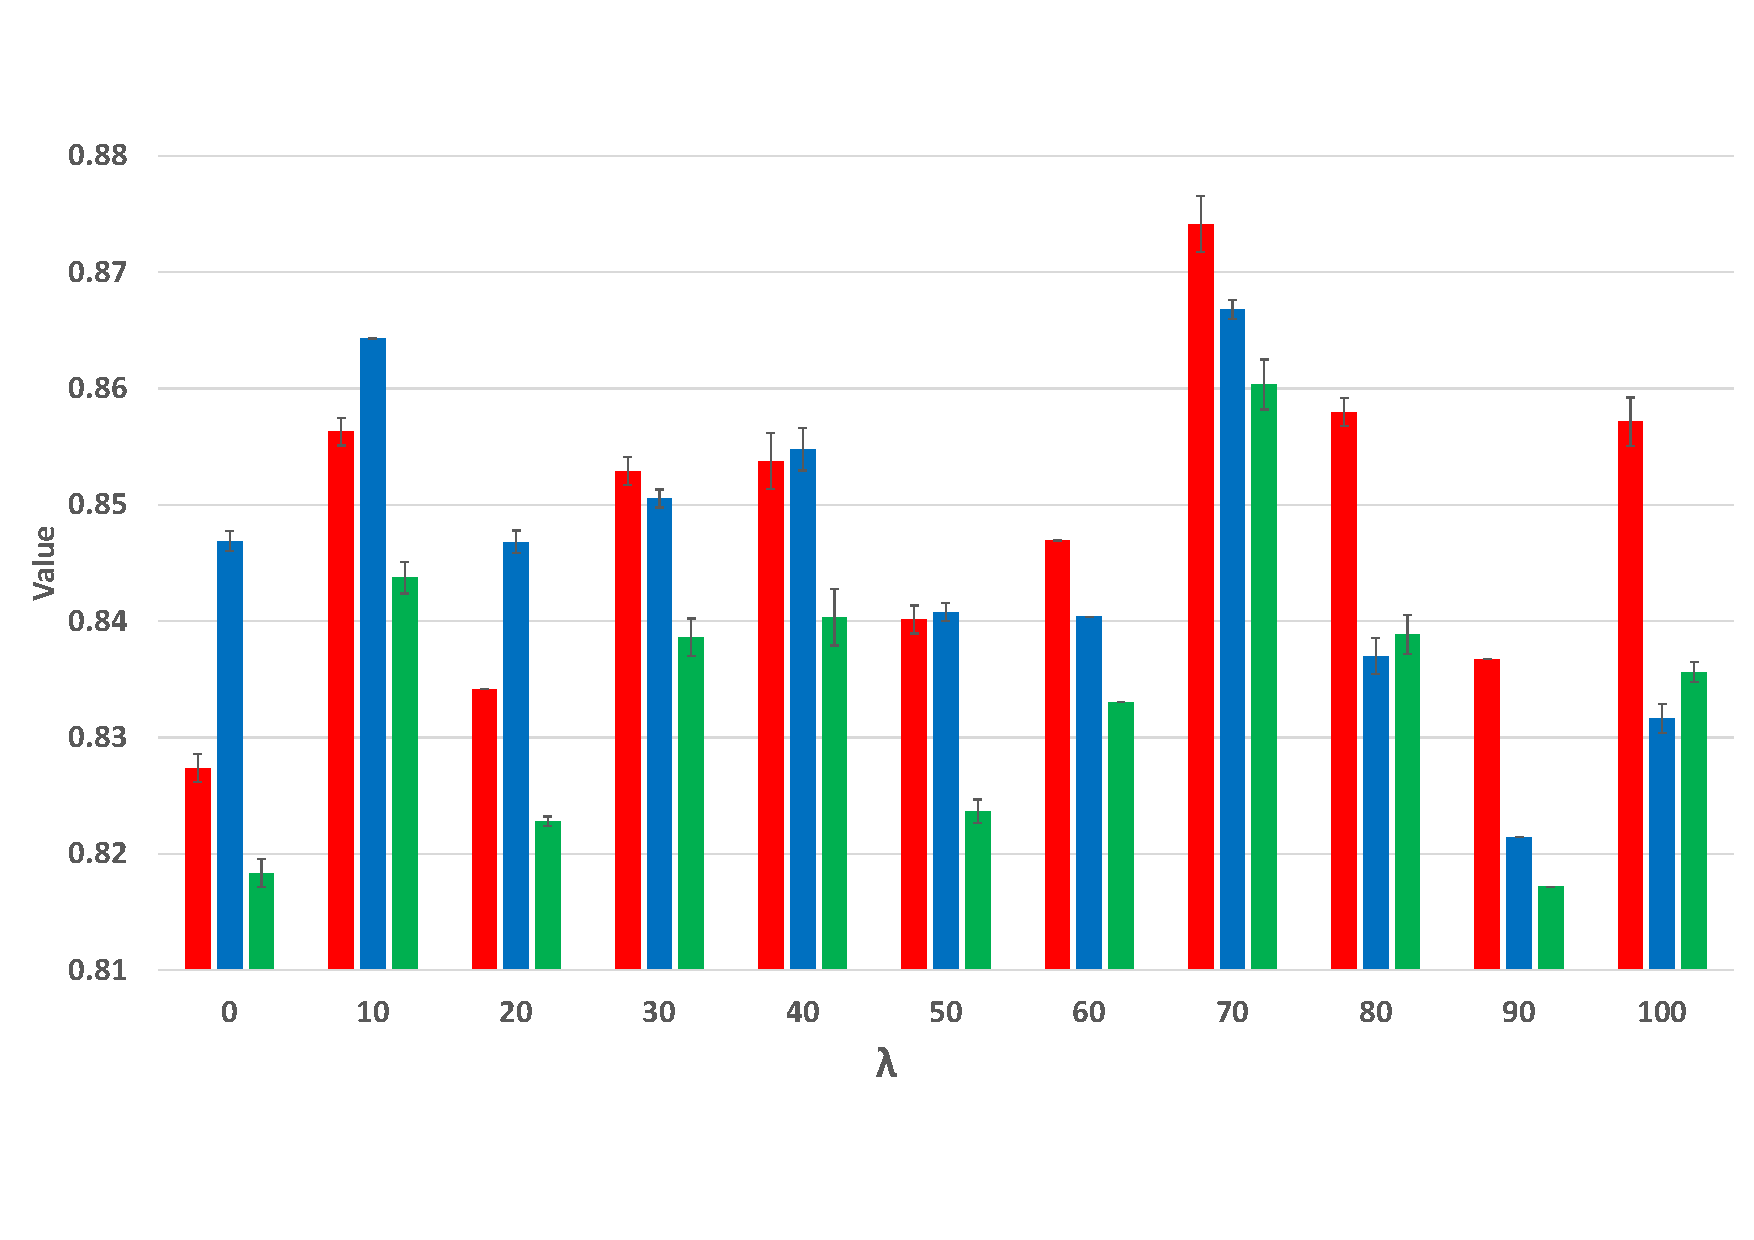
\includegraphics[scale=0.14]{./picture/delta2_lambda.pdf}}
	\subfigure[$\delta=4$]{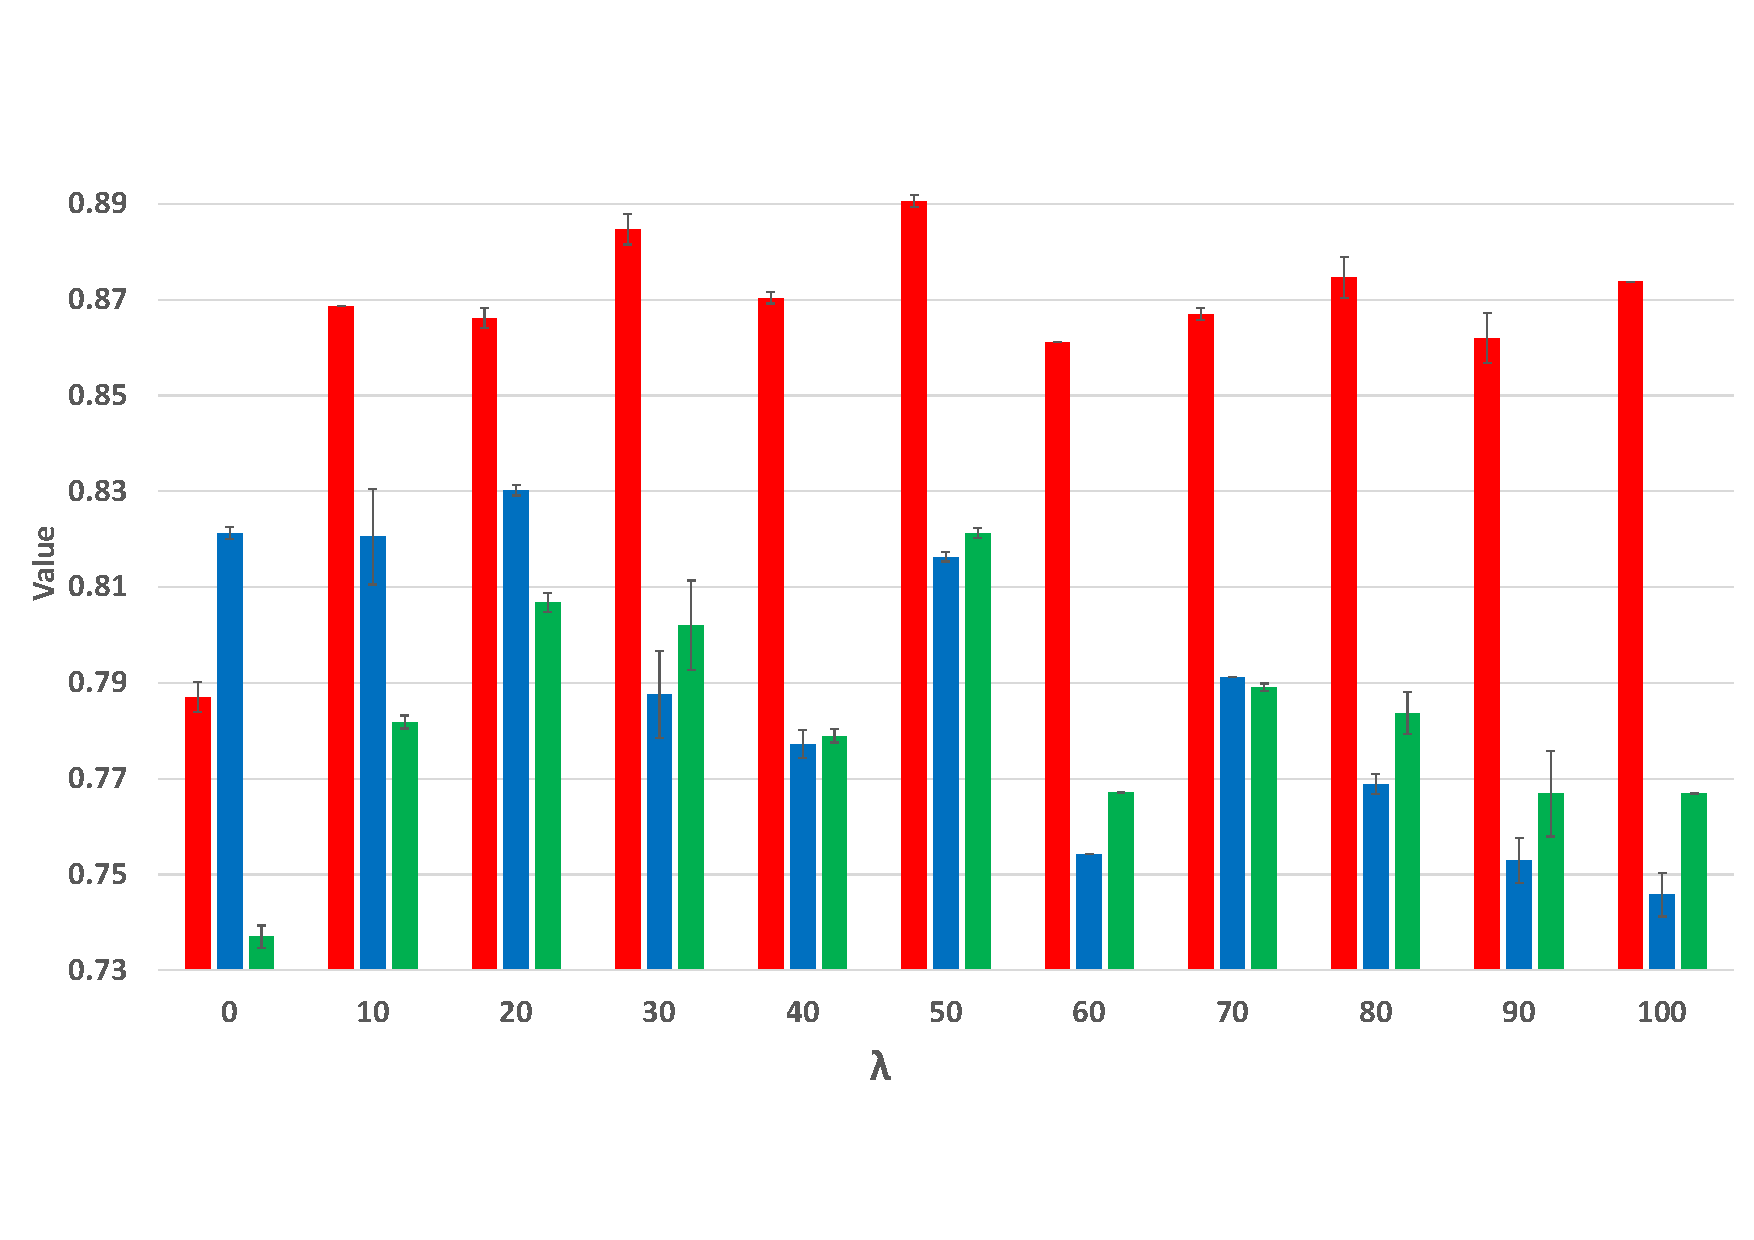
\includegraphics[scale=0.14]{./picture/delta4_lambda.pdf}}
	\subfigure[$\delta=7$]{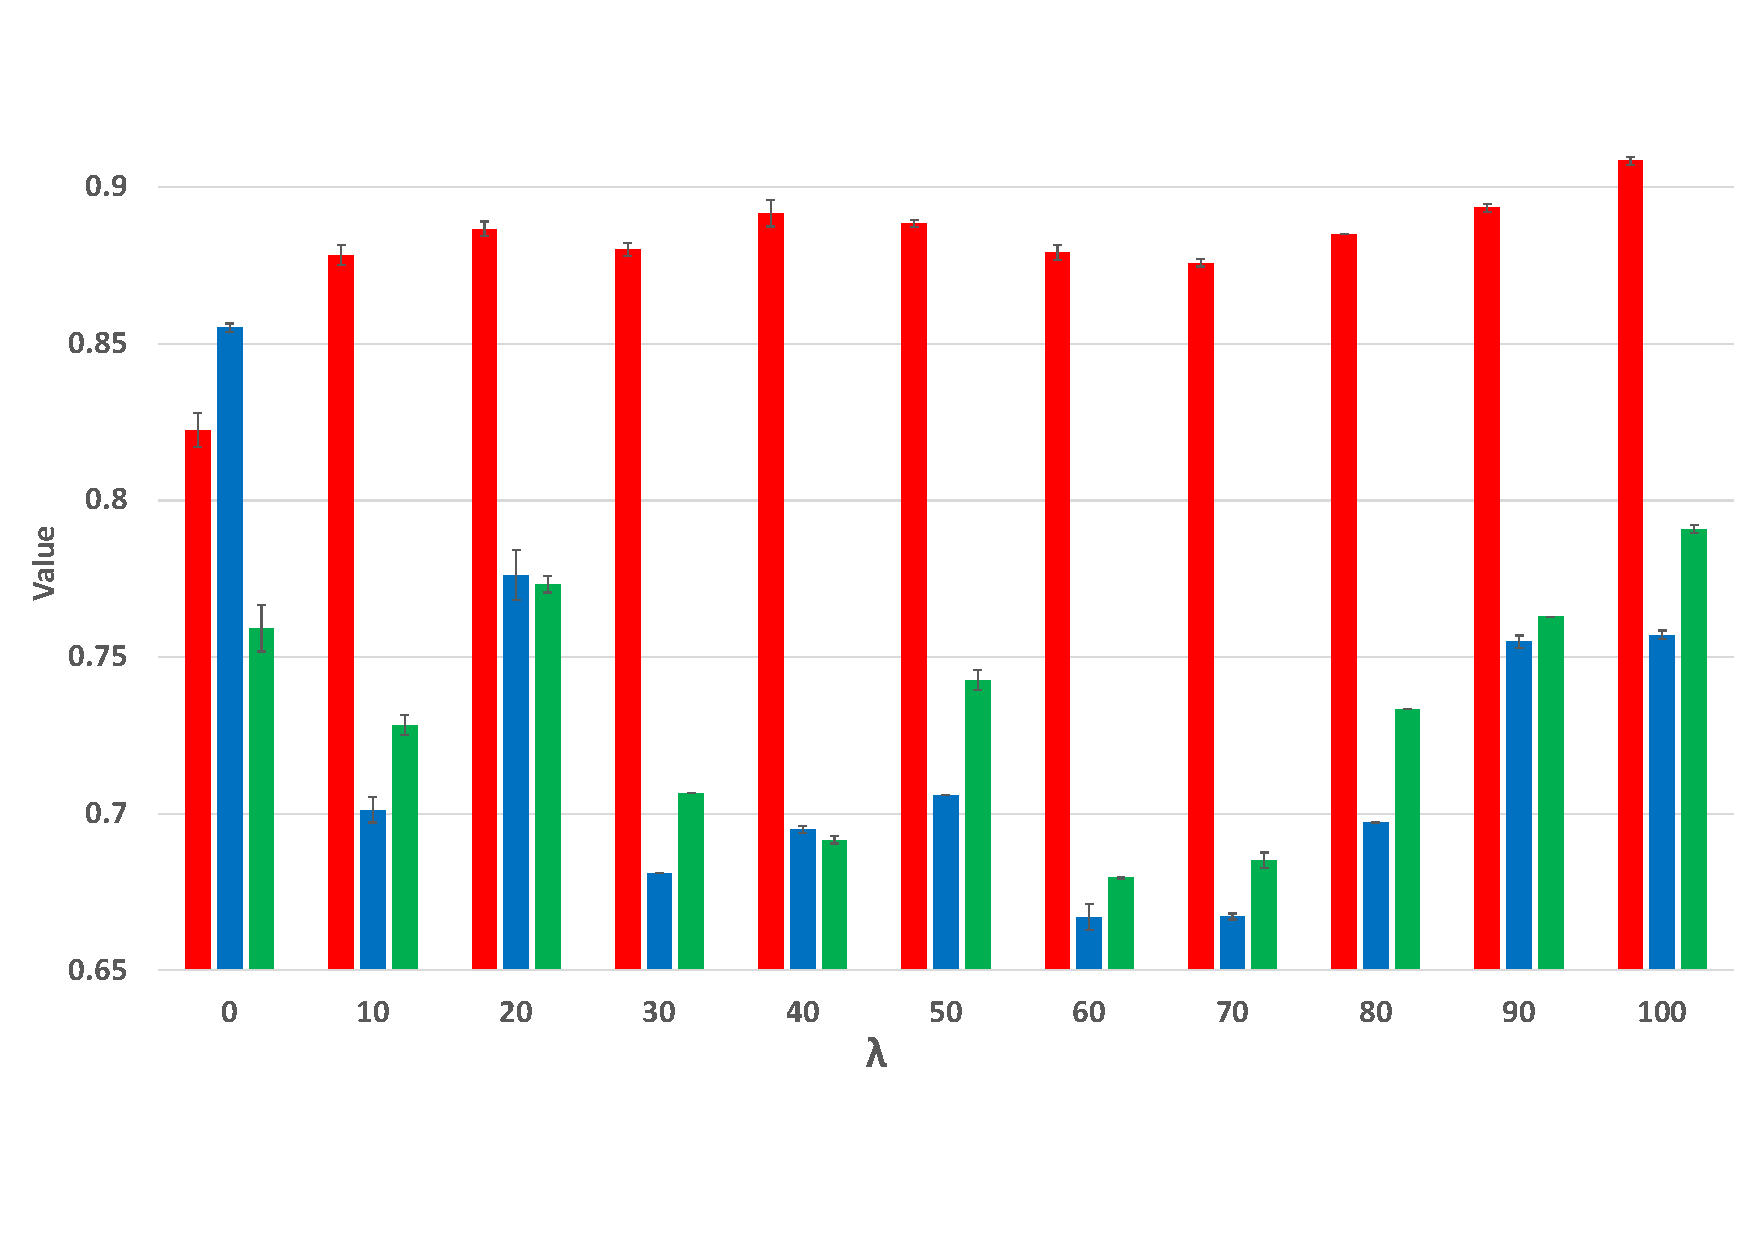
\includegraphics[scale=0.14]{./picture/delta7_lambda.pdf}}
	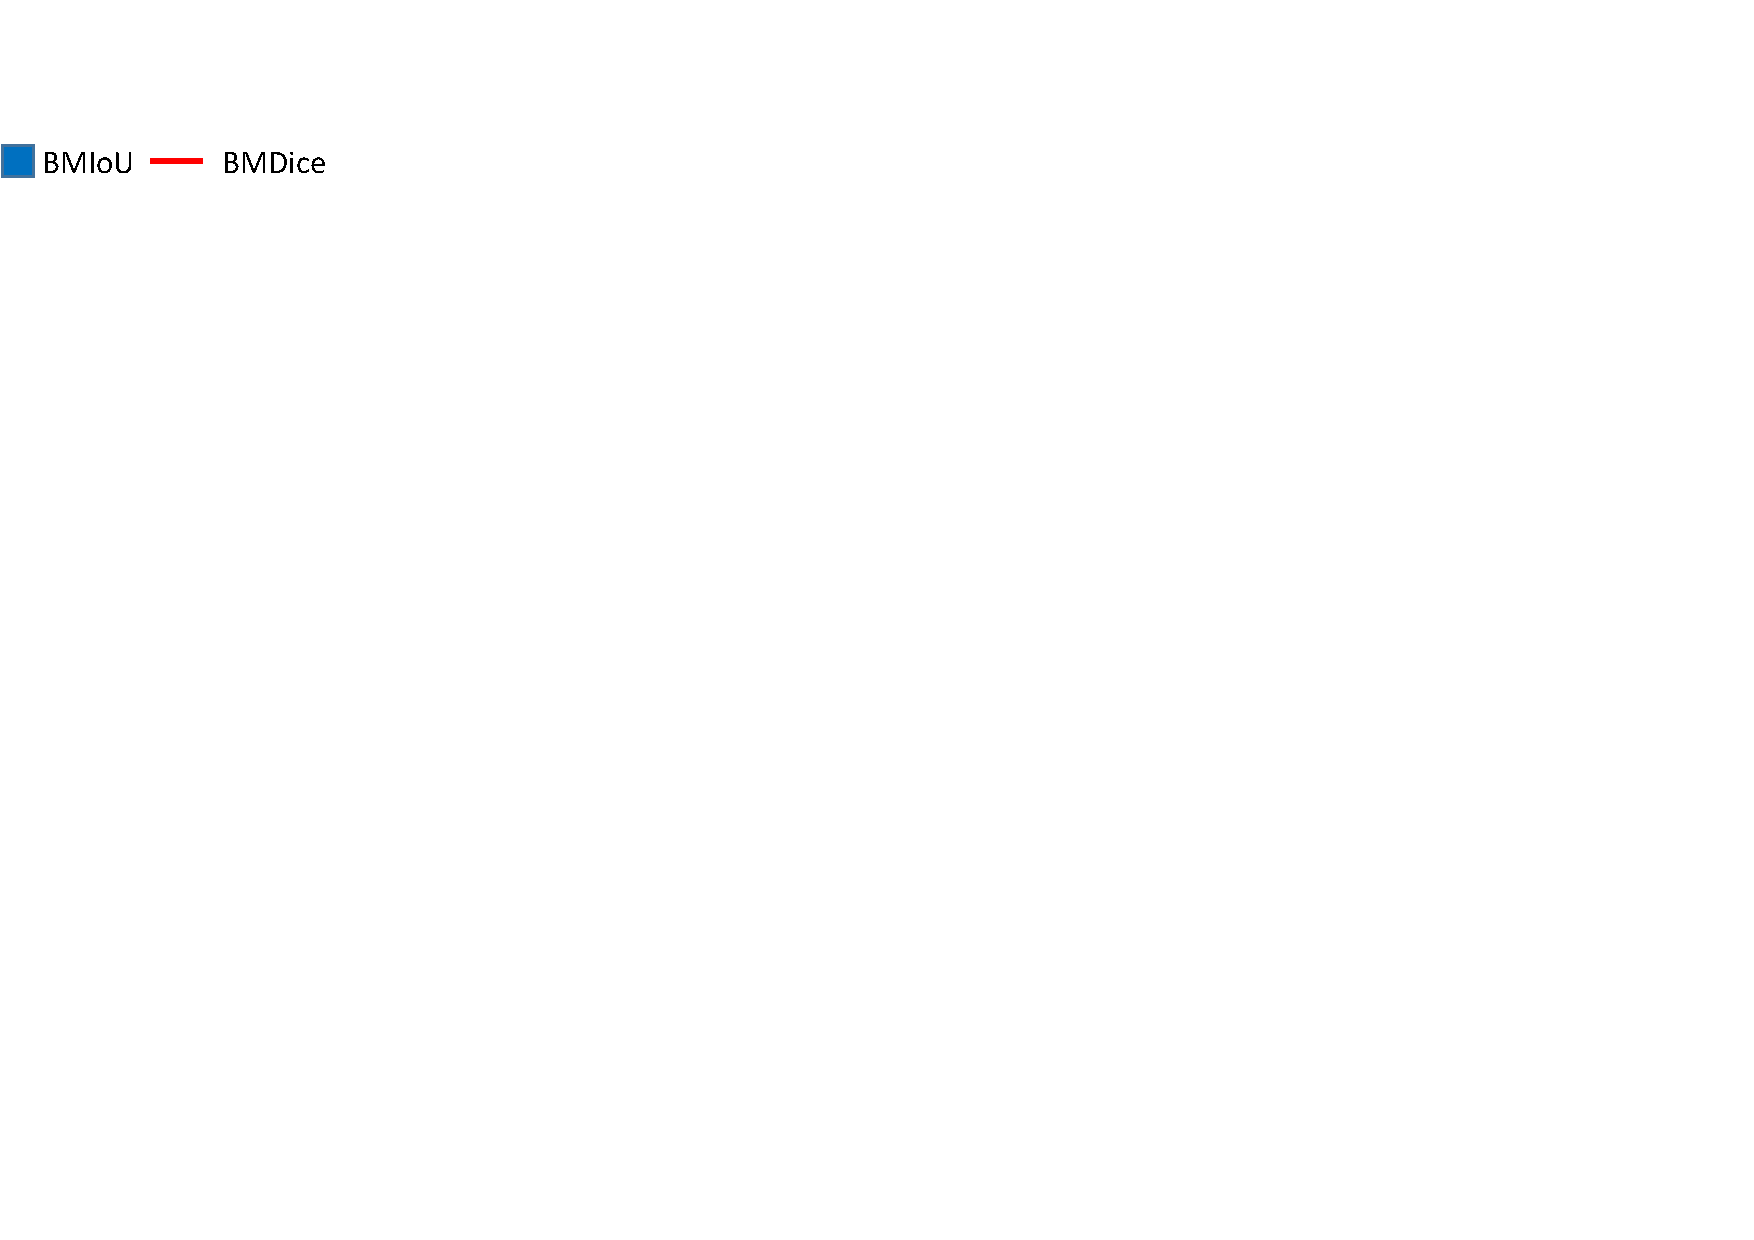
\includegraphics[scale=0.25,trim=0 550 0 0]{./picture/alpha_fig_unet_ledgend.pdf}
	\subfigure[$l=0$]{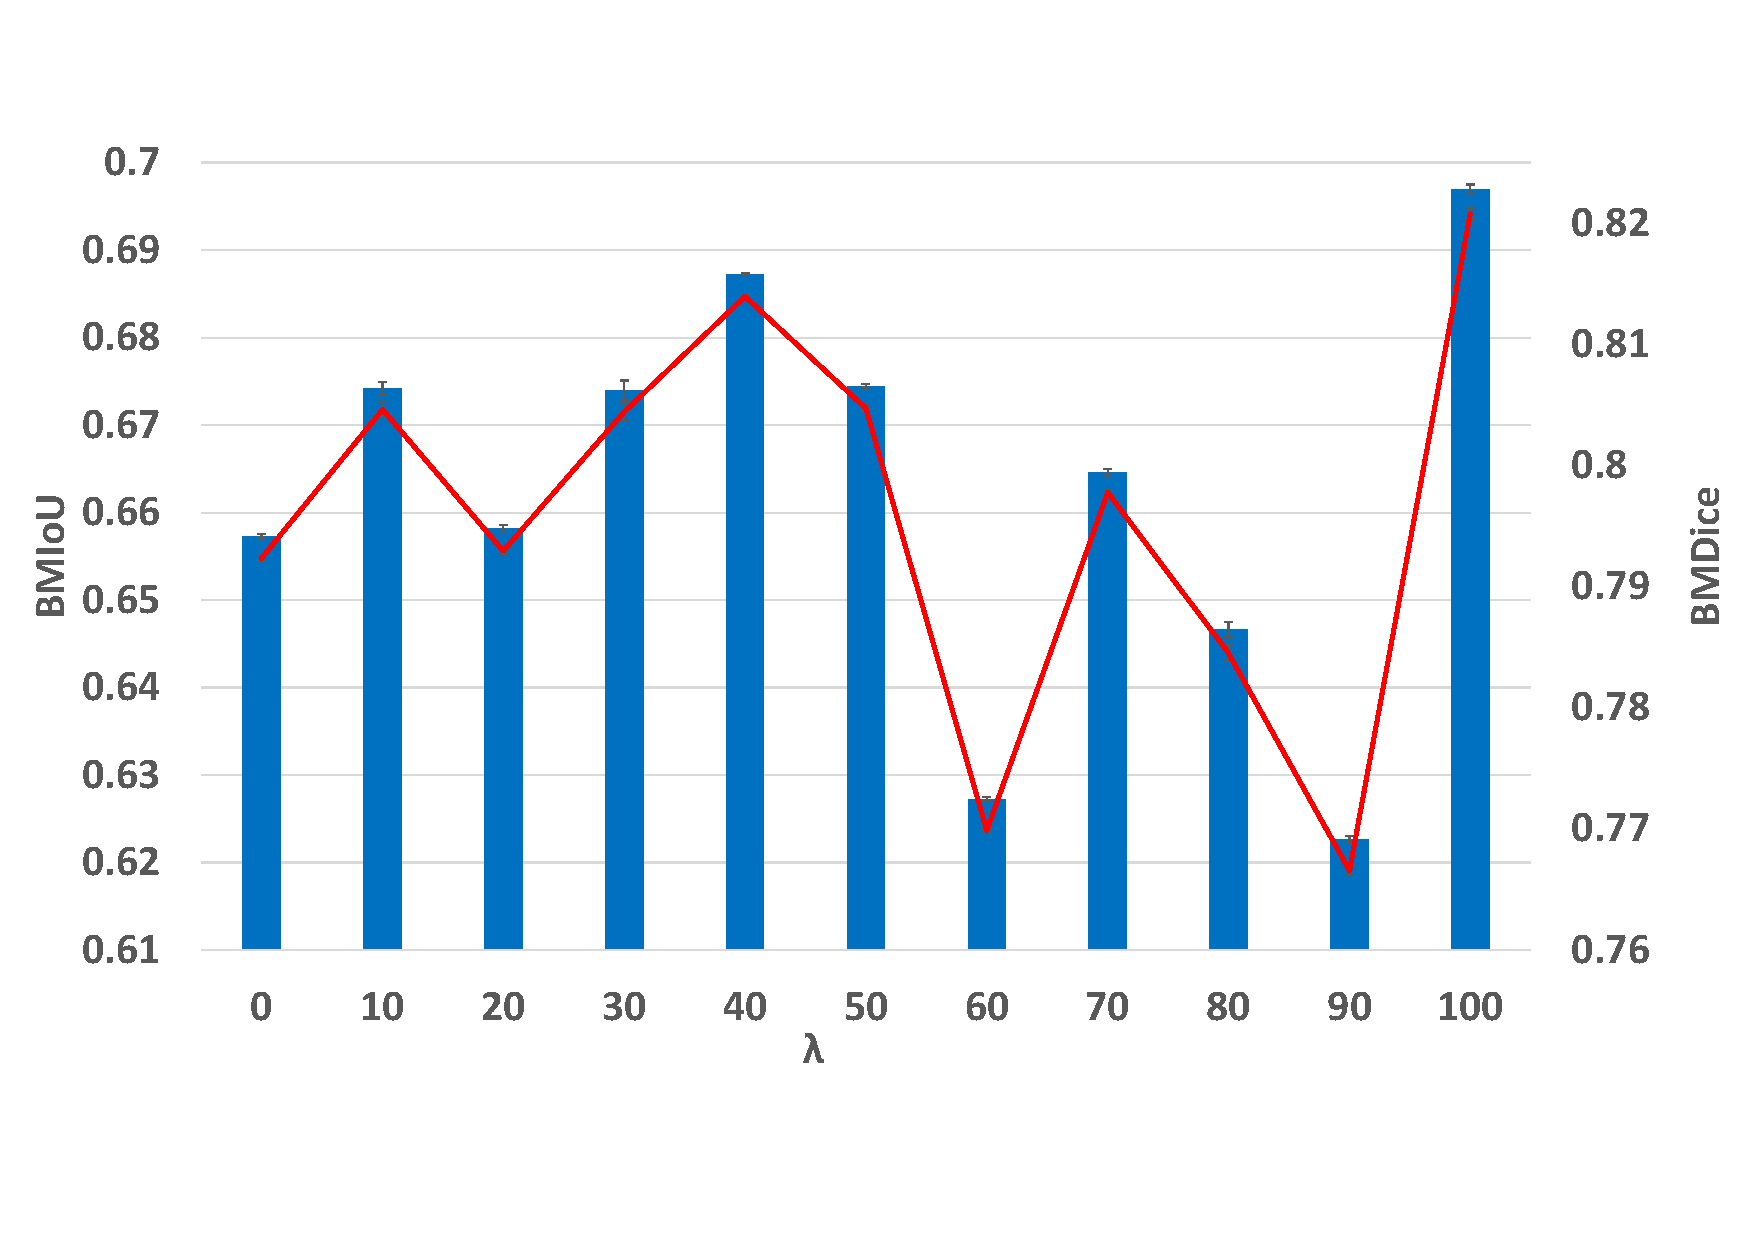
\includegraphics[scale=0.14]{./picture/lack0_lambda.pdf}}
	\subfigure[$l=1$]{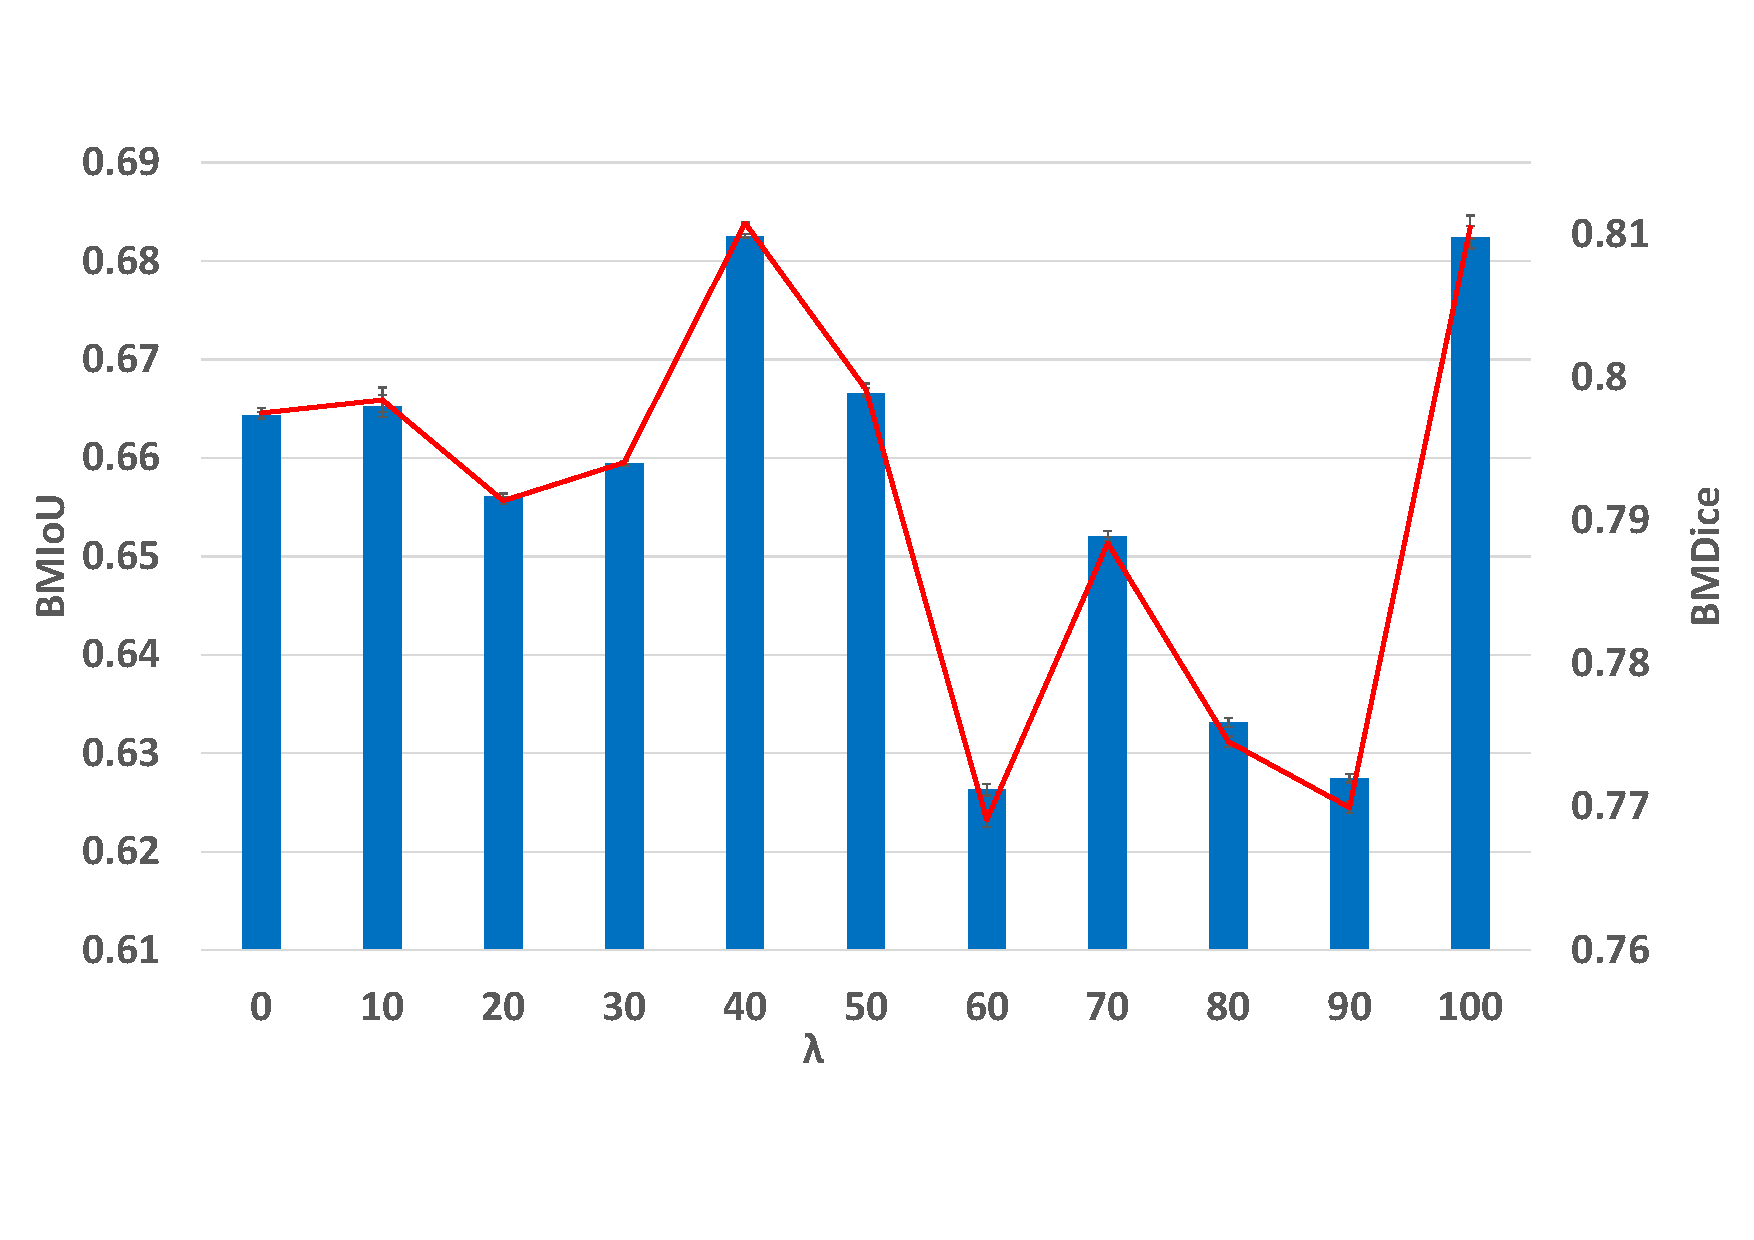
\includegraphics[scale=0.14]{./picture/lack1_lambda.pdf}}
	\subfigure[$l=2$]{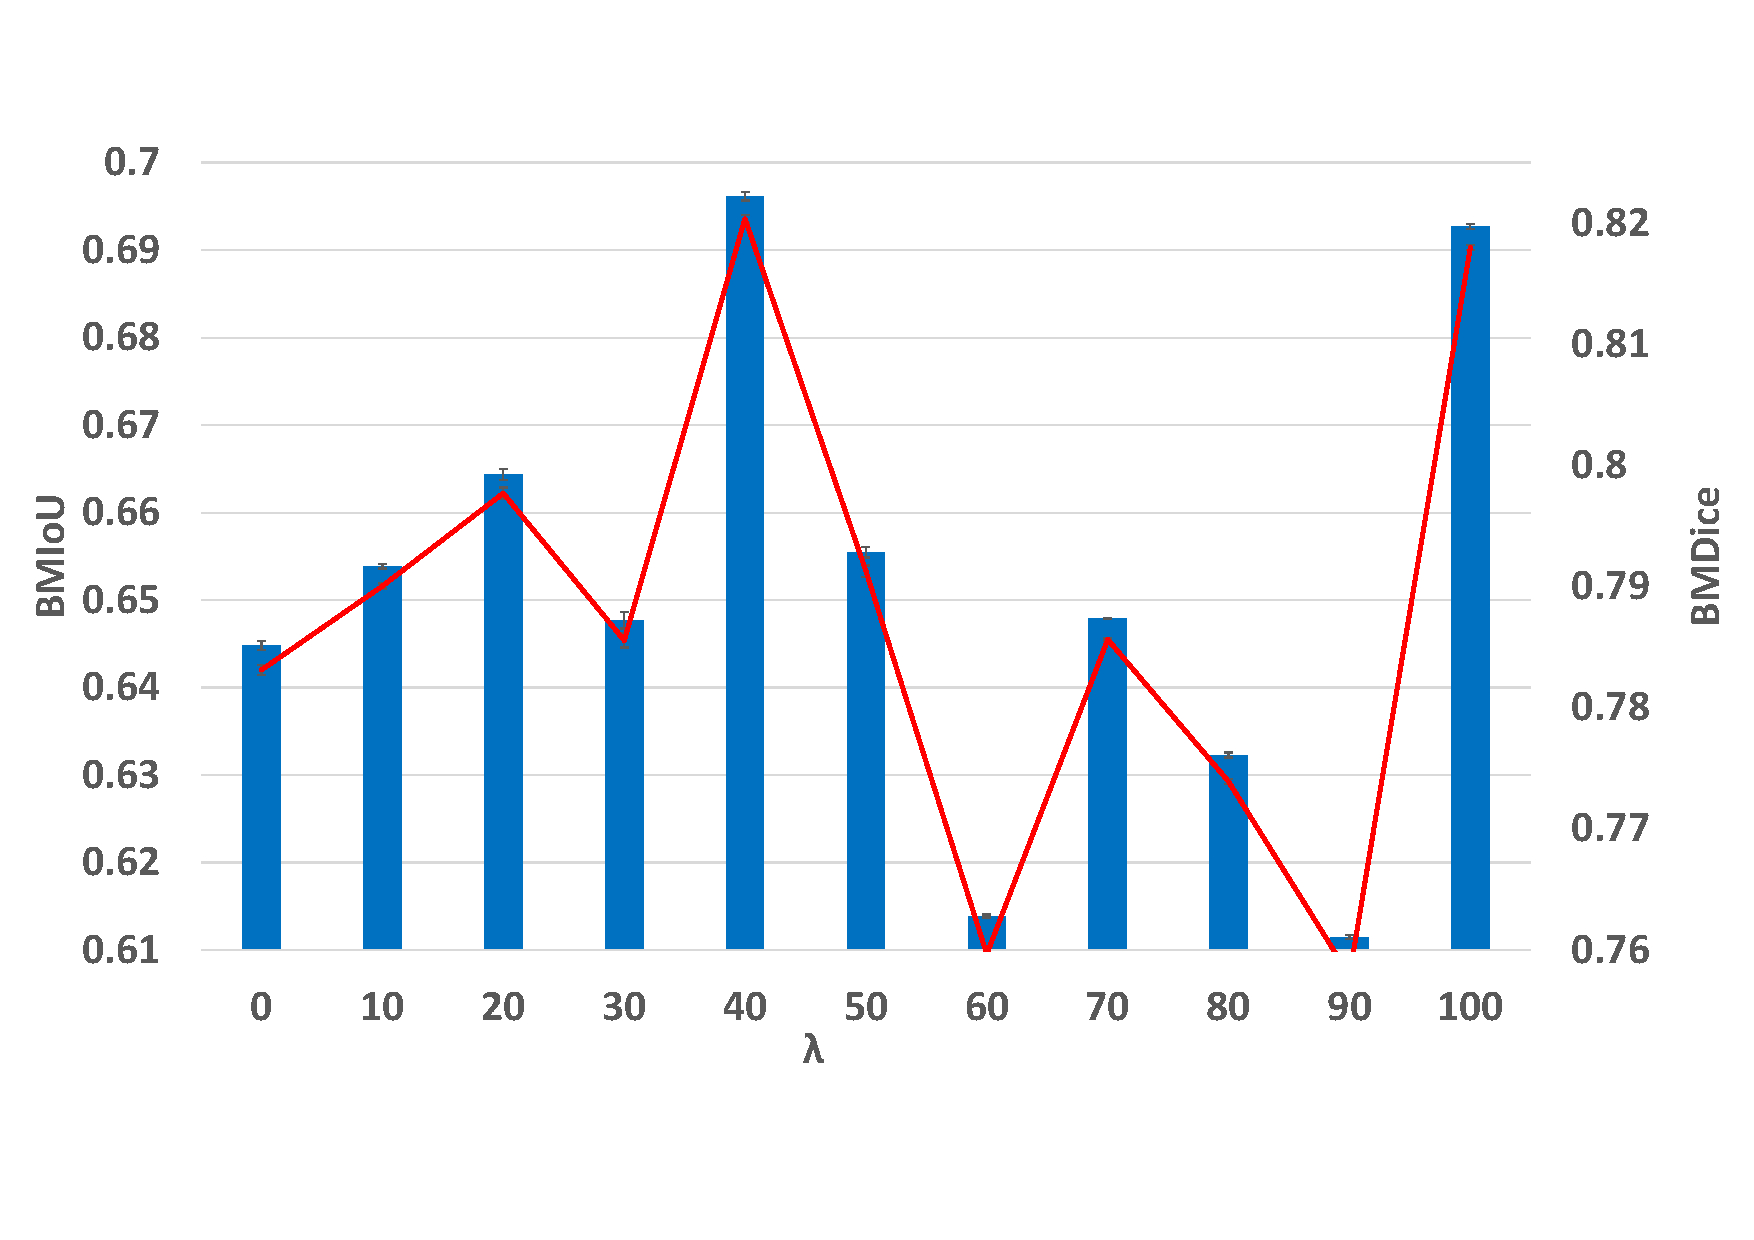
\includegraphics[scale=0.14]{./picture/lack2_lambda.pdf}}
	\subfigure[$l=3$]{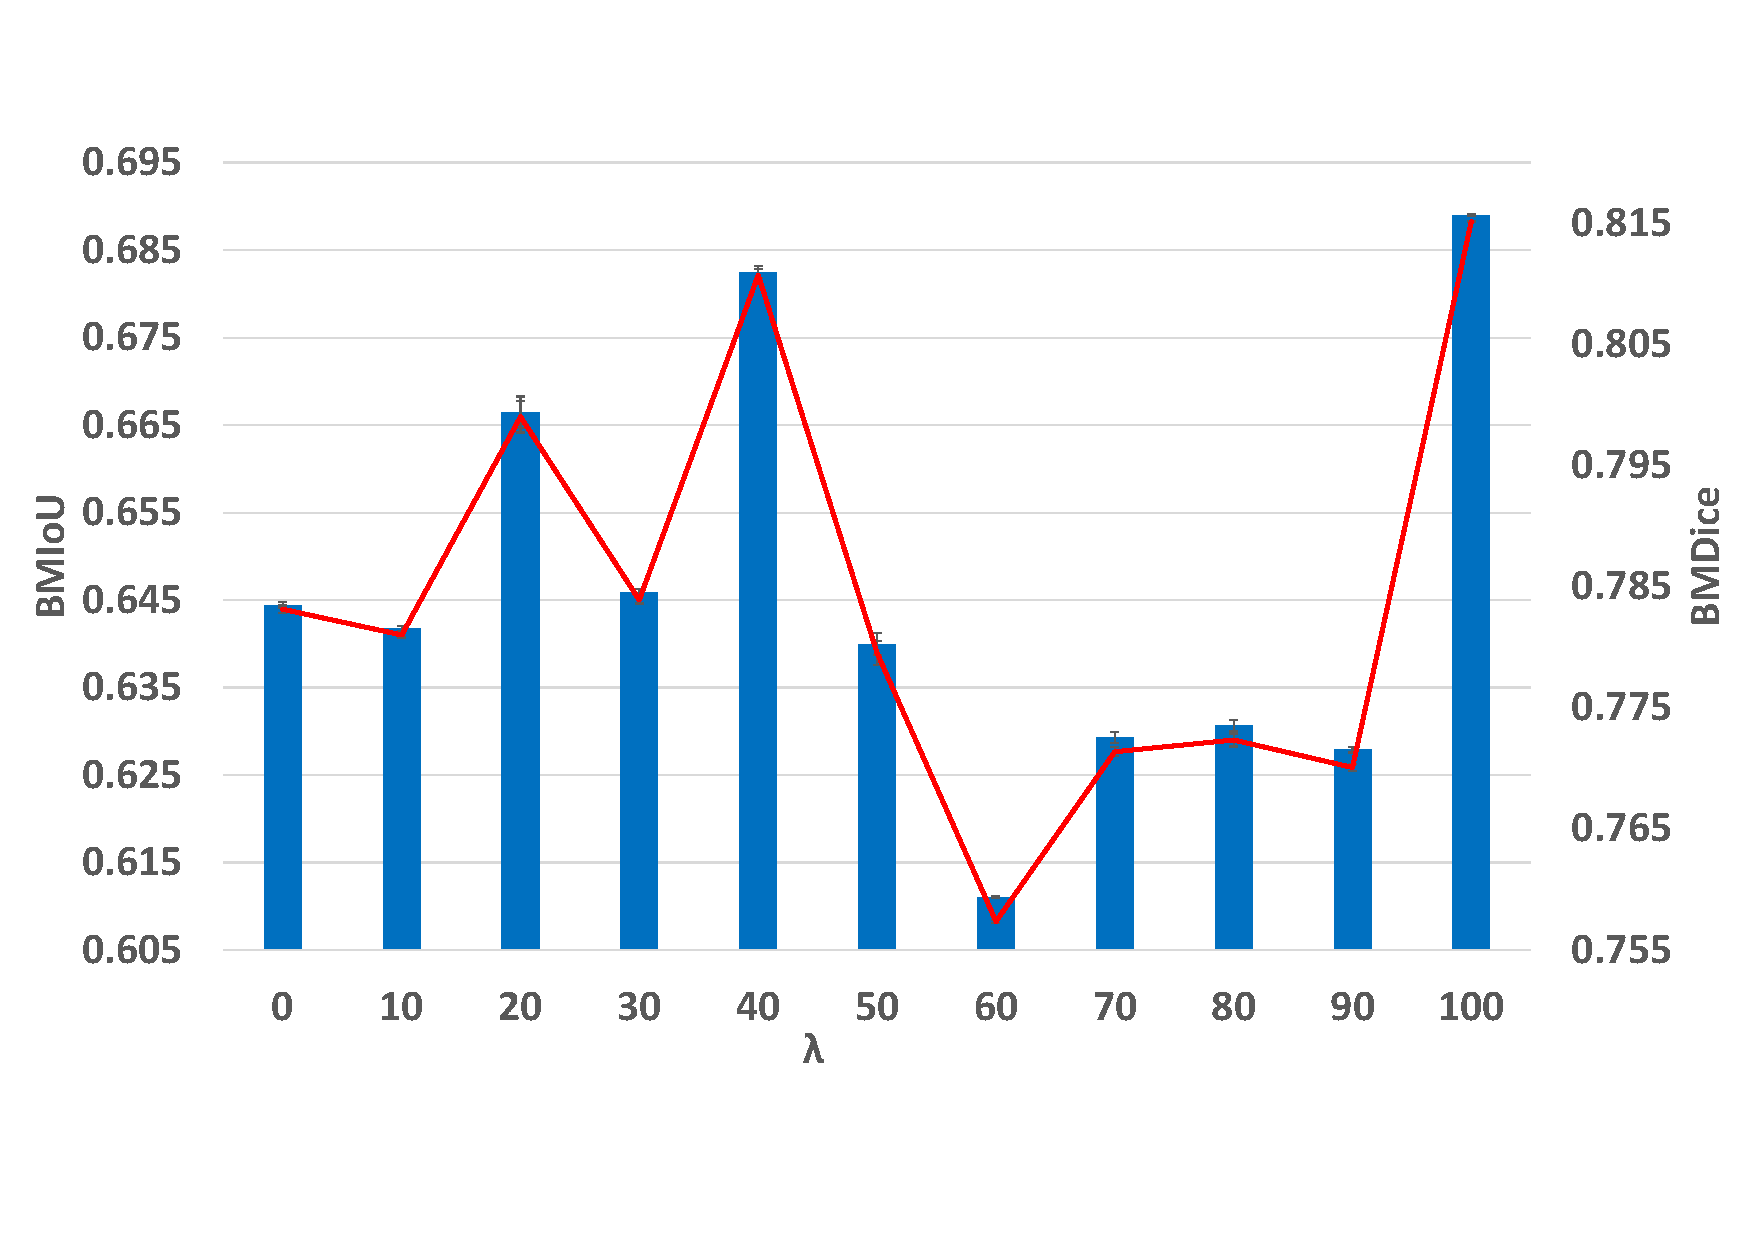
\includegraphics[scale=0.14]{./picture/lack3_lambda.pdf}}
	\caption{\textbf{Result on personalizing classifier or decoder}. The results of classification task which are shown from sub-figure (a) to (d) and segmentation task which are shown from sub-figure (e) to (h). Personalizing should be related with proportion of category instead of modals' composition}
	\label{fig_luna_lambda_result}
\end{figure}

\subsection{Compare with other strategies}
We compared 14 strategies include FedAvg, FedProx, FedAMP, FedRoD, L2GD, FPFC, IFCA, SuPerFed, Ditto, pFedME, FedPer, FedRep, pFedNet and FedABC to validate our strategy is superior performance in both classification task and segmentation task. We use BMACC, BMBACC and BMCAF1  in classification task and BMIoU, BMDice and BMSpec in segmentation task as the metric to compare strategies' performance. 

\subsubsection{Classification task}

We conducted classification task by LUNA16 with two label and DFUC 2021 with three label. These results are displayed in Table \ref{table_luna_classification} and Table \ref{table_dfuc_classification}. These tables shown our strategy's advantage over other strategies to some extent in both binary classification and multi classification task. 

In our compared strategies, FedRoD shows relative excellent performance for BMACC especially in the unbalanced data. The reason we guess is that FedRoD focus on the advantage data. Interms of BMACC, when the data distribution is extremely unbalanced the profit of correctly classifying advantaged category surpass the loss of mistakenly classifying disadvantaged category. Thus, the shortcoming of FedRod is that it's performance for BMBACC and BMCAF1 which pay more attention to disadvantaged category relative poor. While in medical industry minor group do important to diagnosis such as rare disease. 

Meanwhile, we couldn't ignore major popular otherwise high misdiagnose rate will impact hospitals' quality of health care. Thus, FedAvg, pFedNet and IFCA may not suitable strategies to screen in medicine though they have relative high BMBACC and BMCAF1. In other hand, IFCA needs repeatedly communicating between clients and server that will consume higher costs.

Our aggregation algorithm not only improves models performance in BMACC which majorly used in daily screening but also in BMBACC and BMCAF1 which majorly used in making a definite diagnosis. And it working well in different data distribute of binary or multi classification in terms of medical data.

\subsubsection{Segmentation task}
Some algorithms are not considering segmentation task. But in theory they can be used to that through deforming to some extent. We handled BraTS 2017 datasets as two targets and four targets in segmentation task. 

To build non-IID data, we treat the datasets' four channels as four views. It is hided to clients in different extent and we use $l$ denoting the this extent. If $l=n$, there are $n$ kind of view being hided to clients that views vary from clients. We called that as modal unbalanced. And these results are shown by Table \ref{table_Tram2_classification} and Table \ref{table_Tram4_classification}.

In two targets segmentation task, FedAvg, FedRoD and IFCA get relative considerable BMIoU and BMDice regardless of modal unbalanced. We guess that the volume in space of two targets is equal in expectation. When it comes to four targets segmentation, their BMIoU and BMDice are relative low. We assume that it was caused by their overlook about minorities. 

FedAMP and L2GD achieved relatively high BMIoU and BMDice in extremely modal unbalanced data in four targets segmentation task. But their methods to aggregate models' weight would cost higher calculate resource especially when the quantity of clients is large. And their performance in other distribution are not well. We think that their gradient directions are lead by all clients and it is easily mislead by some outliers.

Segmentation task in medical diagnosis is relative unimportant, but they absolutely play significant role in surgery. If the machine's sensitive is not enough, the health organize may be resected wrongly which is intolerable in brain surgery. While cancer will be remained in body which maybe fatal when machine's specificity is low. And our strategy not only considers sensitive but also specificity which has higher accuracy comparing to other strategies.

\section{Conclusion}
In this paper, we consider the medical actual scenery and compare different strategies in special metrics which are more accepted by medicine. Thinking about that there different kind of data distribution in real works, we built different types of distribution data including label unbalanced and modal unbalance. And we validated that our strategy is relative advance over others we compared in different scene. But supervised learning may not suite large scale federated learning, we will pay more attention to semi-supervised or unsupervised learning base on this work in the future.

\bibliographystyle{IEEEtran}  
\bibliography{reference}


\onecolumn
\begin{table}
	\caption{Results of binary label classification task\\
		on LUNA16} 
	\label{table_luna_classification}
	\centering
	\begin{subtable}[]{$\delta=1$}
		\begin{tabular}{lccc}
			%& \multicolumn{3}{c}{delta=1}    
			\toprule  
			\specialrule{0em}{3pt}{1pt}                                          
			& BMACC                  & BMBACC                  & BMCAF1                  \\ \midrule
			FedAvg   & 87.00$\pm$0.00         & 85.78$\pm$0.00          & 86.39$\pm$0.00          \\
			FedProx  & 82.92$\pm$0.24         & 81.11$\pm$0.04          & 81.68$\pm$0.06          \\
			Ditto    & 84.50$\pm$0.00         & 83.56$\pm$0.09          & 83.78$\pm$0.07          \\
			FedPer   & 77.08$\pm$0.62         & 77.05$\pm$0.21          & 76.68$\pm$0.40          \\
			FedRep   & 82.67$\pm$0.72         & 82.34$\pm$0.57          & 82.25$\pm$0.69          \\
			FedRoD   & 87.00$\pm$0.00         & 86.40$\pm$0.06          & 86.56$\pm$0.04          \\
			FPFC     & 76.25$\pm$0.00         & 73.96$\pm$0.13          & 74.41$\pm$0.11          \\
			IFCA     & 85.08$\pm$0.12         & 83.93$\pm$0.12          & 84.44$\pm$0.12          \\
			pFedME   & 79.58$\pm$0.31         & 77.90$\pm$0.20          & 78.35$\pm$0.24          \\
			SuperFed & 69.92$\pm$1.30         & 70.25$\pm$0.72          & 68.61$\pm$1.11          \\
			FedAMP   & 79.33$\pm$0.31         & 78.17$\pm$0.27          & 78.44$\pm$0.30          \\
			L2GD   & 77.00$\pm$0.20         & 75.65$\pm$0.07          & 75.94$\pm$0.09          \\
			pFedNet  & 85.50$\pm$0.00         & 85.40$\pm$0.00          & 85.25$\pm$0.00          \\
			FedABC   & 71.00$\pm$0.00         & 71.61$\pm$0.10          & 70.83$\pm$0.02          \\
			%\midrule
			FedDiv   & \textbf{88.5$\pm$0.20} & \textbf{88.18$\pm$0.14} & \textbf{88.19$\pm$0.19} \\
			\bottomrule
		\end{tabular}
	\end{subtable}
	\centering
	\begin{subtable}[]{$\delta=2$}
		\begin{tabular}{lccc}
			\toprule  
			\specialrule{0em}{3pt}{1pt}  
			& BMACC                  & BMBACC                  & BMCAF1                  \\ \midrule
			FedAvg   & 83.93$\pm$0.21          & 84.49$\pm$0.22          & 82.66$\pm$0.20          \\
			FedProx  & 79.76$\pm$0.12          & 80.49$\pm$0.33          & 78.31$\pm$0.12          \\
			Ditto    & 80.87$\pm$0.42          & 81.45$\pm$0.49          & 79.16$\pm$0.33          \\
			FedPer   & 79.51$\pm$0.12          & 73.19$\pm$0.83          & 74.53$\pm$0.81          \\
			FedRep   & 83.50$\pm$0.12          & 78.97$\pm$0.42          & 80.21$\pm$0.27          \\
			FedRoD   & 86.39$\pm$0.12          & 84.69$\pm$0.04          & 84.49$\pm$0.11          \\
			FPFC     & 76.45$\pm$0.43          & 73.79$\pm$0.26          & 73.23$\pm$0.32          \\
			IFCA     & 84.95$\pm$0.21          & 85.25$\pm$0.22          & 83.65$\pm$0.22          \\
			pFedME   & 78.15$\pm$0.12          & 77.51$\pm$0.45          & 75.89$\pm$0.43          \\
			SuperFed & 75.94$\pm$0.64          & 71.22$\pm$0.73          & 70.95$\pm$1.13          \\
			FedAMP   & 72.28$\pm$0.12          & 74.29$\pm$0.67          & 73.20$\pm$0.21          \\
			L2GD   & 76.70$\pm$0.60          & 73.84$\pm$0.20          & 73.19$\pm$0.65          \\
			pFedNet  & 82.40$\pm$0.00          & 84.55$\pm$0.05          & 81.48$\pm$0.02          \\
			FedABC   & 76.79$\pm$0.21          & 72.31$\pm$0.22          & 70.22$\pm$0.21          \\ %\midrule
			FedDiv   & \textbf{86.99$\pm$0.00} & \textbf{85.40$\pm$0.00} & \textbf{85.30$\pm$0.00} \\ 
			\bottomrule 
		\end{tabular}
	\end{subtable}
	\centering
	\\
	\begin{subtable}[]{$\delta=4$}
		\begin{tabular}{lccc}
			\specialrule{0em}{3pt}{1pt}
			\toprule
			FedAvg   & 84.76$\pm$0.31          & 84.99$\pm$0.30          & 79.80$\pm$0.57          \\
			FedProx  & 82.66$\pm$0.66          & 84.12$\pm$0.65          & 77.77$\pm$0.57          \\
			Ditto    & 86.20$\pm$0.83          & 81.27$\pm$1.13          & 77.18$\pm$0.48          \\
			FedPer   & 83.84$\pm$0.41          & 62.11$\pm$1.02          & 62.96$\pm$1.22          \\
			FedRep   & 86.78$\pm$0.43          & 69.92$\pm$1.04          & 73.24$\pm$1.43          \\
			FedRoD   & \textbf{91.75$\pm$0.31} & 84.28$\pm$0.81          & 86.26$\pm$0.28          \\
			FPFC     & 82.66$\pm$0.12          & 71.65$\pm$0.17          & 72.19$\pm$0.17          \\
			IFCA     & 88.72$\pm$0.12          & 86.93$\pm$0.07          & 83.59$\pm$0.18          \\
			pFedME   & 84.76$\pm$0.12          & 81.48$\pm$0.52          & 76.89$\pm$0.23          \\
			SuperFed & 81.23$\pm$0.60          & 64.91$\pm$0.88          & 63.05$\pm$1.11          \\
			FedAMP   & 84.26$\pm$0.60          & 76.47$\pm$0.25          & 75.25$\pm$1.23          \\
			L2GD   & 85.44$\pm$0.31          & 76.53$\pm$0.49          & 76.22$\pm$0.99          \\
			pFedNet  & 78.79$\pm$0.21          & 85.43$\pm$0.40          & 74.78$\pm$0.27          \\
			FedABC   & 73.23$\pm$0.36          & 73.26$\pm$0.92          & 66.82$\pm$0.61          \\ %\midrule
			FedDiv   & 91.16$\pm$0.21 & \textbf{87.13$\pm$0.83} & \textbf{86.35$\pm$0.29} \\ \bottomrule
		\end{tabular}
	\end{subtable}
	\centering
	\begin{subtable}[]{$\delta=7$}
		\begin{tabular}{lccc}
			\specialrule{0em}{3pt}{1pt}
			\toprule
			FedAvg   & 81.25$\pm$0.00          & 81.41$\pm$0.00          & 75.65$\pm$0.00          \\
			FedProx  & 79.92$\pm$0.12          & 80.73$\pm$0.35          & 72.50$\pm$0.21          \\
			Ditto    & 86.83$\pm$0.72          & 82.19$\pm$1.43          & 78.06$\pm$1.23          \\
			FedPer   & 83.58$\pm$0.12          & 55.06$\pm$0.14          & 51.91$\pm$0.13          \\
			FedRep   & 86.08$\pm$0.24          & 66.79$\pm$1.41          & 66.85$\pm$0.71          \\
			FedRoD   & 89.83$\pm$0.12          & 78.93$\pm$0.48          & 80.63$\pm$0.43          \\
			FPFC     & 86.33$\pm$0.12          & 67.93$\pm$0.00          & 68.86$\pm$0.00          \\
			IFCA     & 88.08$\pm$0.62          & 85.19$\pm$0.15          & 80.55$\pm$0.17          \\
			pFedME   & 86.67$\pm$0.42          & 77.01$\pm$0.24          & 75.67$\pm$0.44          \\
			SuperFed & 83.42$\pm$0.12          & 54.77$\pm$0.14          & 51.67$\pm$0.11          \\
			FedAMP   & 86.58$\pm$0.12          & 69.48$\pm$0.19          & 70.77$\pm$0.17          \\
			L2GD   & 86.08$\pm$0.12          & 72.42$\pm$0.25          & 73.16$\pm$0.54          \\
			pFedNet  & 87.33$\pm$0.31          & \textbf{86.41$\pm$0.70} & 80.47$\pm$0.66          \\
			FedABC   & 74.83$\pm$0.12          & 76.88$\pm$0.48          & 67.34$\pm$0.20          \\ %\midrule
			FedDiv   & \textbf{91.83$\pm$0.12} & 85.18$\pm$0.26          & \textbf{85.34$\pm$0.45} \\ \bottomrule 
			\specialrule{0em}{3pt}{1pt} 
		\end{tabular}
	\end{subtable}
\end{table}

\begin{table}
	\centering
	\scriptsize
	\caption{Results of three label classification task\\ on DFUC 2021} 
	\label{table_dfuc_classification}
	
	\begin{subtable}[]{$\delta=1$}
		\begin{tabular}{@{}lcccl@{}}
			\toprule
			& BMACC                   & BMBACC                  & BMCAF1                  & \multicolumn{1}{c}{BMSpec} \\ \midrule
			FedAvg   & 84.71$\pm$0.00          & 75.89$\pm$0.00          & 75.31$\pm$0.00          & 89.02$\pm$0.00             \\
			FedProx  & 82.93$\pm$0.52          & 73.10$\pm$1.02          & 72.50$\pm$1.13          & 87.62$\pm$0.43             \\
			Ditto    & 82.87$\pm$0.17          & 73.04$\pm$0.10          & 72.32$\pm$0.09          & 87.58$\pm$0.06             \\
			FedPer   & 82.52$\pm$0.08          & 71.59$\pm$0.15          & 70.89$\pm$0.23          & 86.95$\pm$0.04             \\
			FedRep   & 80.74$\pm$0.30          & 69.32$\pm$0.15          & 68.69$\pm$0.07          & 85.77$\pm$0.02             \\
			FedRoD   & 86.43$\pm$0.22          & 78.71$\pm$0.32          & 77.95$\pm$0.52          & 90.23$\pm$0.16             \\
			FPFC     & 78.43$\pm$0.22          & 65.47$\pm$0.35          & 64.89$\pm$0.25          & 84.26$\pm$0.11             \\
			IFCA     & 85.42$\pm$0.00          & 77.16$\pm$0.00          & 76.33$\pm$0.00          & 89.46$\pm$0.00             \\
			pFedME   & 80.44$\pm$0.00          & 69.18$\pm$0.09          & 68.60$\pm$0.17          & 85.89$\pm$0.04             \\
			SuperFed & 80.03$\pm$0.47          & 67.82$\pm$0.36          & 67.07$\pm$0.31          & 85.25$\pm$0.22             \\
			FedAMP   & 80.27$\pm$0.00          & 69.38$\pm$0.13          & 68.45$\pm$0.14          & 85.85$\pm$0.04             \\
			L2GD     & 79.44$\pm$0.08          & 67.72$\pm$0.27          & 67.07$\pm$0.17          & 85.05$\pm$0.09             \\
			pFedNet  & 84.18$\pm$0.15          & 75.41$\pm$0.30          & 74.76$\pm$0.26          & 88.56$\pm$0.09             \\
			FedABC   & 77.66$\pm$0.17          & 65.44$\pm$0.53          & 64.69$\pm$0.37          & 83.60$\pm$0.16             \\
			FedDiv   & \textbf{86.84$\pm$0.15} & \textbf{78.88$\pm$0.21} & \textbf{78.41$\pm$0.22} & \textbf{90.48$\pm$0.06}    \\ \bottomrule
		\end{tabular}
	\end{subtable}
	\centering
	\begin{subtable}[]{$\delta=2$}
		\begin{tabular}{@{}lcccl@{}}
			\toprule
			& BMACC                   & BMBACC                  & BMCAF1                  & \multicolumn{1}{c}{BMSpec} \\ \midrule
			FedAvg          & 86.29$\pm$0.24          & 79.59$\pm$0.28          & 79.10$\pm$0.29          & 89.91$\pm$0.18          \\
			FedProx         & 81.85$\pm$0.07          & 72.73$\pm$0.07          & 72.16$\pm$0.03          & 86.71$\pm$0.04          \\
			Ditto           & 82.88$\pm$0.00          & 73.91$\pm$0.31          & 72.93$\pm$0.13          & 87.35$\pm$0.09          \\
			FedPer          & 81.33$\pm$0.30          & 67.59$\pm$0.63          & 67.43$\pm$0.76          & 85.20$\pm$0.27          \\
			FedRep          & 81.05$\pm$0.20          & 68.04$\pm$0.33          & 68.21$\pm$0.08          & 85.17$\pm$0.22          \\
			FedRoD          & 86.53$\pm$0.11          & 77.88$\pm$0.19          & 78.14$\pm$0.25          & 89.63$\pm$0.03          \\
			FPFC            & 79.51$\pm$0.11          & 67.74$\pm$0.06          & 68.01$\pm$0.09          & 84.51$\pm$0.06          \\
			IFCA            & 85.22$\pm$0.07          & 78.16$\pm$0.00          & 77.42$\pm$0.00          & 89.08$\pm$0.00          \\
			pFedME          & 83.25$\pm$0.18          & 74.57$\pm$0.15          & 74.03$\pm$0.20          & 87.70$\pm$0.06          \\
			SuperFed        & 79.74$\pm$0.24          & 67.10$\pm$0.25          & 67.18$\pm$0.36          & 84.45$\pm$0.08          \\
			FedAMP          & 80.30$\pm$0.35          & 69.04$\pm$0.53          & 69.00$\pm$0.55          & 85.23$\pm$0.27          \\
			L2GD            & 80.21$\pm$0.34          & 68.87$\pm$0.39          & 68.92$\pm$0.38          & 85.05$\pm$0.20          \\
			pFedNet         & 85.36$\pm$0.13          & 78.59$\pm$0.12          & 77.47$\pm$0.09          & 89.41$\pm$0.07          \\
			FedABC          & 77.59$\pm$0.26          & 65.82$\pm$0.27          & 65.05$\pm$0.27          & 83.31$\pm$0.22          \\
			\textbf{FedDiv} & \textbf{87.32$\pm$0.07} & \textbf{79.62$\pm$0.21} & \textbf{79.74$\pm$0.21} & \textbf{90.34$\pm$0.03} \\ \bottomrule
		\end{tabular}
	\end{subtable}
	\centering
	\\
	\begin{subtable}[]{$\delta=3$}
		\begin{tabular}{@{}lllcl@{}}
			\specialrule{0em}{3pt}{1pt}
			\toprule
			FedAvg          & 81.40$\pm$0.11          & 74.60$\pm$0.27          & 71.25$\pm$0.17          & 85.94$\pm$0.11          \\
			FedProx         & 79.41$\pm$0.06          & 70.49$\pm$0.45          & 67.97$\pm$0.30          & 84.30$\pm$0.25          \\
			Ditto           & 81.98$\pm$0.36          & 69.84$\pm$0.54          & 68.22$\pm$0.33          & 84.38$\pm$0.08          \\
			FedPer          & 81.94$\pm$0.06          & 64.50$\pm$0.65          & 64.71$\pm$0.61          & 82.48$\pm$0.19          \\
			FedRep          & 81.90$\pm$0.25          & 65.83$\pm$0.63          & 66.69$\pm$0.47          & 83.26$\pm$0.12          \\
			FedRoD          & \textbf{84.16$\pm$0.15} & 72.37$\pm$0.09          & 72.10$\pm$0.15          & 86.22$\pm$0.10          \\
			FPFC            & 80.04$\pm$0.25          & 64.20$\pm$0.03          & 63.66$\pm$0.21          & 82.33$\pm$0.05          \\
			IFCA            & 84.04$\pm$0.06          & \textbf{78.85$\pm$0.05} & 75.39$\pm$0.07          & 88.26$\pm$0.03          \\
			pFedME          & 79.68$\pm$0.19          & 66.61$\pm$0.32          & 65.75$\pm$0.23          & 82.91$\pm$0.10          \\
			SuperFed        & 79.76$\pm$0.15          & 61.17$\pm$0.34          & 60.43$\pm$0.43          & 81.10$\pm$0.11          \\
			FedAMP          & 81.40$\pm$0.28          & 67.93$\pm$0.05          & 67.27$\pm$0.18          & 84.07$\pm$0.05          \\
			L2GD            & 80.50$\pm$0.10          & 66.99$\pm$0.43          & 66.01$\pm$0.38          & 83.23$\pm$0.22          \\
			pFedNet         & 80.31$\pm$0.39          & 74.03$\pm$0.39          & 70.28$\pm$0.48          & 85.49$\pm$0.27          \\
			FedABC          & 73.92$\pm$0.28          & 61.79$\pm$0.20          & 59.46$\pm$0.39          & 80.06$\pm$0.19          \\
			\textbf{FedDiv} & 84.08$\pm$0.06          & 78.84$\pm$0.23          & \textbf{75.54$\pm$0.16} & \textbf{88.38$\pm$0.09} \\ \bottomrule
		\end{tabular}
	\end{subtable}
	\centering
	\begin{subtable}[]{$\delta=4$}
		\begin{tabular}{@{}lcccl@{}}
			\specialrule{0em}{3pt}{1pt}
			\toprule
			FedAvg          & 83.81$\pm$0.00          & 78.17$\pm$0.03 & 73.14$\pm$0.05          & 87.67$\pm$0.03 \\
			FedProx         & 77.91$\pm$0.31          & 70.72$\pm$0.41          & 65.20$\pm$0.54          & 83.37$\pm$0.17          \\
			Ditto           & 83.24$\pm$0.63          & 69.89$\pm$0.15          & 67.90$\pm$0.55          & 84.38$\pm$0.09          \\
			FedPer          & 85.56$\pm$0.05          & 62.25$\pm$0.26          & 63.44$\pm$0.19          & 81.55$\pm$0.06          \\
			FedRep          & 84.17$\pm$0.09          & 64.05$\pm$0.15          & 64.61$\pm$0.26          & 82.09$\pm$0.06          \\
			FedRoD          & 86.22$\pm$0.09          & 72.17$\pm$0.44          & 71.84$\pm$0.23          & 85.46$\pm$0.31          \\
			FPFC            & 84.30$\pm$0.24          & 69.43$\pm$0.17          & 68.62$\pm$0.28          & 84.68$\pm$0.14          \\
			IFCA            & 85.00$\pm$0.08          & 76.86$\pm$0.16          & 71.60$\pm$0.24          & 86.89$\pm$0.08          \\
			pFedME          & 83.84$\pm$0.48          & 72.61$\pm$0.23          & 69.65$\pm$0.25          & 85.97$\pm$0.04          \\
			SuperFed        & 83.84$\pm$0.37          & 62.64$\pm$0.10          & 63.01$\pm$0.61          & 81.08$\pm$0.09          \\
			FedAMP          & 84.50$\pm$0.00          & 69.88$\pm$0.11          & 68.47$\pm$0.33          & 84.85$\pm$0.01          \\
			L2GD            & 84.47$\pm$0.45          & 70.85$\pm$0.35          & 69.19$\pm$0.10          & 85.31$\pm$0.06          \\
			pFedNet         & 79.07$\pm$0.05          & 76.69$\pm$0.09          & 68.69$\pm$0.08          & 85.70$\pm$0.08          \\
			FedABC          & 72.51$\pm$0.12          & 62.21$\pm$0.14          & 56.86$\pm$0.18          & 79.17$\pm$0.19          \\
			\textbf{FedDiv} & \textbf{87.81$\pm$0.09} & \textbf{78.93$\pm$0.18}          & \textbf{74.44$\pm$0.11} & \textbf{88.08$\pm$0.07}      \\ \bottomrule 
		\end{tabular}
	\end{subtable}
	
\end{table}	

\begin{table}
	\caption{Results of two target segmentation task\\ on BraTS 2017} 
	\label{table_Tram2_classification}	
	\centering
	\begin{subtable}[]{$l=0$}
		\begin{tabular}{@{}llll@{}}
			\toprule
			& \multicolumn{1}{c}{BMIoU} & \multicolumn{1}{c}{BMDice} & \multicolumn{1}{c}{BMSens} \\ \midrule
			FedAvg   & 69.78 $\pm$0.06           & 82.11 $\pm$0.05            & 82.22 $\pm$0.02            \\
			FedProx  & 56.70 $\pm$0.28           & 72.10 $\pm$0.24            & 72.00 $\pm$0.26            \\
			Ditto    & 67.66 $\pm$0.07           & 80.62 $\pm$0.06            & 80.75 $\pm$0.02            \\
			FedPer   & 43.82 $\pm$0.10           & 58.77 $\pm$0.12            & 61.59 $\pm$0.08            \\
			FedRep   & 60.80 $\pm$0.04           & 75.53 $\pm$0.03            & 75.84 $\pm$0.02            \\
			FedRoD   & 68.77 $\pm$0.03           & 81.42 $\pm$0.02            & 81.39 $\pm$0.02            \\
			FPFC     & 61.01 $\pm$0.09           & 75.69 $\pm$0.07            & 75.90 $\pm$0.01            \\
			IFCA     & 69.76 $\pm$0.02           & 82.11 $\pm$0.02            & 82.15 $\pm$0.01            \\
			pFedME   & 65.02 $\pm$0.12           & 78.70 $\pm$0.07            & 78.82 $\pm$0.03            \\
			SuperFed & 43.82 $\pm$0.11           & 58.76 $\pm$0.13            & 61.59 $\pm$0.08            \\
			FedAMP   & 63.25 $\pm$0.08           & 77.38 $\pm$0.07            & 77.46 $\pm$0.10            \\
			L2GD   & 62.94 $\pm$0.10           & 77.15 $\pm$0.06            & 77.26 $\pm$0.01            \\
			pFedNet  & 65.14 $\pm$0.01           & 78.85 $\pm$0.00            & 79.44 $\pm$0.01            \\
			FedABC   & 51.33 $\pm$0.02           & 67.73 $\pm$0.01            & 68.07 $\pm$0.01            \\ 
			FedDiv   & \textbf{71.61 $\pm$0.05}  & \textbf{83.37 $\pm$0.03}   & \textbf{83.31 $\pm$0.05}   \\ \bottomrule
		\end{tabular}
	\end{subtable}
	\centering
	\begin{subtable}[]{$l=1$}
		\begin{tabular}{@{}llll@{}}
			\toprule
			& \multicolumn{1}{c}{BMIoU} & \multicolumn{1}{c}{BMDice} & \multicolumn{1}{c}{BMSens} \\ \midrule
			FedAvg   & 69.16 $\pm$0.03          & 81.71 $\pm$0.02          & 81.74 $\pm$0.01          \\
			FedProx  & 59.47 $\pm$0.18          & 74.50 $\pm$0.15          & 74.57 $\pm$0.15          \\
			Ditto    & 65.99 $\pm$0.22          & 79.44 $\pm$0.17          & 79.51 $\pm$0.13          \\
			FedPer   & 38.06 $\pm$0.25          & 51.62 $\pm$0.33          & 57.46 $\pm$0.19          \\
			FedRep   & 60.51 $\pm$0.03          & 75.33 $\pm$0.02          & 75.49 $\pm$0.02          \\
			FedRoD   & 68.63 $\pm$0.12          & 81.33 $\pm$0.08          & 81.32 $\pm$0.05          \\
			FPFC     & 61.08 $\pm$0.01          & 75.75 $\pm$0.00          & 75.80 $\pm$0.02          \\
			IFCA     & 69.27 $\pm$0.03          & 81.78 $\pm$0.02          & 81.71 $\pm$0.01          \\
			pFedME   & 62.68 $\pm$0.09          & 76.99 $\pm$0.06          & 77.04 $\pm$0.10          \\
			SuperFed & 41.64 $\pm$0.21          & 56.03 $\pm$0.25          & 60.13 $\pm$0.16          \\
			FedAMP   & 61.45 $\pm$0.02          & 76.00 $\pm$0.01          & 75.93 $\pm$0.02          \\
			L2GD   & 61.38 $\pm$0.03          & 75.96 $\pm$0.02          & 75.97 $\pm$0.01          \\
			pFedNet  & 66.11 $\pm$0.10          & 79.53 $\pm$0.07          & 79.50 $\pm$0.03          \\
			FedABC   & 50.90 $\pm$0.01          & 67.35 $\pm$0.01          & 67.62 $\pm$0.00          \\
			FedDiv   & \textbf{70.04 $\pm$0.08} & \textbf{82.33 $\pm$0.06} & \textbf{82.34 $\pm$0.06} \\ \bottomrule
		\end{tabular}
	\end{subtable}
	\centering
	\\
	\begin{subtable}[]{$l=2$}
		\begin{tabular}{@{}llll@{}}
			\specialrule{0em}{3pt}{1pt}
			\toprule
			FedAvg   & 68.48 $\pm$0.01          & 81.25 $\pm$0.01          & 81.24 $\pm$0.01          \\
			FedProx  & 60.04 $\pm$0.10          & 74.90 $\pm$0.09          & 74.84 $\pm$0.10          \\
			Ditto    & 67.36 $\pm$0.13          & 80.40 $\pm$0.08          & 80.34 $\pm$0.03          \\
			FedPer   & 42.40 $\pm$0.14          & 55.96 $\pm$0.16          & 61.29 $\pm$0.11          \\
			FedRep   & 62.69 $\pm$0.04          & 76.96 $\pm$0.03          & 76.95 $\pm$0.03          \\
			FedRoD   & 69.56 $\pm$0.09          & 82.00 $\pm$0.06          & 82.04 $\pm$0.05          \\
			FPFC     & 62.96 $\pm$0.01          & 77.14 $\pm$0.01          & 77.09 $\pm$0.02          \\
			IFCA     & 69.78 $\pm$0.02          & 82.16 $\pm$0.01          & 82.19 $\pm$0.01          \\
			pFedME   & 63.25 $\pm$0.12          & 77.41 $\pm$0.09          & 77.41 $\pm$0.05          \\
			SuperFed & 42.73 $\pm$0.09          & 56.11 $\pm$0.11          & 61.55 $\pm$0.07          \\
			FedAMP   & 62.62 $\pm$0.08          & 76.87 $\pm$0.08          & 76.81 $\pm$0.07          \\
			L2GD   & 62.72 $\pm$0.11          & 76.96 $\pm$0.09          & 76.89 $\pm$0.06          \\
			pFedNet  & 66.13 $\pm$0.03          & 79.55 $\pm$0.02          & 79.64 $\pm$0.02          \\
			FedABC   & 52.40 $\pm$0.03          & 68.32 $\pm$0.02          & 68.29 $\pm$0.02          \\
			FedDiv   & \textbf{70.56 $\pm$0.01} & \textbf{82.71 $\pm$0.01} & \textbf{82.68 $\pm$0.04} \\ \bottomrule
		\end{tabular}
	\end{subtable}
	\centering
	\begin{subtable}[]{$l=3$}
		\begin{tabular}{@{}llll@{}}
			\specialrule{0em}{3pt}{1pt}
			\toprule
			FedAvg   & 69.39 $\pm$0.05          & 81.88 $\pm$0.03          & 81.85 $\pm$0.01          \\
			FedProx  & 59.34 $\pm$0.24          & 74.35 $\pm$0.17          & 74.32 $\pm$0.18          \\
			Ditto    & 66.71 $\pm$0.22          & 79.89 $\pm$0.16          & 80.00 $\pm$0.15          \\
			FedPer   & 46.52 $\pm$0.15          & 60.10 $\pm$0.17          & 64.62 $\pm$0.12          \\
			FedRep   & 63.27 $\pm$0.03          & 77.32 $\pm$0.03          & 77.40 $\pm$0.02          \\
			FedRoD   & 70.08 $\pm$0.09          & 82.37 $\pm$0.06          & \textbf{82.49 $\pm$0.06}          \\
			FPFC     & 64.64 $\pm$0.02          & 78.37 $\pm$0.02          & 78.40 $\pm$0.02          \\
			IFCA     & 69.52 $\pm$0.02          & 81.98 $\pm$0.02          & 82.02 $\pm$0.06          \\
			pFedME   & 64.80 $\pm$0.07          & 78.48 $\pm$0.06          & 78.46 $\pm$0.05          \\
			SuperFed & 45.73 $\pm$0.10          & 58.41 $\pm$0.11          & 64.02 $\pm$0.08          \\
			FedAMP   & 64.48 $\pm$0.14          & 78.28 $\pm$0.10          & 78.39 $\pm$0.09          \\
			L2GD   & 64.47 $\pm$0.00          & 78.28 $\pm$0.00          & 78.40 $\pm$0.02          \\
			pFedNet  & 65.81 $\pm$0.01          & 79.31 $\pm$0.01          & 79.38 $\pm$0.03          \\
			FedABC   & 52.31 $\pm$0.01          & 68.05 $\pm$0.01          & 68.07 $\pm$0.01          \\
			FedDiv   & \textbf{70.23 $\pm$0.06} & \textbf{82.46 $\pm$0.04} & 82.44 $\pm$0.06 \\ \bottomrule
		\end{tabular}
	\end{subtable}
\end{table}

\begin{table}
	\scriptsize
	\caption{Results of four target segmentation task\\ on BraTS 2017} 
	\label{table_Tram4_classification}	
	\centering
	\begin{subtable}[]{$l=0$}
		\begin{tabular}{@{}lllll@{}}
			\toprule
			\multicolumn{1}{c}{} & \multicolumn{1}{c}{BMIoU} & \multicolumn{1}{c}{BMDice} & \multicolumn{1}{c}{BMSpec} & \multicolumn{1}{c}{BMSens} \\ \midrule
			FedAvg               & 32.69 $\pm$0.04           & 44.34 $\pm$0.03            & 85.82 $\pm$0.02            & 49.48 $\pm$0.03            \\
			FedProx              & 12.49 $\pm$0.05           & 17.74 $\pm$0.08            & 75.40 $\pm$0.02            & 26.09 $\pm$0.04            \\
			Ditto                & 31.82 $\pm$0.07           & 43.44 $\pm$0.10            & 85.47 $\pm$0.07            & 48.49 $\pm$0.17            \\
			FedPer               & 11.60 $\pm$0.00           & 16.22 $\pm$0.01            & 75.09 $\pm$0.00            & 25.13 $\pm$0.00            \\
			FedRep               & 28.64 $\pm$0.01           & 40.34 $\pm$0.02            & 83.92 $\pm$0.01            & 44.70 $\pm$0.03            \\
			FedRoD               & 33.54 $\pm$0.04           & 45.56 $\pm$0.04            & \textbf{86.09 $\pm$0.01}   & \textbf{50.26 $\pm$0.04}   \\
			FPFC                 & 28.43 $\pm$0.06           & 40.00 $\pm$0.08            & 83.81 $\pm$0.03            & 44.27 $\pm$0.09            \\
			IFCA                 & 32.80 $\pm$0.07           & 44.46 $\pm$0.08            & 85.88 $\pm$0.03            & 49.65 $\pm$0.09            \\
			pFedME               & 30.26 $\pm$0.04           & 41.96 $\pm$0.03            & 84.65 $\pm$0.04            & 46.52 $\pm$0.08            \\
			SuperFed             & 11.60 $\pm$0.00           & 16.21 $\pm$0.01            & 75.08 $\pm$0.00            & 25.13 $\pm$0.00            \\
			FedAMP               & 29.51 $\pm$0.08           & 41.15 $\pm$0.10            & 84.31 $\pm$0.04            & 45.55 $\pm$0.17            \\
			L2GD                 & 29.28 $\pm$0.06           & 40.96 $\pm$0.05            & 84.26 $\pm$0.02            & 45.63 $\pm$0.04            \\
			pFedNet              & 32.34 $\pm$0.08           & 43.82 $\pm$0.10            & 85.64 $\pm$0.05            & 48.58 $\pm$0.19            \\
			FedABC               & 20.00 $\pm$0.00           & 32.52 $\pm$0.01            & 79.50 $\pm$0.00            & 33.94 $\pm$0.01            \\
			FedDiv               & \textbf{34.06 $\pm$0.12}  & \textbf{47.66 $\pm$0.09}   & 85.66 $\pm$0.07            & 50.19 $\pm$0.18            \\ \bottomrule
		\end{tabular}
	\end{subtable}
	\centering
	\begin{subtable}[]{$l=1$}
		\begin{tabular}{@{}lllll@{}}
			\toprule
			\multicolumn{1}{c}{} & \multicolumn{1}{c}{BMIoU} & \multicolumn{1}{c}{BMDice} & \multicolumn{1}{c}{BMSpec} & \multicolumn{1}{c}{BMSens} \\ \midrule
			FedAvg   & 32.89 $\pm$0.02          & 44.58 $\pm$0.04          & 85.82 $\pm$0.02          & 49.06 $\pm$0.10          \\
			FedProx  & 12.24 $\pm$0.01          & 17.27 $\pm$0.01          & 75.32 $\pm$0.00          & 25.82 $\pm$0.01          \\
			Ditto    & 31.57 $\pm$0.05          & 43.18 $\pm$0.01          & 85.23 $\pm$0.04          & 47.52 $\pm$0.22          \\
			FedPer   & 11.68 $\pm$0.01          & 16.32 $\pm$0.01          & 75.10 $\pm$0.00          & 25.16 $\pm$0.00          \\
			FedRep   & 28.82 $\pm$0.01          & 40.56 $\pm$0.01          & 83.89 $\pm$0.00          & 44.60 $\pm$0.01          \\
			FedRoD   & 33.74 $\pm$0.01          & 45.94 $\pm$0.03          & \textbf{86.07 $\pm$0.01} & 50.20 $\pm$0.04          \\
			FPFC     & 29.29 $\pm$0.11          & 41.29 $\pm$0.13          & 84.06 $\pm$0.03          & 44.91 $\pm$0.15          \\
			IFCA     & 32.94 $\pm$0.05          & 44.64 $\pm$0.06          & 85.88 $\pm$0.03          & 49.29 $\pm$0.09          \\
			pFedME   & 30.70 $\pm$0.02          & 42.45 $\pm$0.02          & 84.83 $\pm$0.02          & 46.69 $\pm$0.10          \\
			SuperFed & 11.69 $\pm$0.00          & 16.33 $\pm$0.01          & 75.11 $\pm$0.00          & 25.16 $\pm$0.00          \\
			FedAMP   & 29.91 $\pm$0.07          & 41.58 $\pm$0.06          & 84.45 $\pm$0.03          & 45.66 $\pm$0.10          \\
			L2GD     & 29.85 $\pm$0.07          & 41.54 $\pm$0.09          & 84.43 $\pm$0.05          & 45.67 $\pm$0.19          \\
			pFedNet  & 32.37 $\pm$0.08          & 43.91 $\pm$0.08          & 85.66 $\pm$0.04          & 48.56 $\pm$0.08          \\
			FedABC   & 19.92 $\pm$0.00          & 32.30 $\pm$0.00          & 79.48 $\pm$0.00          & 33.59 $\pm$0.00          \\
			FedDiv   & \textbf{35.91 $\pm$0.12} & \textbf{50.46 $\pm$0.12} & 85.86 $\pm$0.04          & \textbf{51.14 $\pm$0.07} \\ \bottomrule
		\end{tabular}
	\end{subtable}
	\centering
	\\
	\begin{subtable}[]{$l=2$}
		\begin{tabular}{@{}lllll@{}}
			\specialrule{0em}{3pt}{1pt}
			\toprule
			FedAvg   & 32.45 $\pm$0.08          & 44.10 $\pm$0.10          & 85.67 $\pm$0.05          & 48.89 $\pm$0.07          \\
			FedProx  & 11.92 $\pm$0.01          & 16.73 $\pm$0.02          & 75.20 $\pm$0.00          & 25.57 $\pm$0.01          \\
			Ditto    & 31.77 $\pm$0.02          & 43.48 $\pm$0.03          & 85.40 $\pm$0.06          & 48.40 $\pm$0.23          \\
			FedPer   & 32.49 $\pm$0.06          & 45.04 $\pm$0.07          & 85.09 $\pm$0.01          & 48.35 $\pm$0.05          \\
			FedRep   & 29.82 $\pm$0.04          & 41.52 $\pm$0.04          & 84.47 $\pm$0.01          & 45.96 $\pm$0.06          \\
			FedRoD   & 32.95 $\pm$0.06          & 44.81 $\pm$0.05          & 85.94 $\pm$0.03          & 49.66 $\pm$0.10          \\
			FPFC     & 31.86 $\pm$0.09          & 44.43 $\pm$0.09          & 84.80 $\pm$0.04          & 47.46 $\pm$0.11          \\
			IFCA     & 32.67 $\pm$0.02          & 44.37 $\pm$0.02          & 85.79 $\pm$0.02          & 49.25 $\pm$0.13          \\
			pFedME   & 30.95 $\pm$0.08          & 42.65 $\pm$0.06          & 84.99 $\pm$0.03          & 47.21 $\pm$0.11          \\
			SuperFed & 30.83 $\pm$0.06          & 43.19 $\pm$0.07          & 84.39 $\pm$0.03          & 45.93 $\pm$0.03          \\
			FedAMP   & 30.26 $\pm$0.02          & 42.00 $\pm$0.02          & 84.68 $\pm$0.03          & 46.51 $\pm$0.13          \\
			L2GD     & 30.38 $\pm$0.08          & 42.11 $\pm$0.05          & 84.74 $\pm$0.04          & 46.72 $\pm$0.10          \\
			pFedNet  & 31.39 $\pm$0.01          & 42.87 $\pm$0.01          & 85.20 $\pm$0.02          & 47.40 $\pm$0.06          \\
			FedABC   & 20.67 $\pm$0.00          & 33.31 $\pm$0.00          & 79.82 $\pm$0.00          & 34.56 $\pm$0.01          \\
			FedDiv   & \textbf{35.62 $\pm$0.12} & \textbf{49.90 $\pm$0.06} & \textbf{86.01 $\pm$0.04} & \textbf{51.82 $\pm$0.09} \\ \bottomrule
		\end{tabular}
	\end{subtable}
	\centering
	\begin{subtable}[]{$l=3$}
		\begin{tabular}{@{}lllll@{}}
			\specialrule{0em}{3pt}{1pt}
			\toprule
			FedAvg   & 32.54 $\pm$0.05          & 44.21 $\pm$0.04          & 85.73 $\pm$0.01          & 48.87 $\pm$0.08          \\
			FedProx  & 11.96 $\pm$0.04          & 16.79 $\pm$0.09          & 75.16 $\pm$0.01          & 25.25 $\pm$0.02          \\
			Ditto    & 33.51 $\pm$0.06          & 45.06 $\pm$0.06          & 86.26 $\pm$0.04          & 50.06 $\pm$0.04          \\
			FedPer   & 15.39 $\pm$0.03          & 21.10 $\pm$0.03          & 77.10 $\pm$0.01          & 29.06 $\pm$0.03          \\
			FedRep   & 33.29 $\pm$0.07          & 45.69 $\pm$0.06          & 85.42 $\pm$0.03          & 48.99 $\pm$0.04          \\
			FedRoD   & 35.03 $\pm$0.01          & 46.77 $\pm$0.02          & 86.79 $\pm$0.01          & 51.45 $\pm$0.04          \\
			FPFC     & 35.15 $\pm$0.04          & 47.34 $\pm$0.05          & 86.19 $\pm$0.02          & 50.79 $\pm$0.04          \\
			IFCA     & 32.39 $\pm$0.01          & 44.12 $\pm$0.03          & 85.66 $\pm$0.03          & 48.90 $\pm$0.15          \\
			pFedME   & 32.66 $\pm$0.05          & 44.20 $\pm$0.10          & 85.77 $\pm$0.01          & 48.92 $\pm$0.09          \\
			SuperFed & 15.67 $\pm$0.03          & 21.43 $\pm$0.03          & 77.16 $\pm$0.01          & 29.32 $\pm$0.03          \\
			FedAMP   & 37.47 $\pm$0.03          & 51.76 $\pm$0.03          & 86.26 $\pm$0.02          & 52.33 $\pm$0.07          \\
			L2GD     & 37.25 $\pm$0.13          & 51.60 $\pm$0.20          & 86.14 $\pm$0.03          & 52.03 $\pm$0.20          \\
			pFedNet  & 31.49 $\pm$0.06          & 42.96 $\pm$0.06          & 85.35 $\pm$0.03          & 47.65 $\pm$0.06          \\
			FedABC   & 20.92 $\pm$0.00          & 33.31 $\pm$0.00          & 79.95 $\pm$0.00          & 34.97 $\pm$0.00          \\
			FedDiv   & \textbf{38.71 $\pm$0.13} & \textbf{52.93 $\pm$0.12} & \textbf{86.94 $\pm$0.05} & \textbf{54.22 $\pm$0.14} \\ \bottomrule
		\end{tabular}
	\end{subtable}
\end{table}

\end{document}


